\documentclass{beamer}
\usepackage{amsfonts,amsmath,oldgerm,algorithmic,algorithm}
\usepackage{caption} % Required for specifying captions to tables and figures
\usepackage{tikz}
\usepackage{geometry}
\usepackage{subfigure, subcaption}
\usepackage[append]{beamersubframe}
% \usepackage{appendixify}
% \usepackage{hyperref}

\captionsetup{font=tiny,labelfont=bf,skip=0pt}
\usepackage{booktabs}
\usetheme{CERN}
% \usetheme{Boadilla}

% \beamertemplategridbackground[1cm]
\setbeamersize
{
    text margin left=1cm,
    text margin right=1cm
}

\AtBeginSection[]{
  \begin{frame}
  \vfill
  \centering
  \begin{beamercolorbox}[sep=8pt,center,shadow=false,rounded=false]{title}
    \usebeamerfont{title}\insertsectionhead\par%
  \end{beamercolorbox}
  \vfill
  \end{frame}
}

% Directory for plots
\newcommand{\plots}{./plots}
% \newcommand{\chi2}{\chi^2}
\title{DQ Checks of 2024 Data}
\subtitle{Track Variables}
\author{Pawan Johnson}
\institute{University of Liverpool}
\date{\today}


\begin{document}

\begingroup
\setbeamertemplate{footline}{}
\begin{frame}
    \maketitle
\end{frame}
\endgroup

\begin{frame}{Introduction}
    \begin{itemize}
        \item Verify the quality of track reconstruction in 2024 data
        \item Compare with 2023 data and identify any discrepancies
        % \item This presentation focuses on the track variables
        \item Detailed objectives highlighted in the following TODO List:
        \item[] \href{https://indico.cern.ch/event/1476946/?note=304369}{[General Physics Meeting 19 Nov]}
    \end{itemize}
\end{frame}

\begin{frame}{Data Description}
    \begin{itemize}
        \item 2024 data can be found in the directories
              \begin{itemize}
                  \item \textbf{/eos/experiment/faser/phys/2024/p0011}
                  \item \textbf{/eos/experiment/faser/phys/2024/p0012}
              \end{itemize}
        \item 2023 data can be found in the directory
              \begin{itemize}
                  \item \textbf{/eos/experiment/faser/phys/2023/p0010}
              \end{itemize}
        \item The runlist (luminosities) used are from:
              \textbf{/afs/cern.ch/user/t/torrence/public/faser/runlist/}
              \begin{itemize}
                  \item \href{/afs/cern.ch/user/t/torrence/public/faser/runlist/2024/faser_runlist_2024_stable.csv}{\textbf{../runlist/2024/faser\_runlist\_2024\_stable.csv}}
                  \item \href{/afs/cern.ch/user/t/torrence/public/faser/runlist/2023/faser_runlist_2023_stable.csv}{\textbf{../runlist/2023/faser\_runlist\_2023\_stable.csv}}
              \end{itemize}
        \item Runs excluded from above list
              \begin{itemize}
                  \item \textbf{11214} - 0 Lumi; \textbf{11705,6} - Pb Col.
                  \item \textbf{10417-538, 11461-91} - HighGain
                  \item \textbf{16851,2} - Directory is empty
                  \item \textbf{16932, 16943, 16972} - ROOT Files empty
              \end{itemize}
        \item No cuts have been applied, since we want to look at the DQ
    \end{itemize}
\end{frame}

\begin{frame}{Overview of Tracking Variables}
    \begin{itemize}
        \item New tracking variables have been added to the 2024 NTuples
              \begin{itemize}
                  \item Track\_hitSet
                  \item Track\_module\_eta0
                  \item Track\_module\_phi0
              \end{itemize}
        \item There are 56 tracking variables in total (excluding the above)
        \item They can be broadly classified as:
              \begin{itemize}
                \item Track Parameters (e.g. $\chi^2$, charge, etc.) (10)
                  \item Track Positions at various modules (24)
                  \item Track Momentum (angles) at various modules (22)
              \end{itemize}
              % \item 
    \end{itemize}

\end{frame}
\begin{frame}{Distribution of Track Parameters}
    \centering
    % \underline{Basic Plot Parameters}
    \begin{itemize}
        \item Number of Tracks
        \item Track Charge
        \item Track $\chi^2$
        \item Track nDoF [in Backup]
        \item Track In Station [in Backup]
        \item Track nLayers [in Backup]
        \item Track Propagation Error
    \end{itemize}
\end{frame}

\begin{frame}{Distribution of longTracks}
    \begin{columns}
        \begin{column}{0.5\textwidth}
            \begin{itemize}
                \item Overall a higher number of tracks in 2024
                \item Partially can be due to much higher muon rate in 2024
                \item See this talk to see the difference in backgrounds
                      \href{https://indico.cern.ch/event/1350790/contributions/5686387/attachments/2836819/4957405/Introduction.pdf}{[12 April General Meeting]}
            \end{itemize}
        \end{column}
        \begin{column}{0.75\textwidth}
            \begin{figure}
                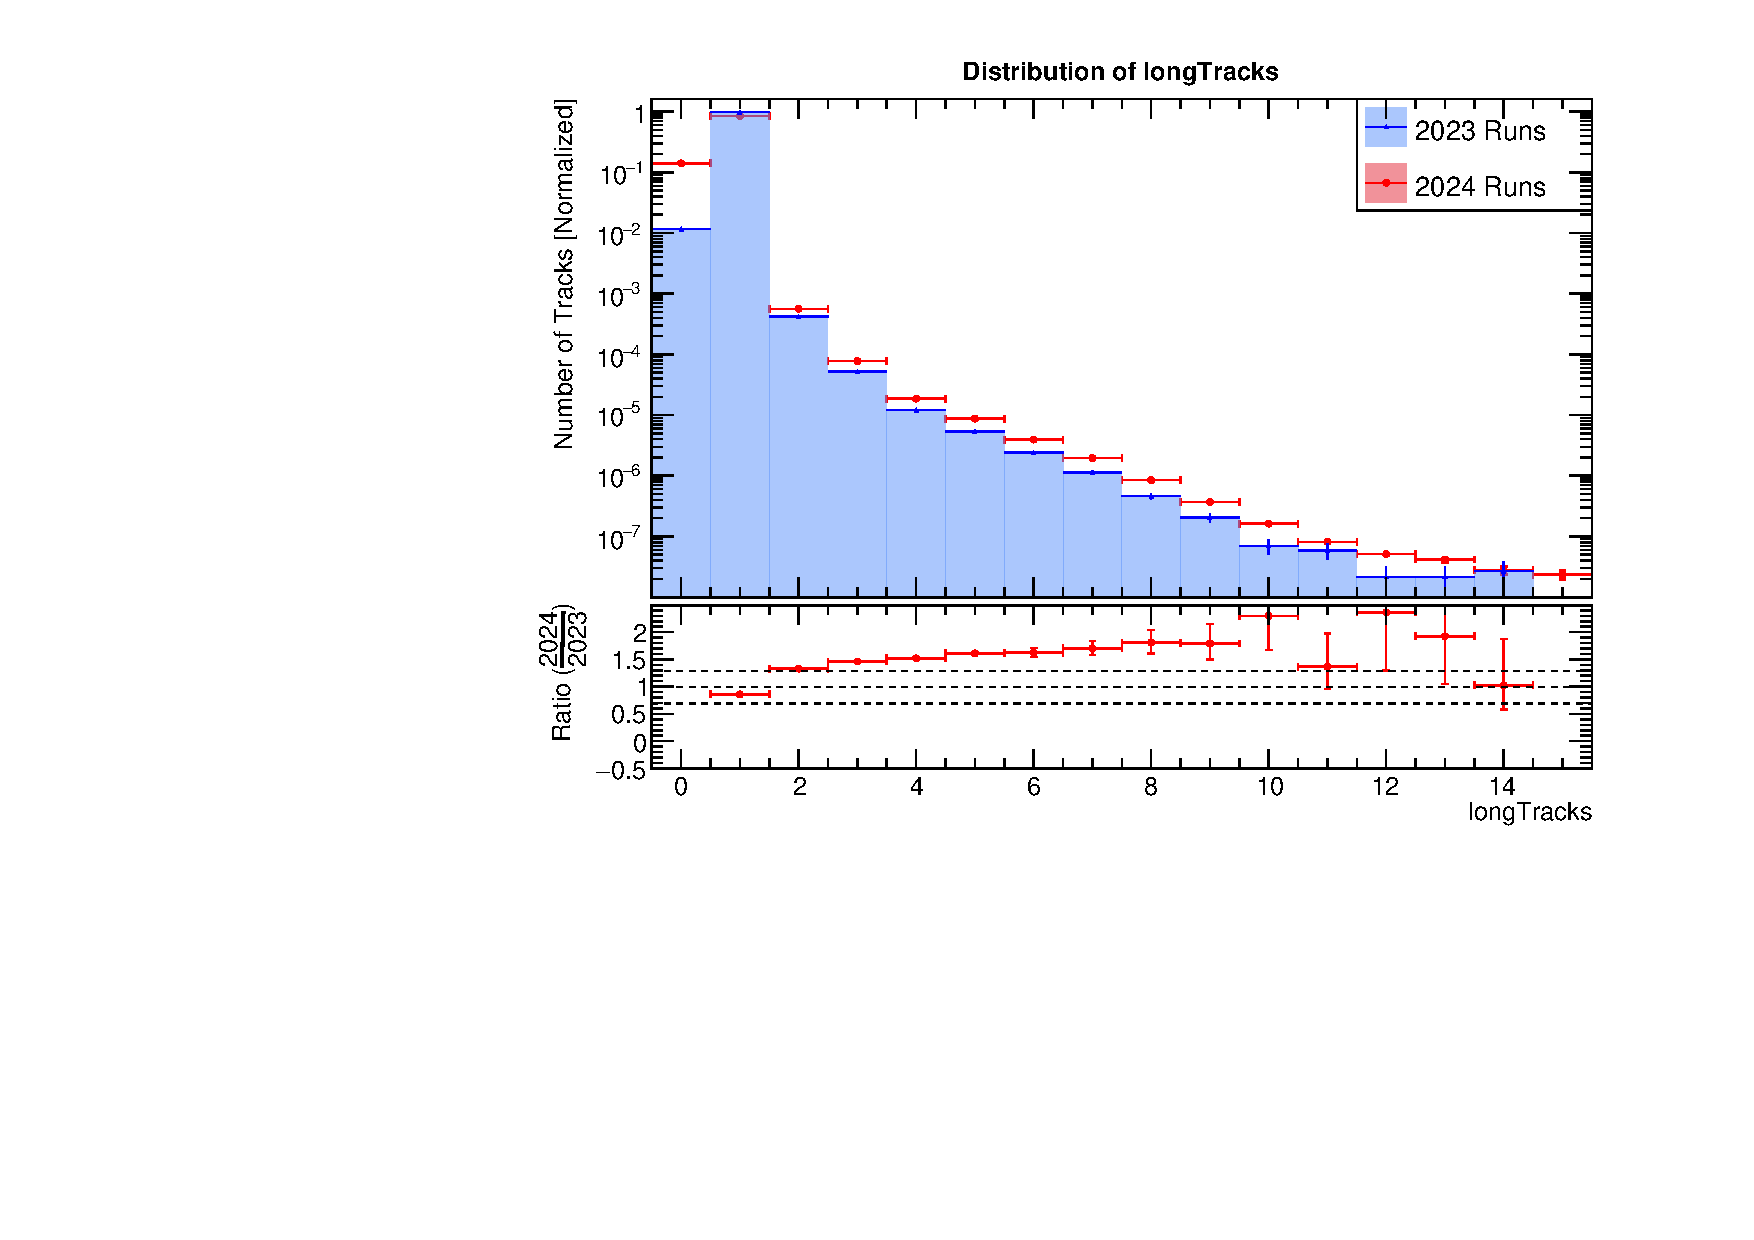
\includegraphics[width=\linewidth] {\plots/longTracks.pdf}
                \caption{Distribution of Number of Tracks}
            \end{figure}
        \end{column}
    \end{columns}
\end{frame}

\begin{frame}{Distribution of Track Charge}
    \begin{columns}
        \begin{column}{0.45\textwidth}
            \begin{itemize}
                \item We have a higher percentage of anti-muons
                \item Consistent with earlier observation of ``Much larger population of very high
                      energy positive muons''
                      \href{https://indico.cern.ch/event/1407468/contributions/5915392/attachments/2851428/4985973/2024_conversions.pdf}{[see
                                  Talk]}
            \end{itemize}
        \end{column}
        \begin{column}{0.8\textwidth}
            \begin{figure}
                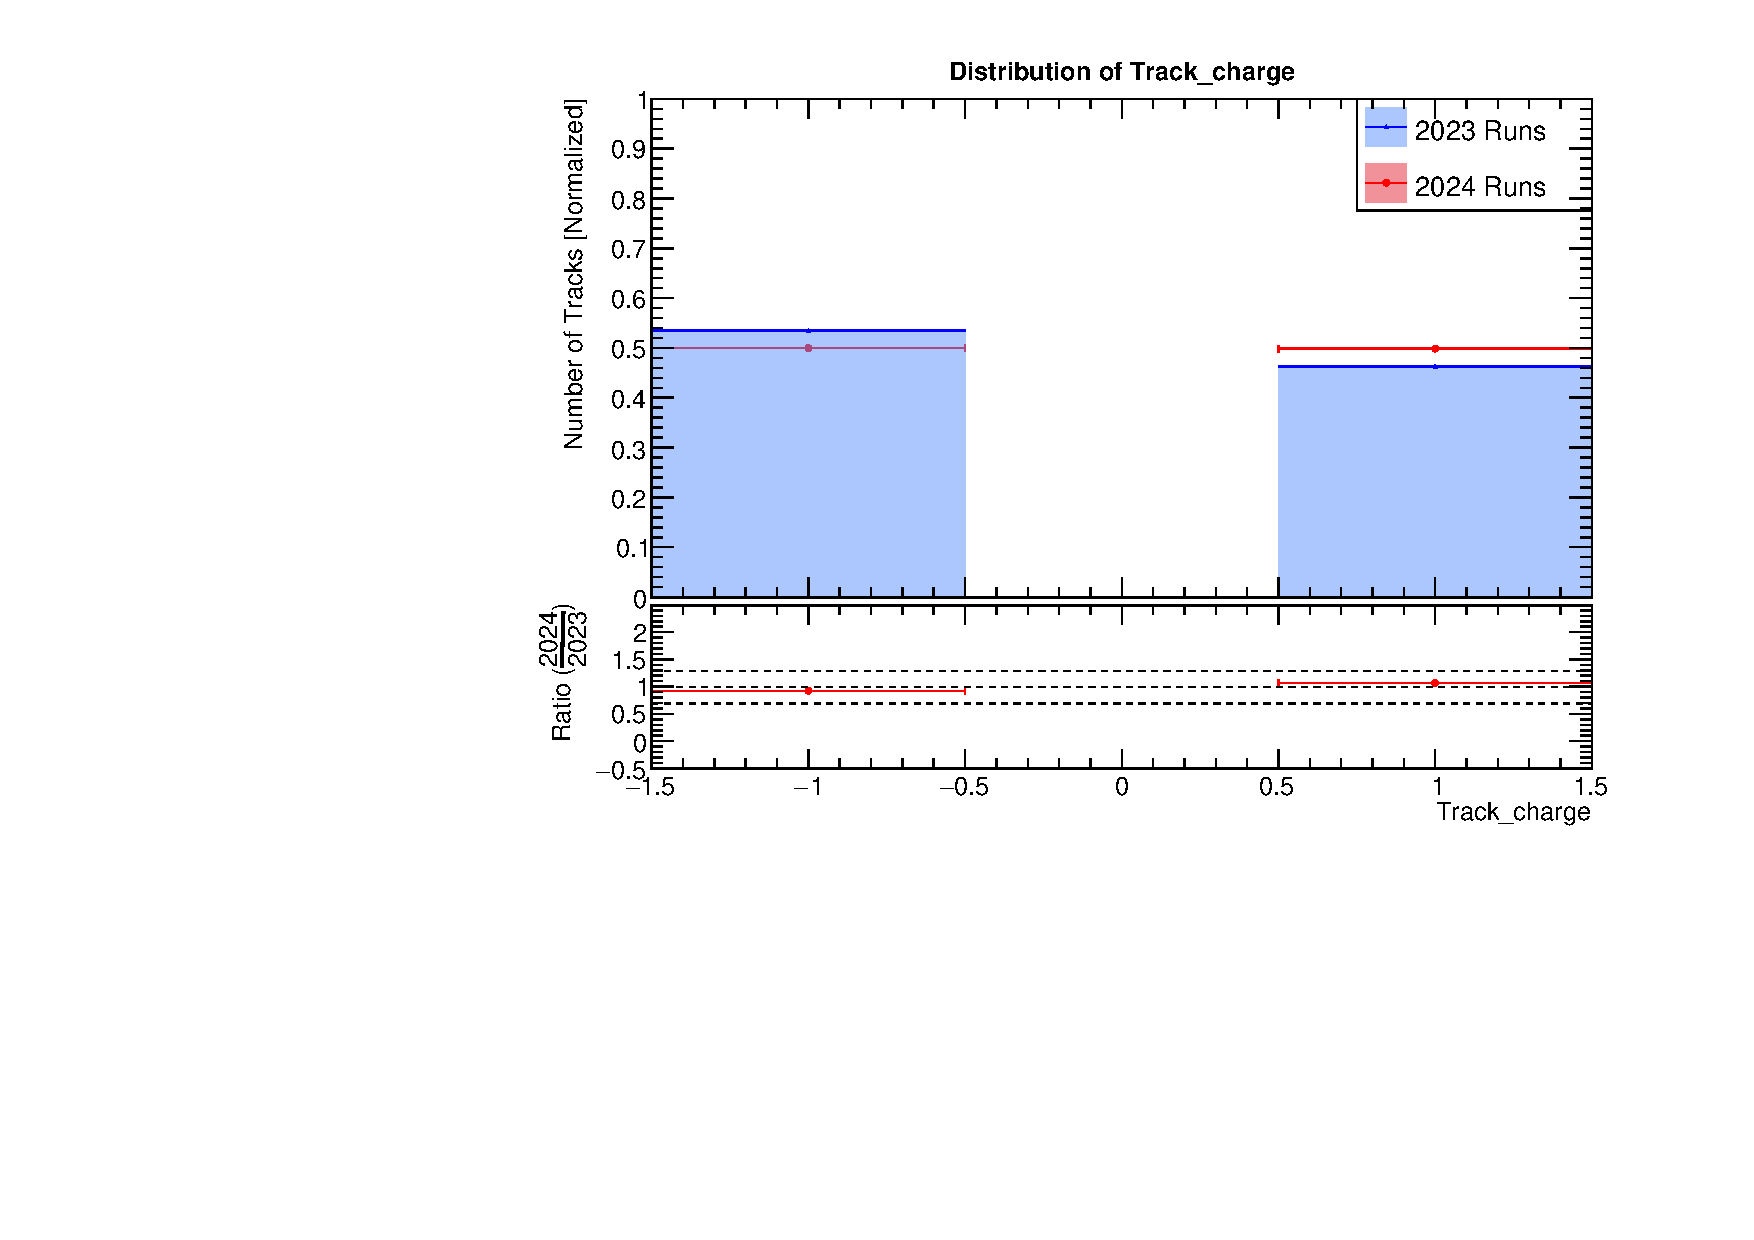
\includegraphics[width=\linewidth] {\plots/Track_charge.pdf}
                \caption{Distribution of Track Charge}
            \end{figure}
        \end{column}
    \end{columns}

\end{frame}

\begin{frame}{Distribution of Track $\chi^2$}
    \begin{columns}
        \begin{column}{0.45\textwidth}
            \begin{itemize}
                \item Overall we observe a lower Track $\chi^2$ in 2024
                \item Do we understand why?
            \end{itemize}
        \end{column}
        \begin{column}{0.8\textwidth}
            \begin{figure}
                % \begin{subfigure}
                \includegraphics[width=0.6\linewidth] {\plots/Track_chi2.pdf}
                \caption{Distribution of Track $\chi^2$}
                % \end{subfigure}
            \end{figure}
            \vspace{-0.8cm}
            \begin{figure}
                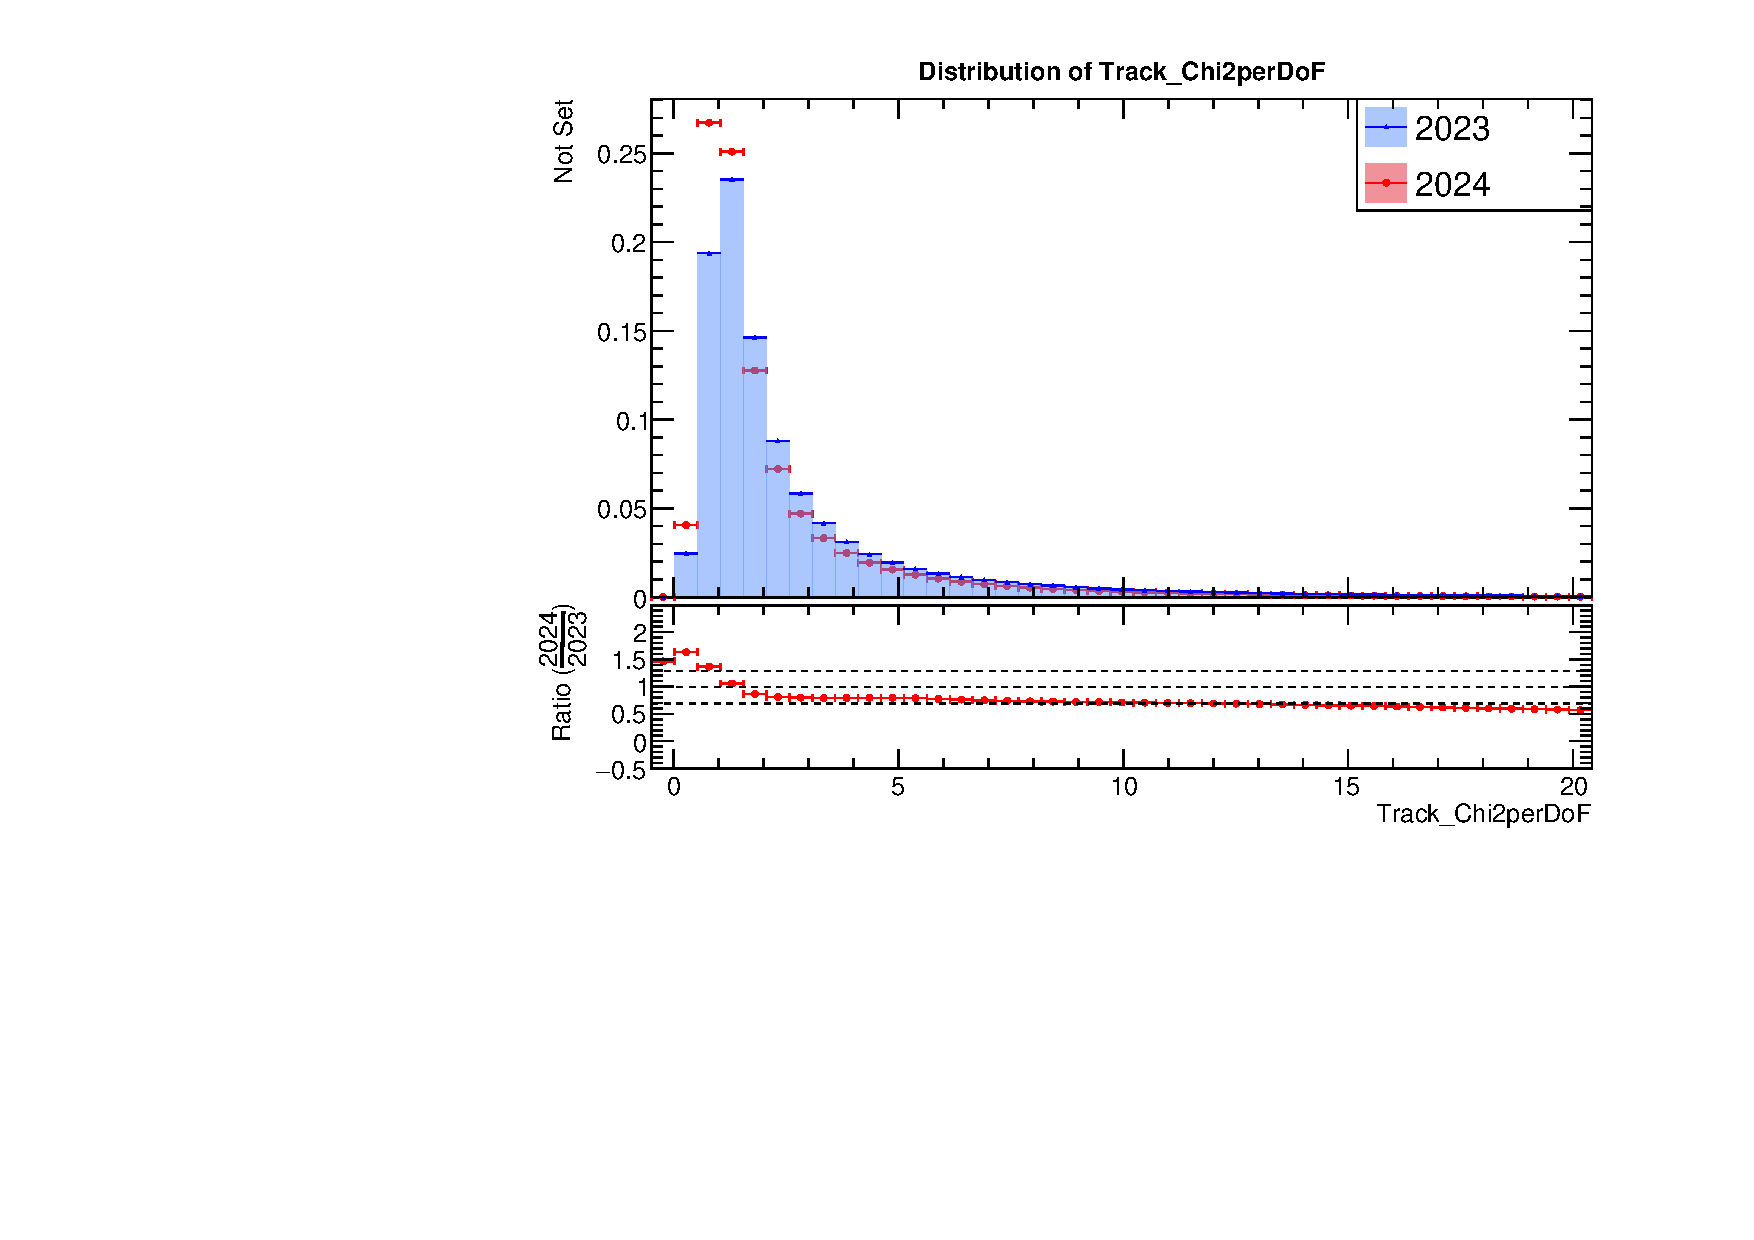
\includegraphics[width=0.6\linewidth] {\plots/Track_Chi2perDoF.pdf}
                \caption{Distribution of Track $\chi^2$ per DoF}
            \end{figure}
        \end{column}
    \end{columns}
\end{frame}

\begin{subframe}{Distribution of Track in Station}
    \begin{columns}
        \begin{column}{0.5\linewidth}
            \begin{tikzpicture}
                \draw (0,0) node[inner sep=0]{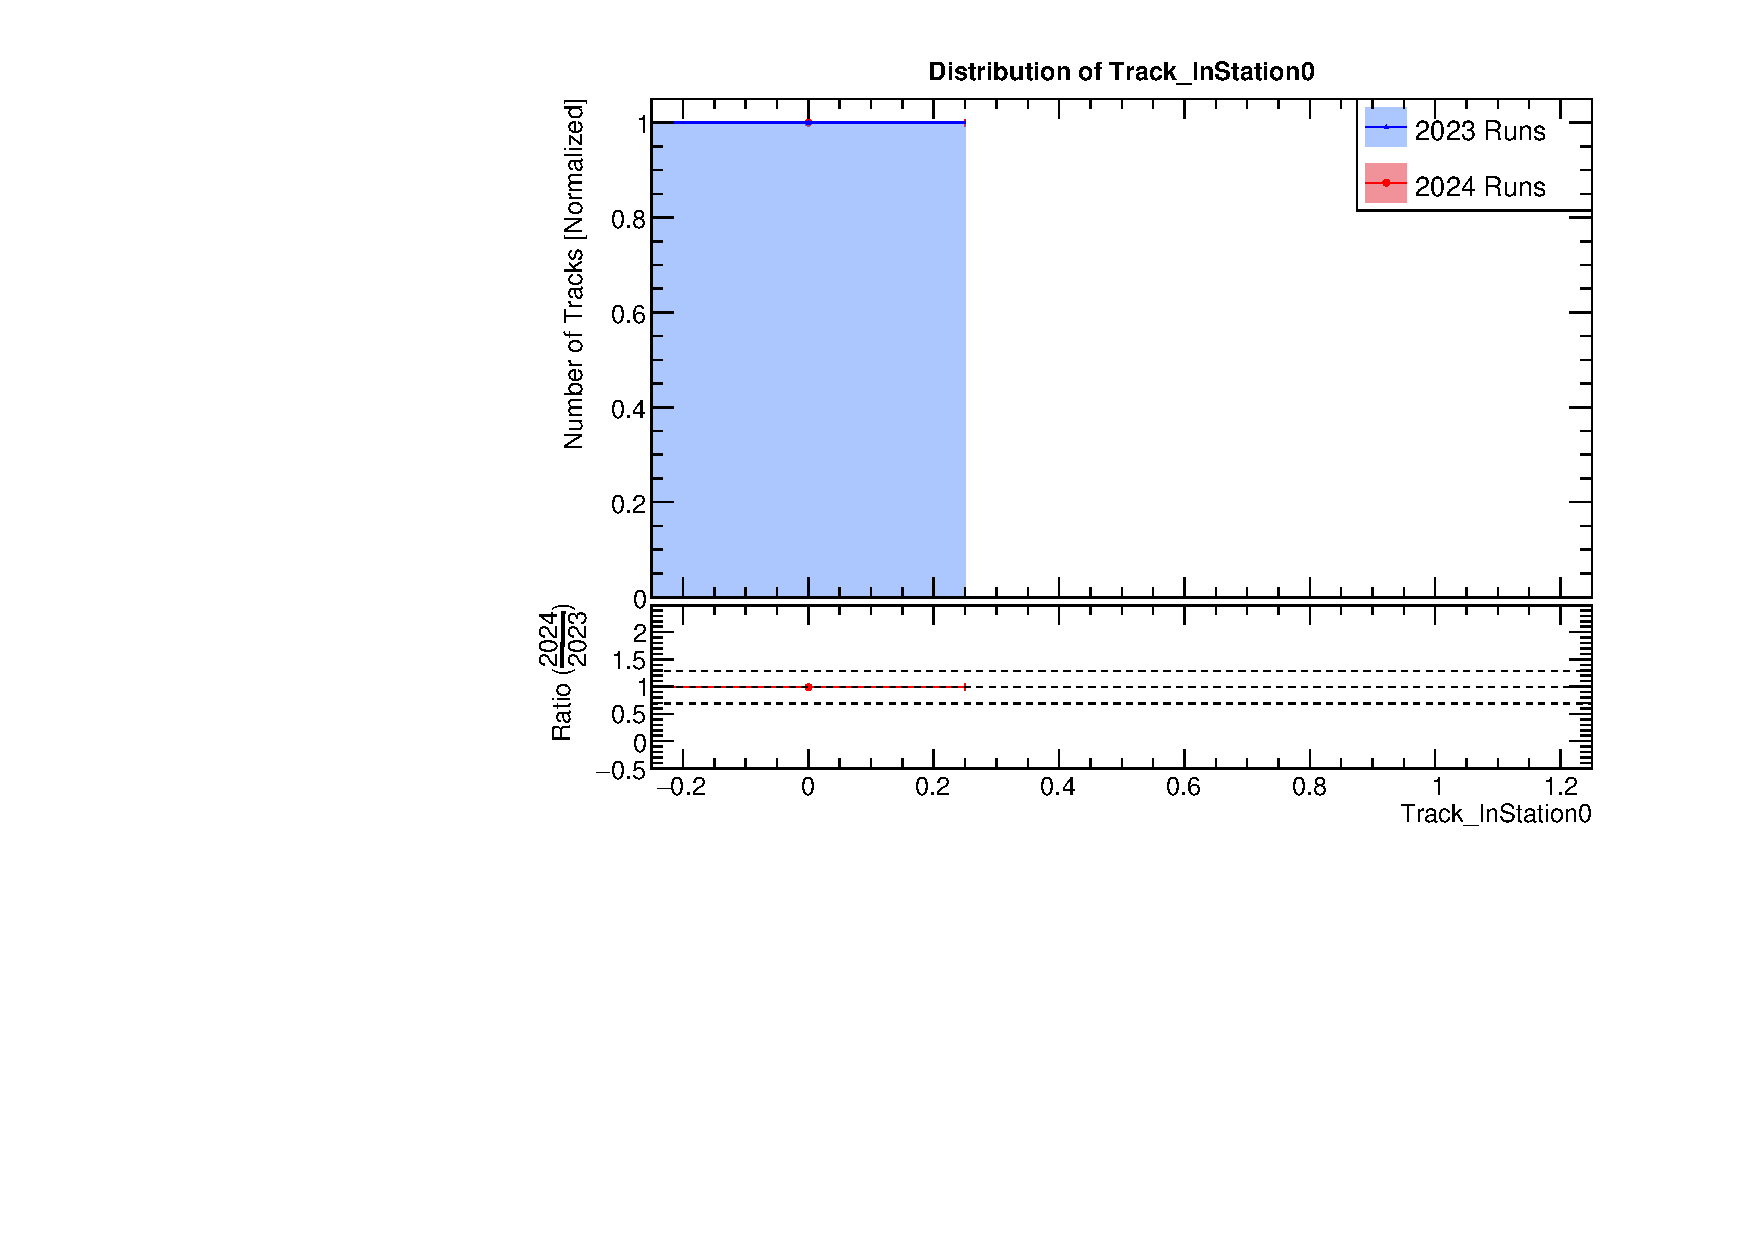
\includegraphics[width=\textwidth] {\plots/Track_InStation0.pdf}};
            \end{tikzpicture}
            \begin{tikzpicture}
                \draw (0,0) node[inner sep=0]{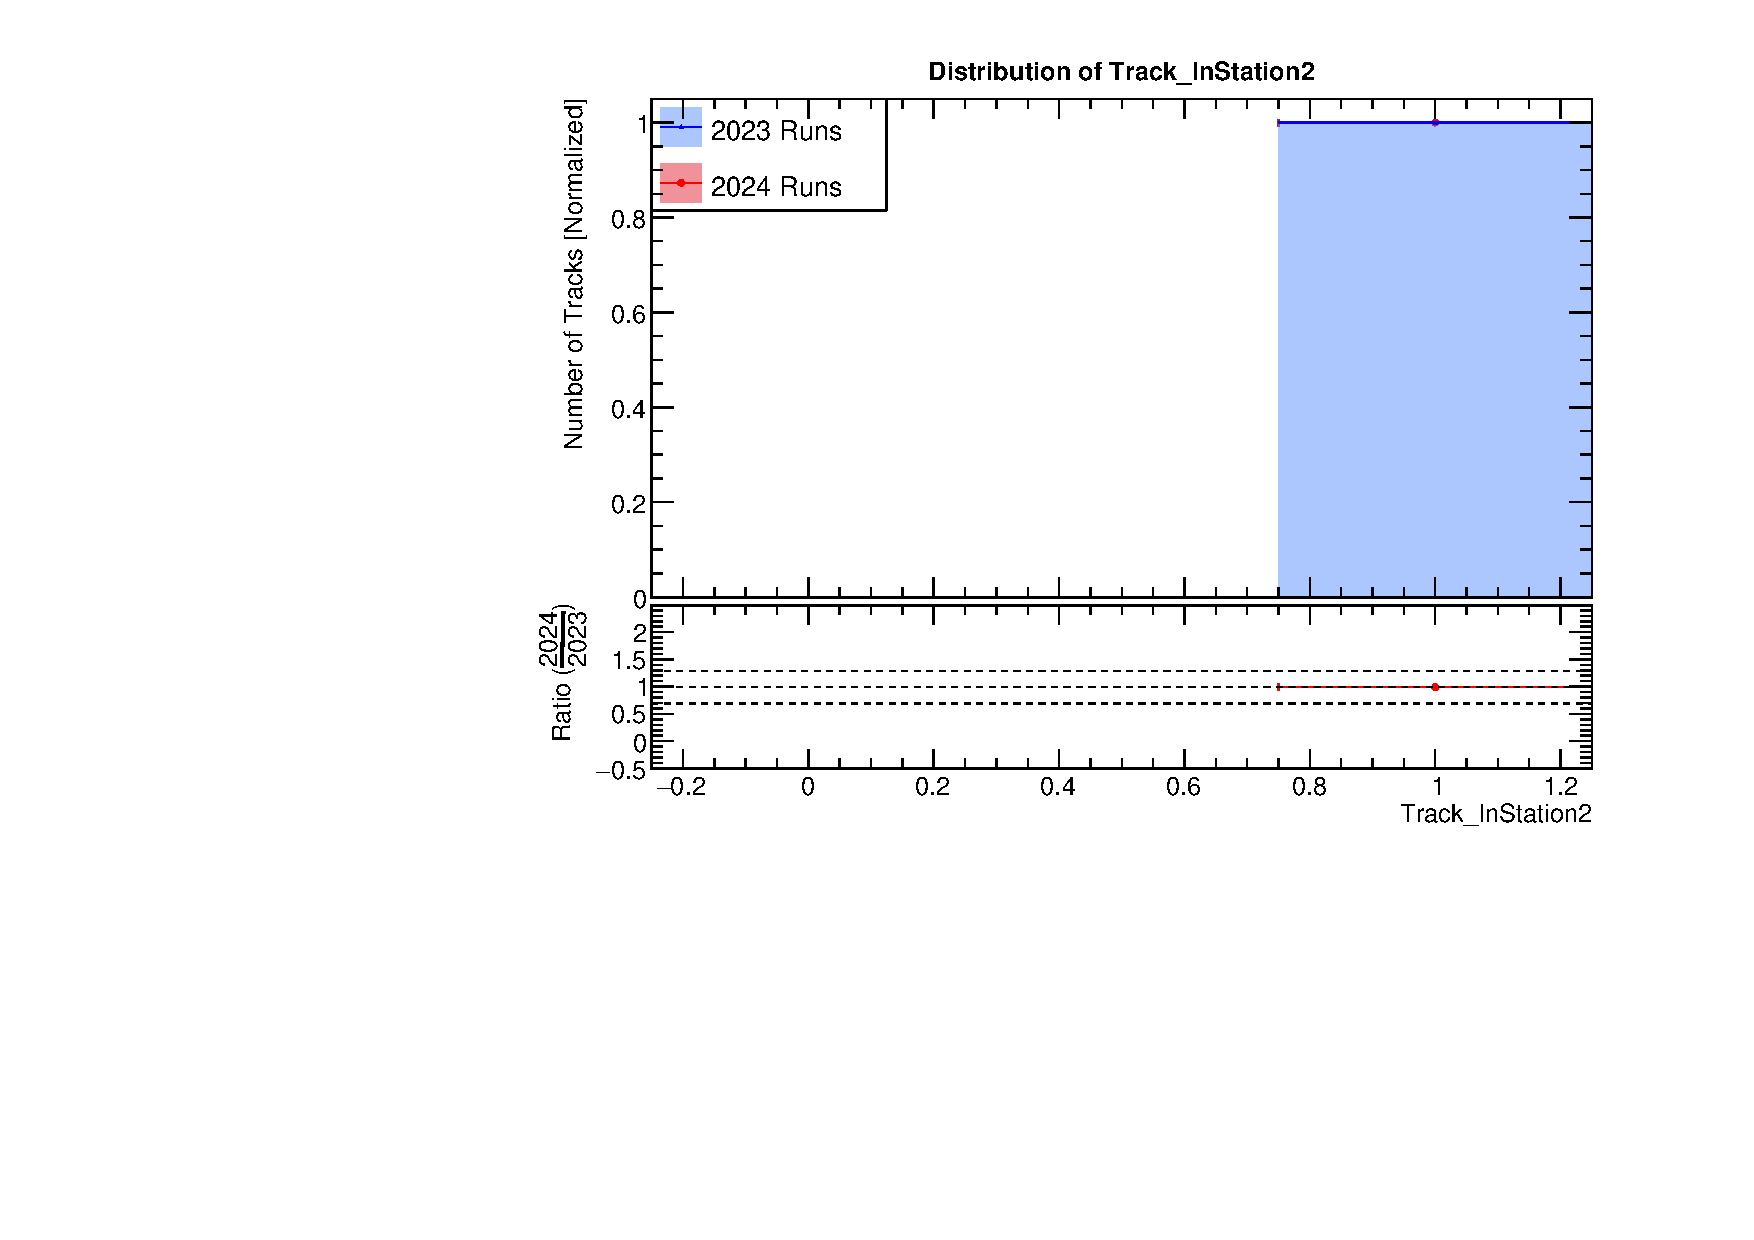
\includegraphics[width=\textwidth] {\plots/Track_InStation2.pdf}};
            \end{tikzpicture}
        \end{column}
        \begin{column}{0.5\linewidth}
            \begin{tikzpicture}
                \draw (0,0) node[inner sep=0]{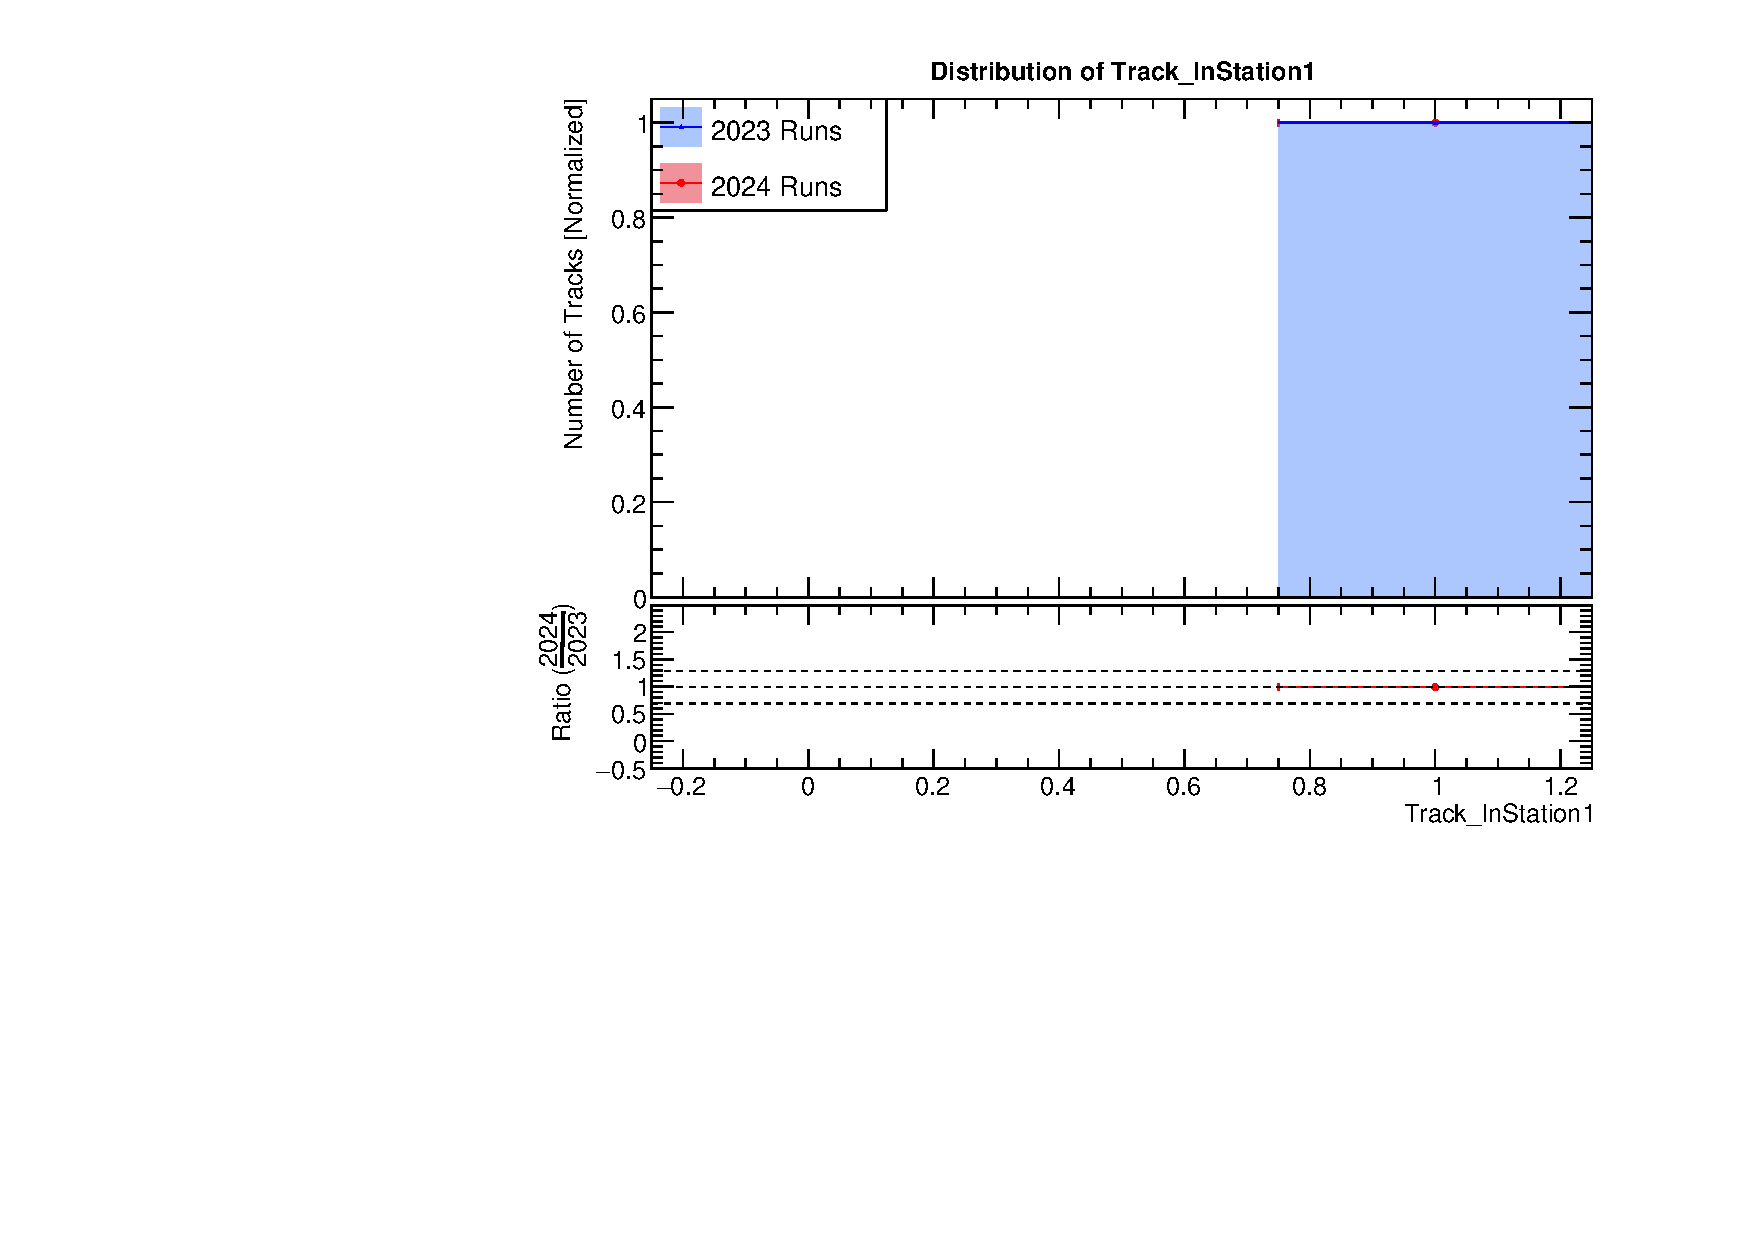
\includegraphics[width=\textwidth] {\plots/Track_InStation1.pdf}};
            \end{tikzpicture}
            \begin{tikzpicture}
                \draw (0,0) node[inner sep=0]{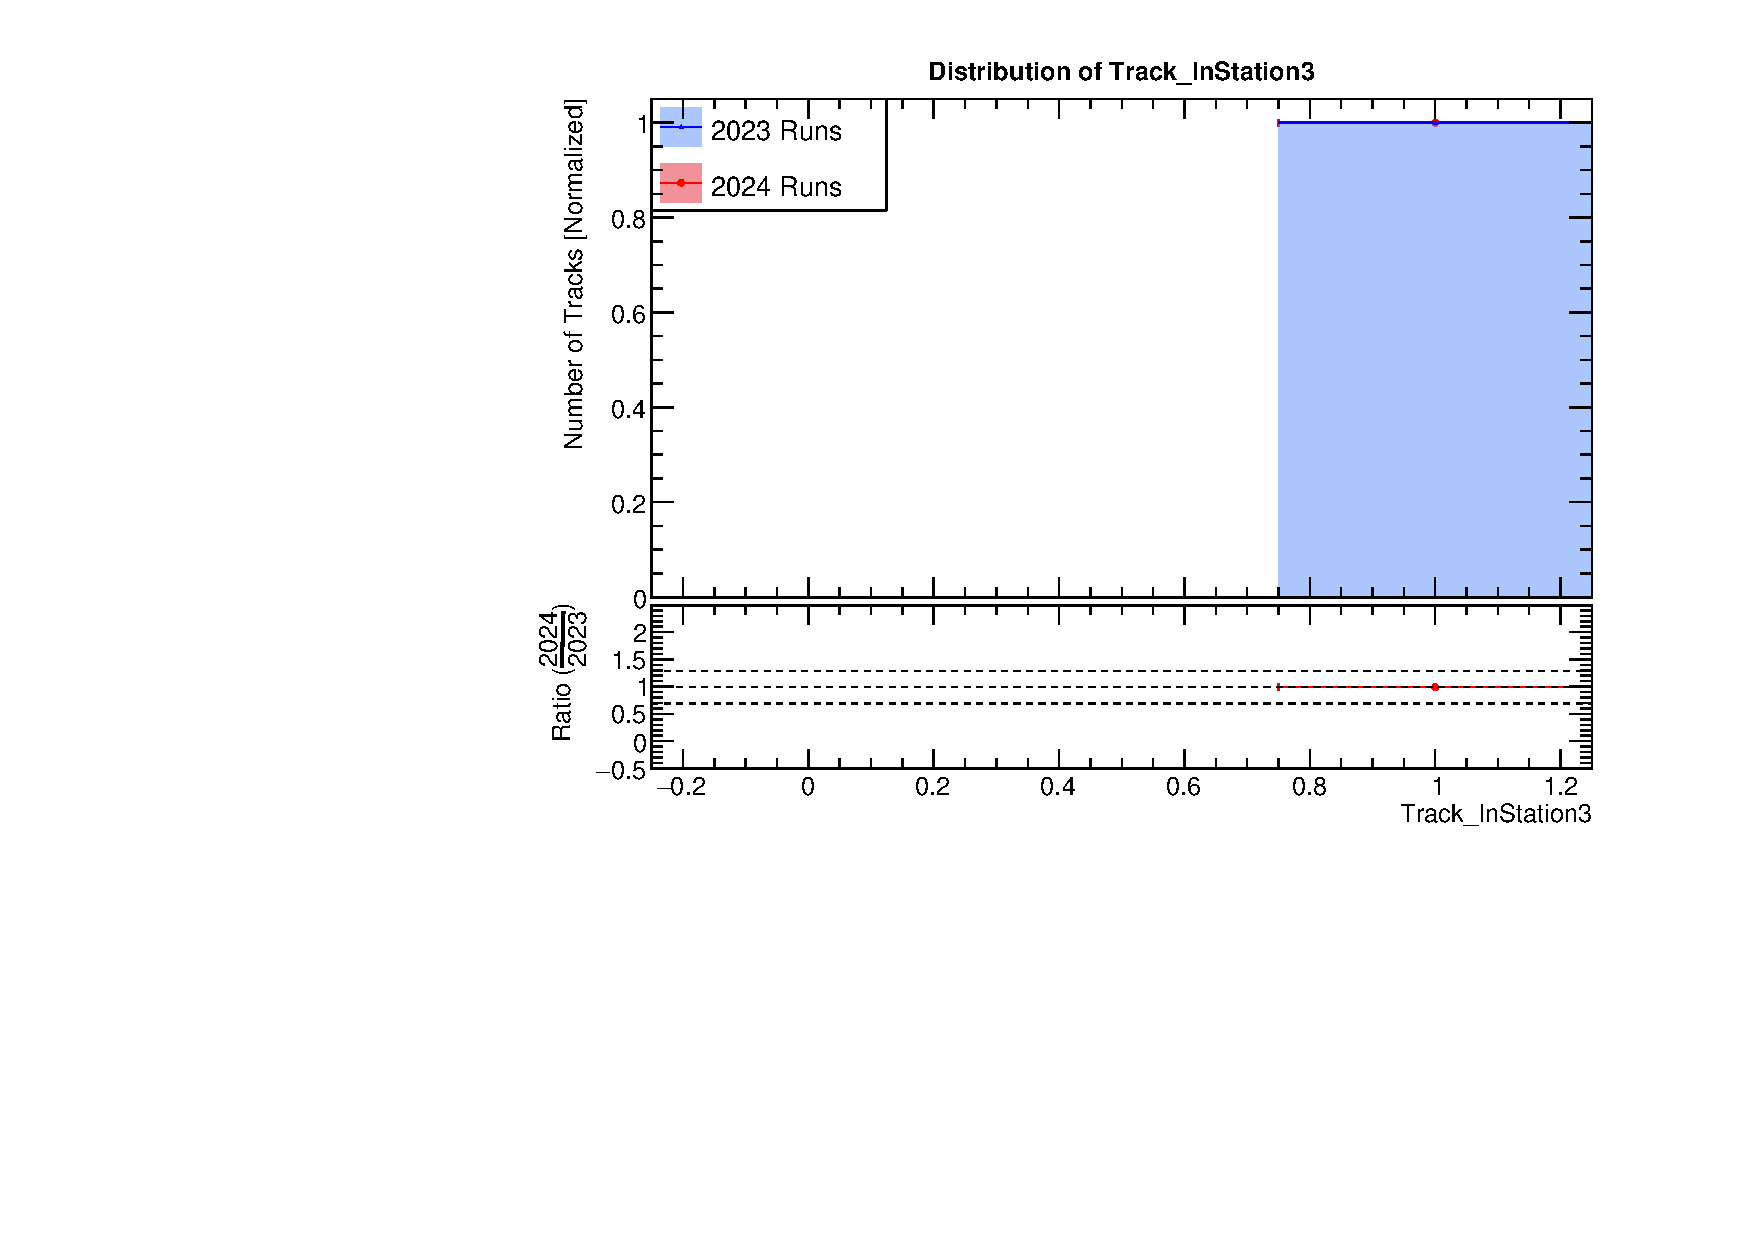
\includegraphics[width=\textwidth] {\plots/Track_InStation3.pdf}};
            \end{tikzpicture}
        \end{column}
    \end{columns}
    \scriptsize{There are always 0 tracks in Station0. Possibly an issue in NTupleDumper. Haven't located this yet.}
\end{subframe}

\begin{subframe}{Track\_nLayers}
    \begin{figure}
        \begin{tikzpicture}
            \draw (0,0) node[inner sep=0]{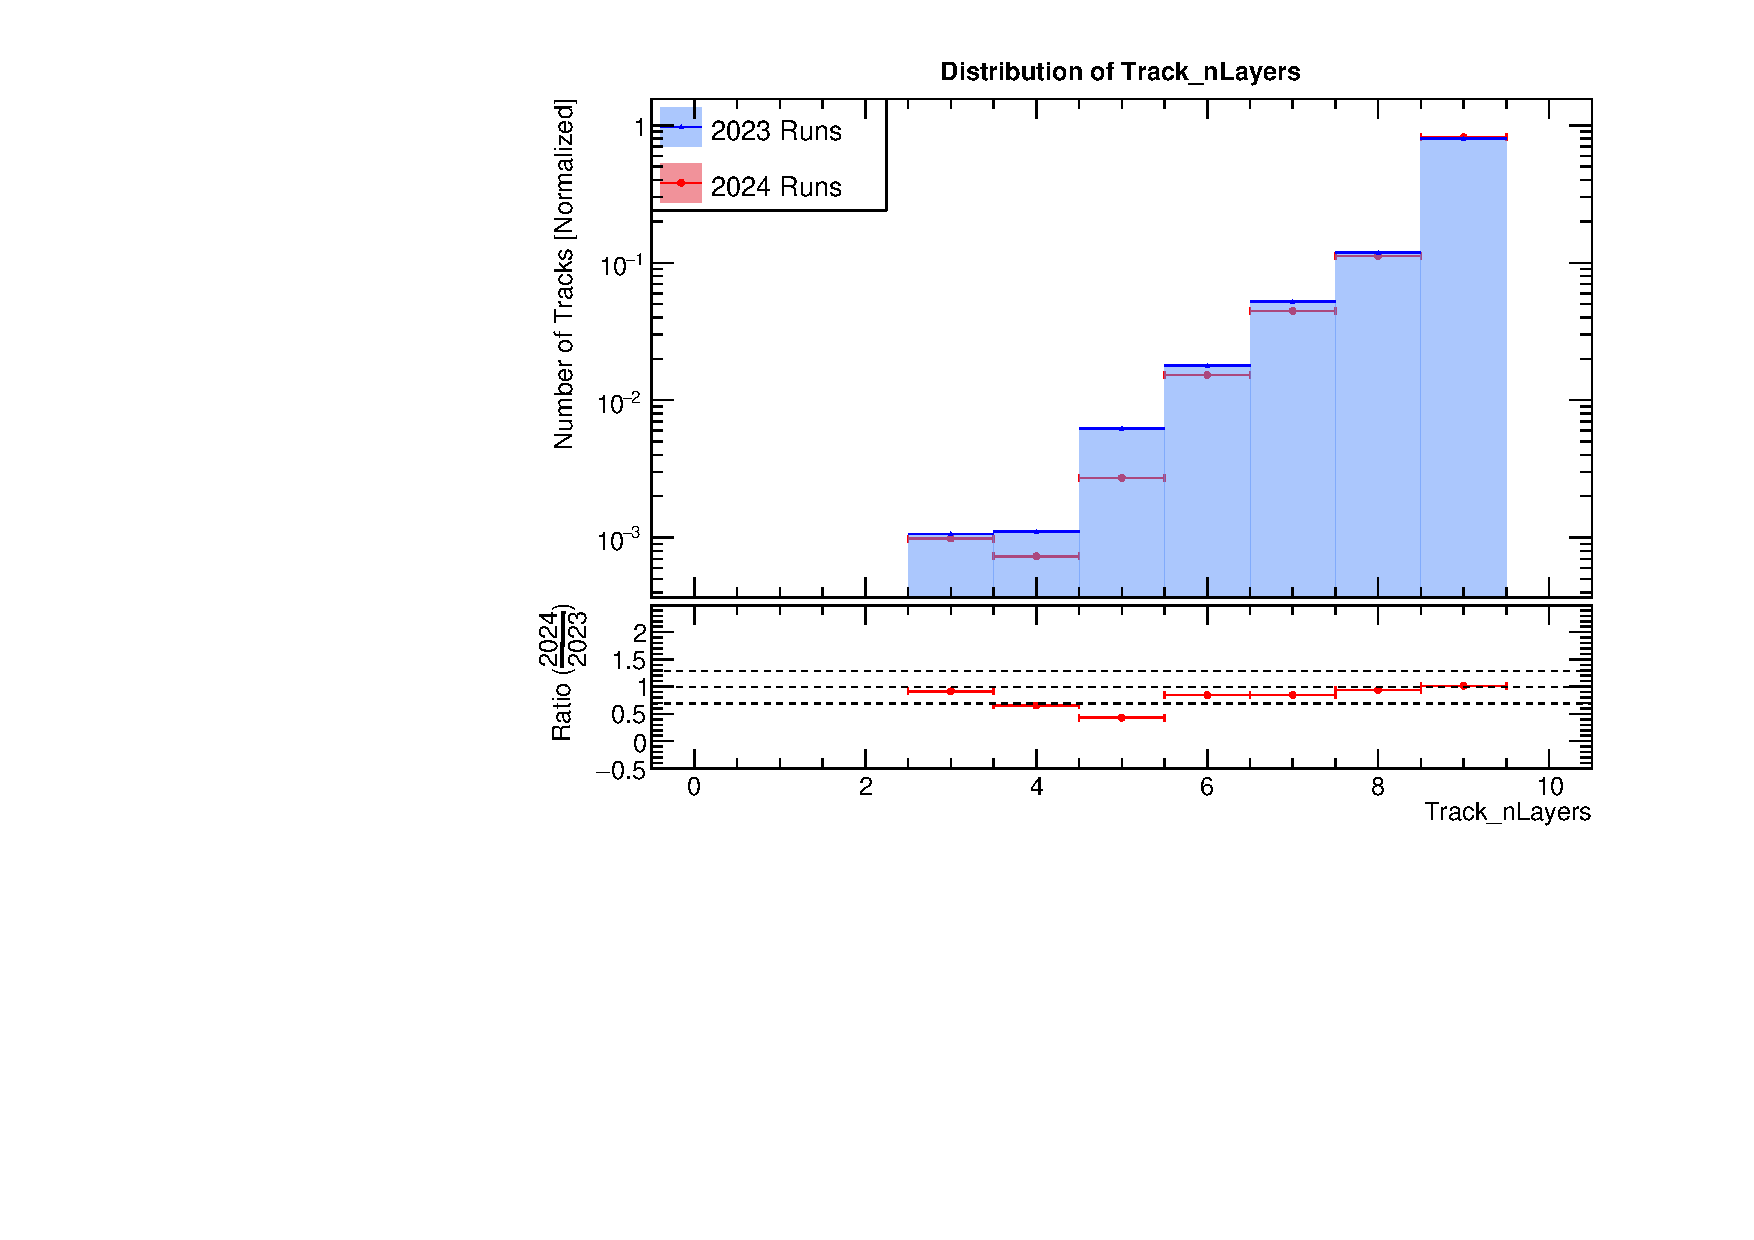
\includegraphics[width=\textwidth] {\plots/Track_nLayers.pdf}};
        \end{tikzpicture}
        \caption{Distribution of Track\_nLayers}
    \end{figure}
\end{subframe}

\begin{frame}{Track Propagation Error}
    \begin{columns}
        \begin{column}{0.3 \linewidth}
            \begin{itemize}
                \item Much higher Track Propagation Error in 2024 !
                \item How does this affect the track reconstruction?
            \end{itemize}
        \end{column}
    \begin{column}{0.8 \linewidth}
        \begin{figure}
            \begin{tikzpicture}
                \draw (0,0) node[inner sep=0]{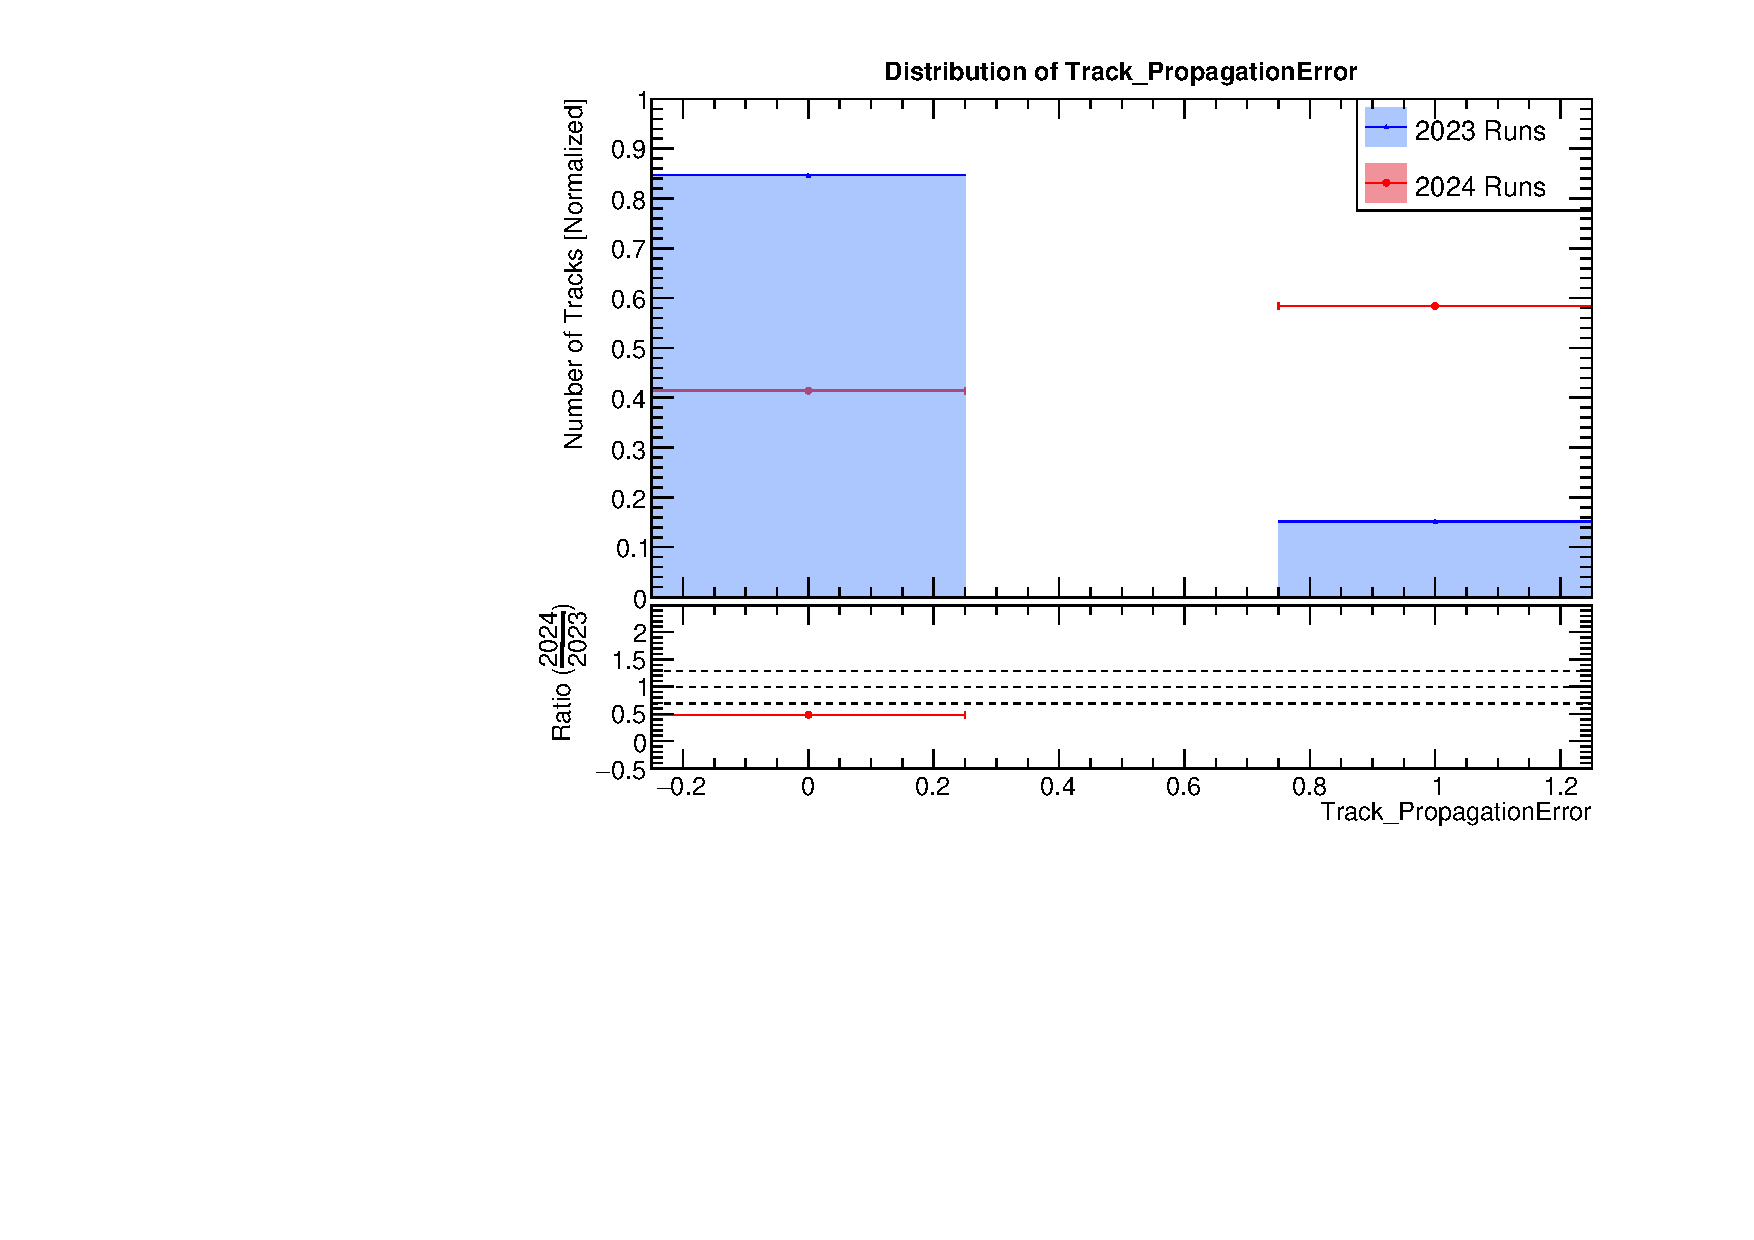
\includegraphics[width=\textwidth] {\plots/Track_PropagationError.pdf}};
            \end{tikzpicture}
            \caption{Distribution of Track Propagation Error}
        \end{figure}
    \end{column}
    \end{columns}
\end{frame}
\begin{frame}{Track Positions (x, y)}
    \centering
    % \underline{Basic Plot Parameters}
    \begin{itemize}
        \item Vetonu
        \item VetoStation 1 [in Backup]
        \item VetoStation 2 [in Backup]
        \item Trigger/Timing Station [in Backup]
        \item Tracking Station 1
        \item Tracking Station 3
        \item Preshower 1 [in Backup]
        \item Preshower 2 [in Backup]
        \item Calo
        \item Max Radius
    \end{itemize}
\end{frame}

\begin{frame}{Track Positions at Vetonu}
    \begin{columns}
        \begin{column}{0.5\textwidth}
            \begin{figure}
                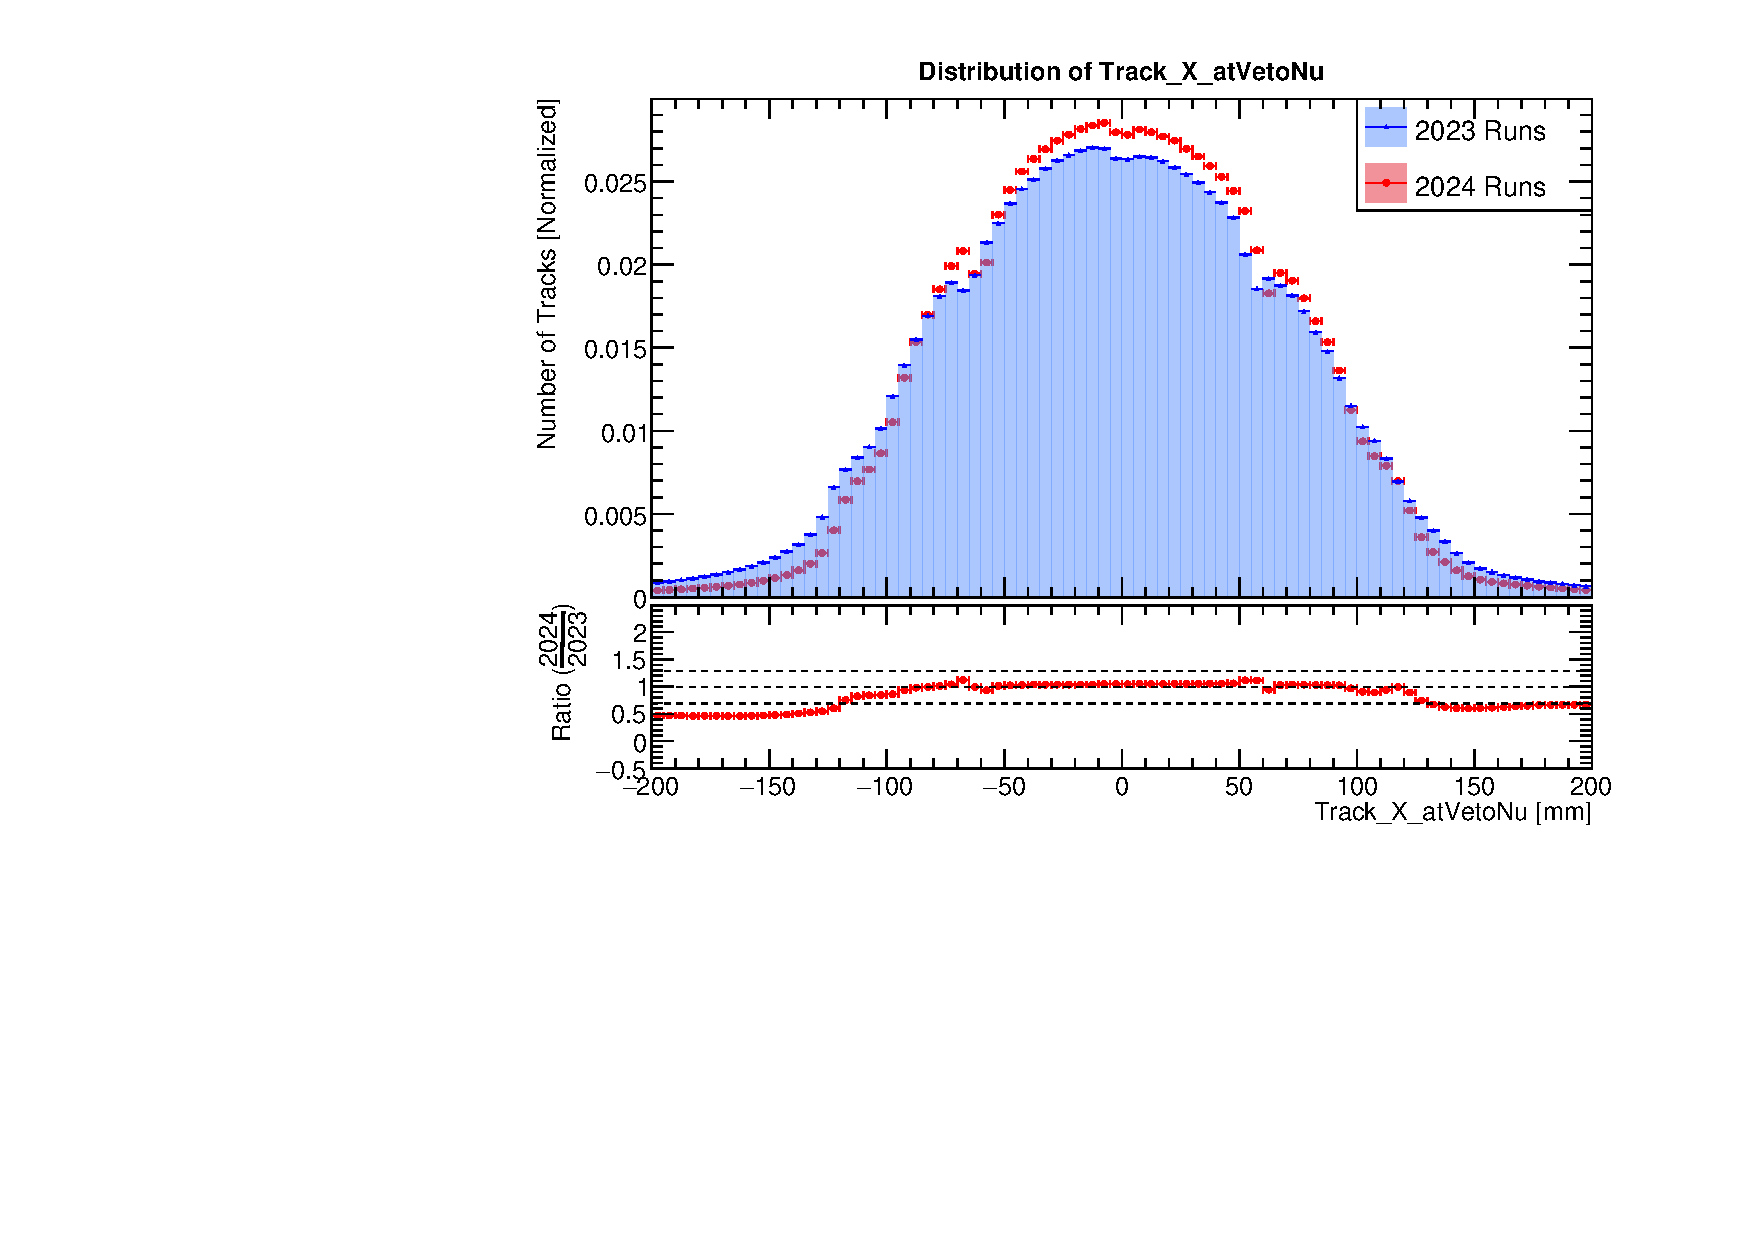
\includegraphics[width=\linewidth] {\plots/Track_X_atVetoNu.pdf}
                \caption{Track Position x at VetoNu}
            \end{figure}
        \end{column}
        \begin{column}{0.5\textwidth}
            \begin{figure}
                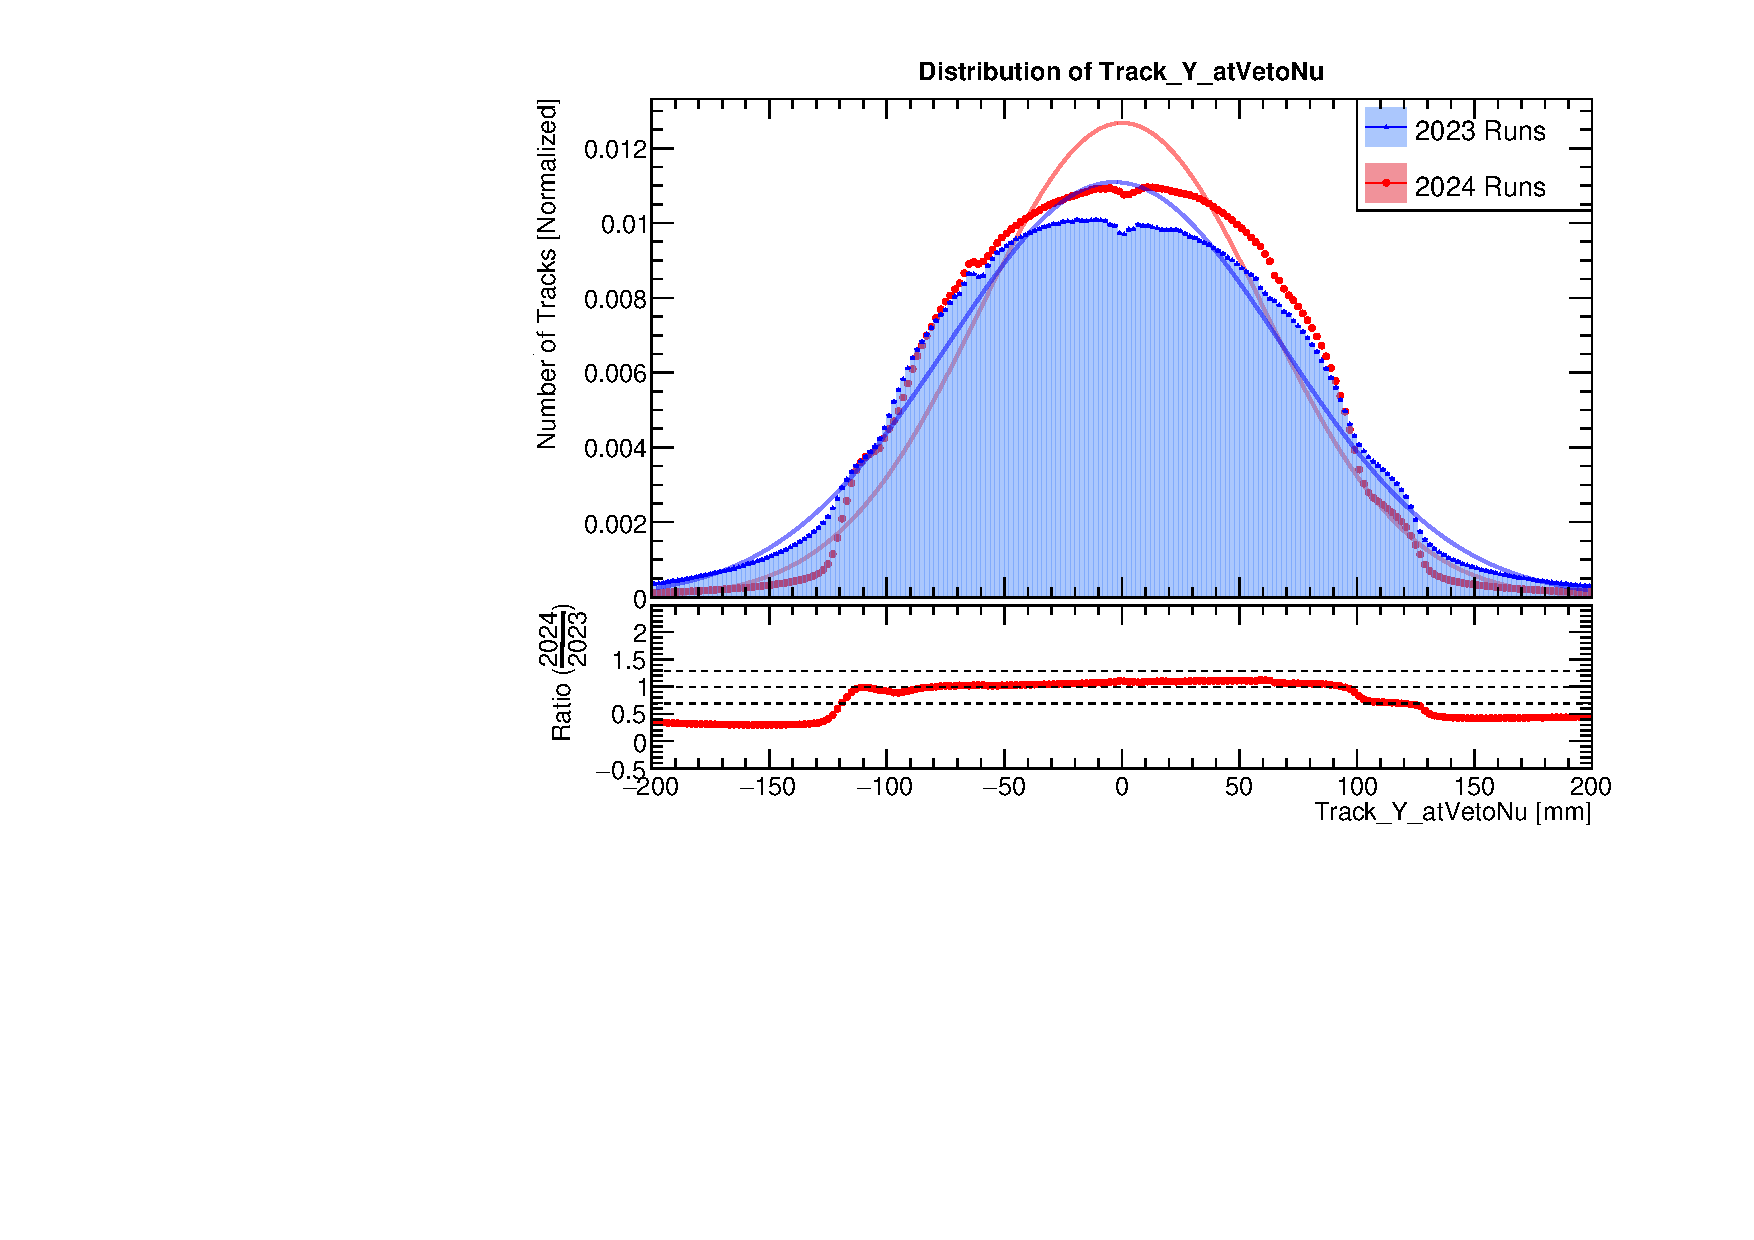
\includegraphics[width=\linewidth] {\plots/Track_Y_atVetoNu.pdf}
                \caption{Track Position y at VetoNu}
            \end{figure}
        \end{column}
    \end{columns}
    \begin{itemize}
        \item Sharper Distribution in 2024: More particles on center? REF?
              % \item The ypeak has shifted from -12.5 mm to 12.5 mm.
        \item The ypeak has shifted to the positive side. Expected with the change in beam crossing angle
        % \item Beam crossing angle went 160 $\mu$Rad downward to 160 $\mu$Rad upwards. Thus we
            %   expect the peak y positions to go from negative to positive
        % \item Offset went from [6.5 cm CHECK THIS?] Calculations show 1.18 cm.
        \item Same comments hold for the rest of the positions.
    \end{itemize}
\end{frame}

\begin{subframe}{Track Positions at Veto Station 1 [SKIP]}
    \begin{columns}
        \begin{column}{0.5\textwidth}
            \begin{figure}
                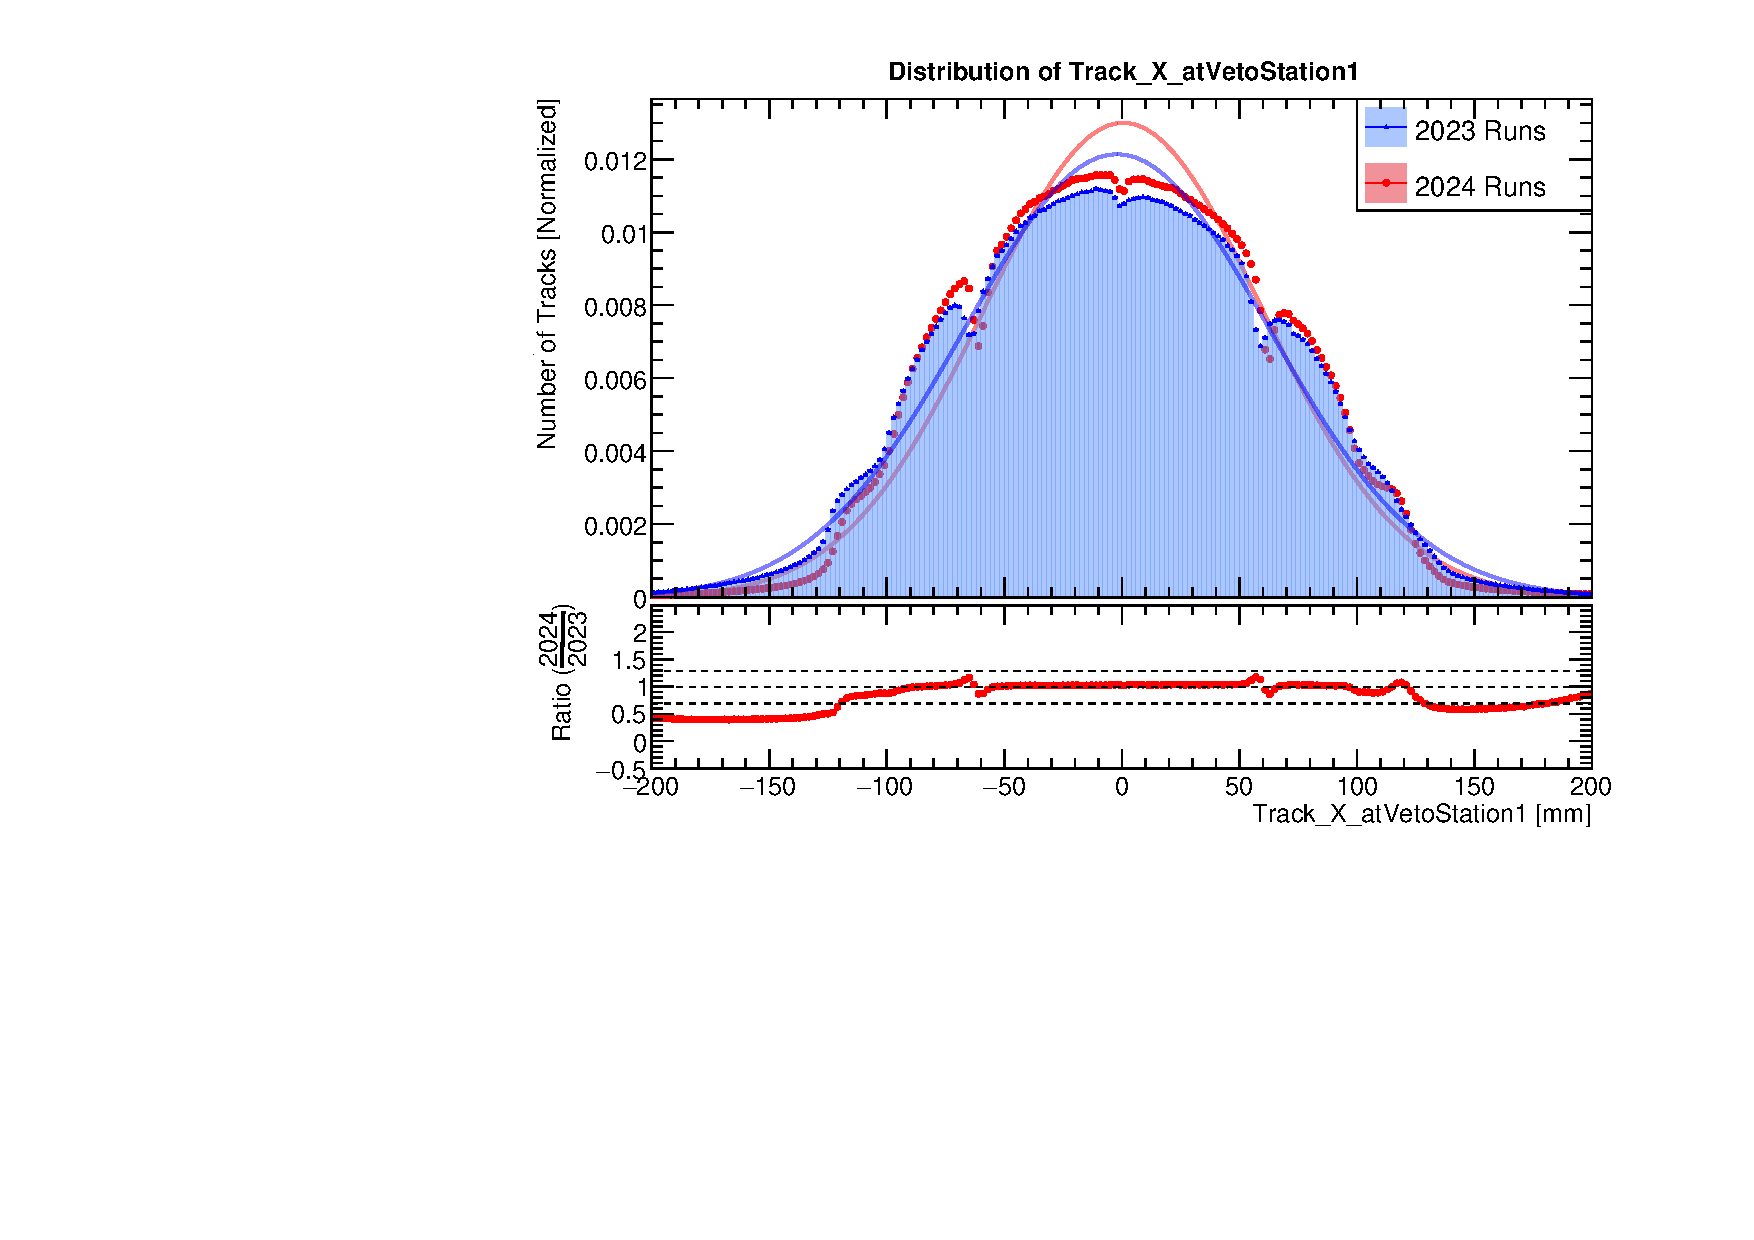
\includegraphics[width=\linewidth] {\plots/Track_X_atVetoStation1.pdf}
                \caption{Track Position x at Veto Station 1}
            \end{figure}
        \end{column}
        \begin{column}{0.5\textwidth}
            \begin{figure}
                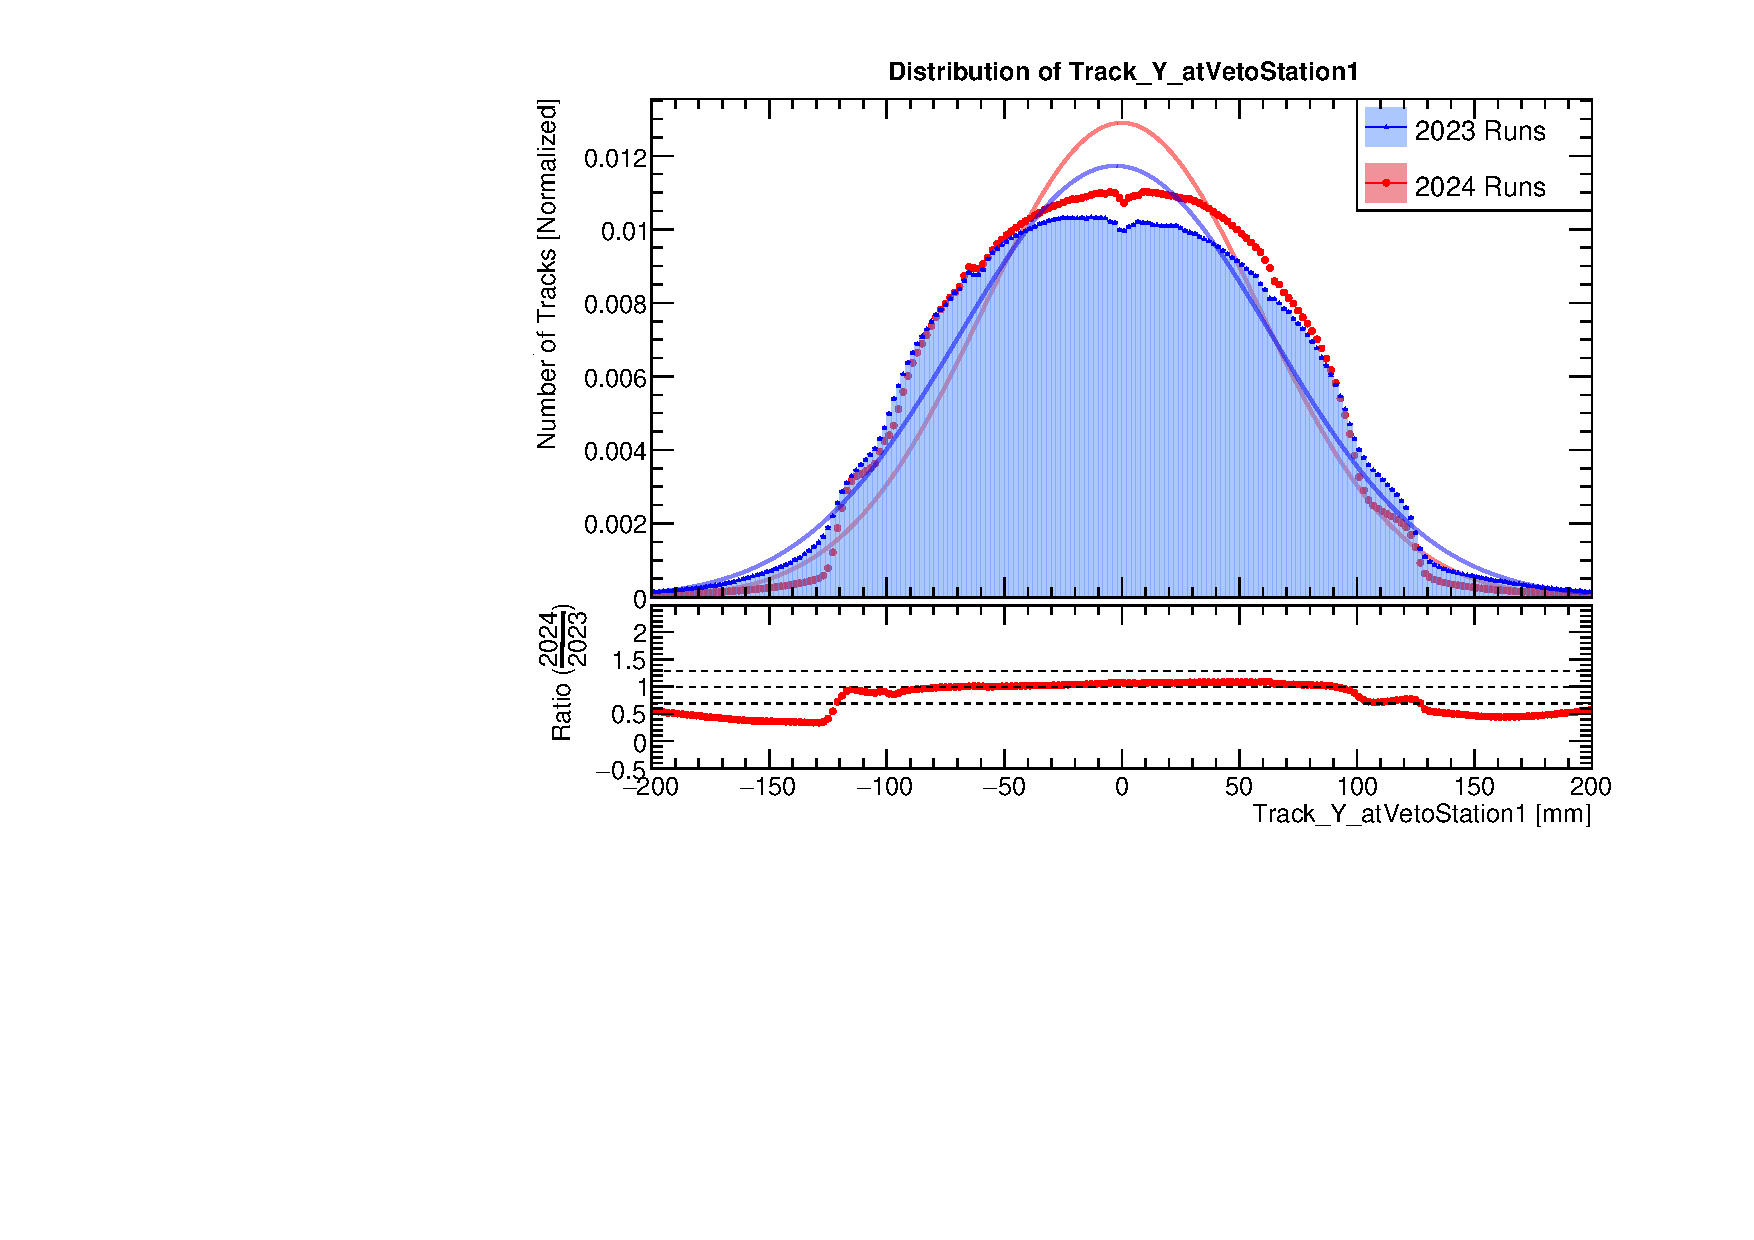
\includegraphics[width=\linewidth] {\plots/Track_Y_atVetoStation1.pdf}
                \caption{Track Position y at Veto Station 1}
            \end{figure}
        \end{column}
    \end{columns}
\end{subframe}

\begin{subframe}{Track Positions at Veto Station 2 [SKIP]}
    \begin{columns}
        \begin{column}{0.5\textwidth}
            \begin{figure}
                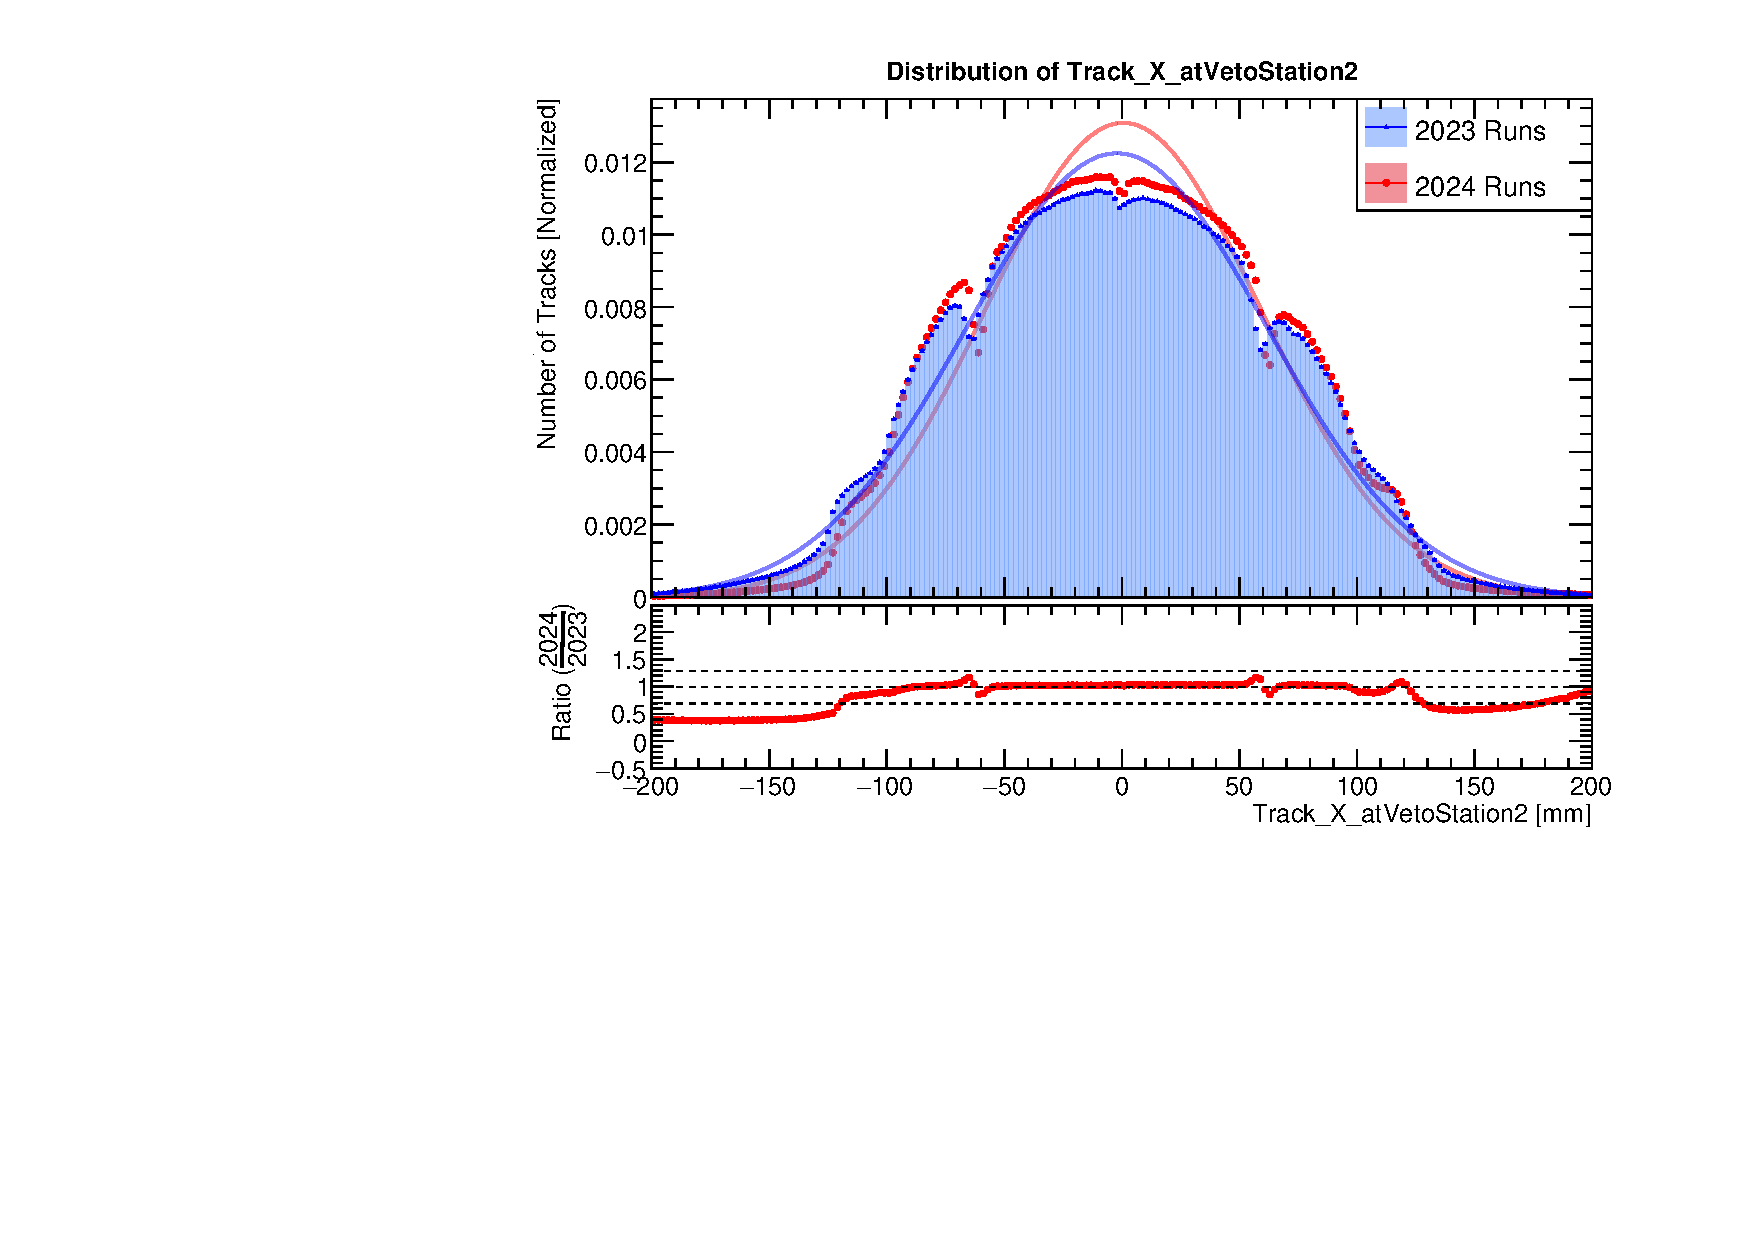
\includegraphics[width=\linewidth] {\plots/Track_X_atVetoStation2.pdf}
                \caption{Track Position x at Veto Station 2}
            \end{figure}
        \end{column}
        \begin{column}{0.5\textwidth}
            \begin{figure}
                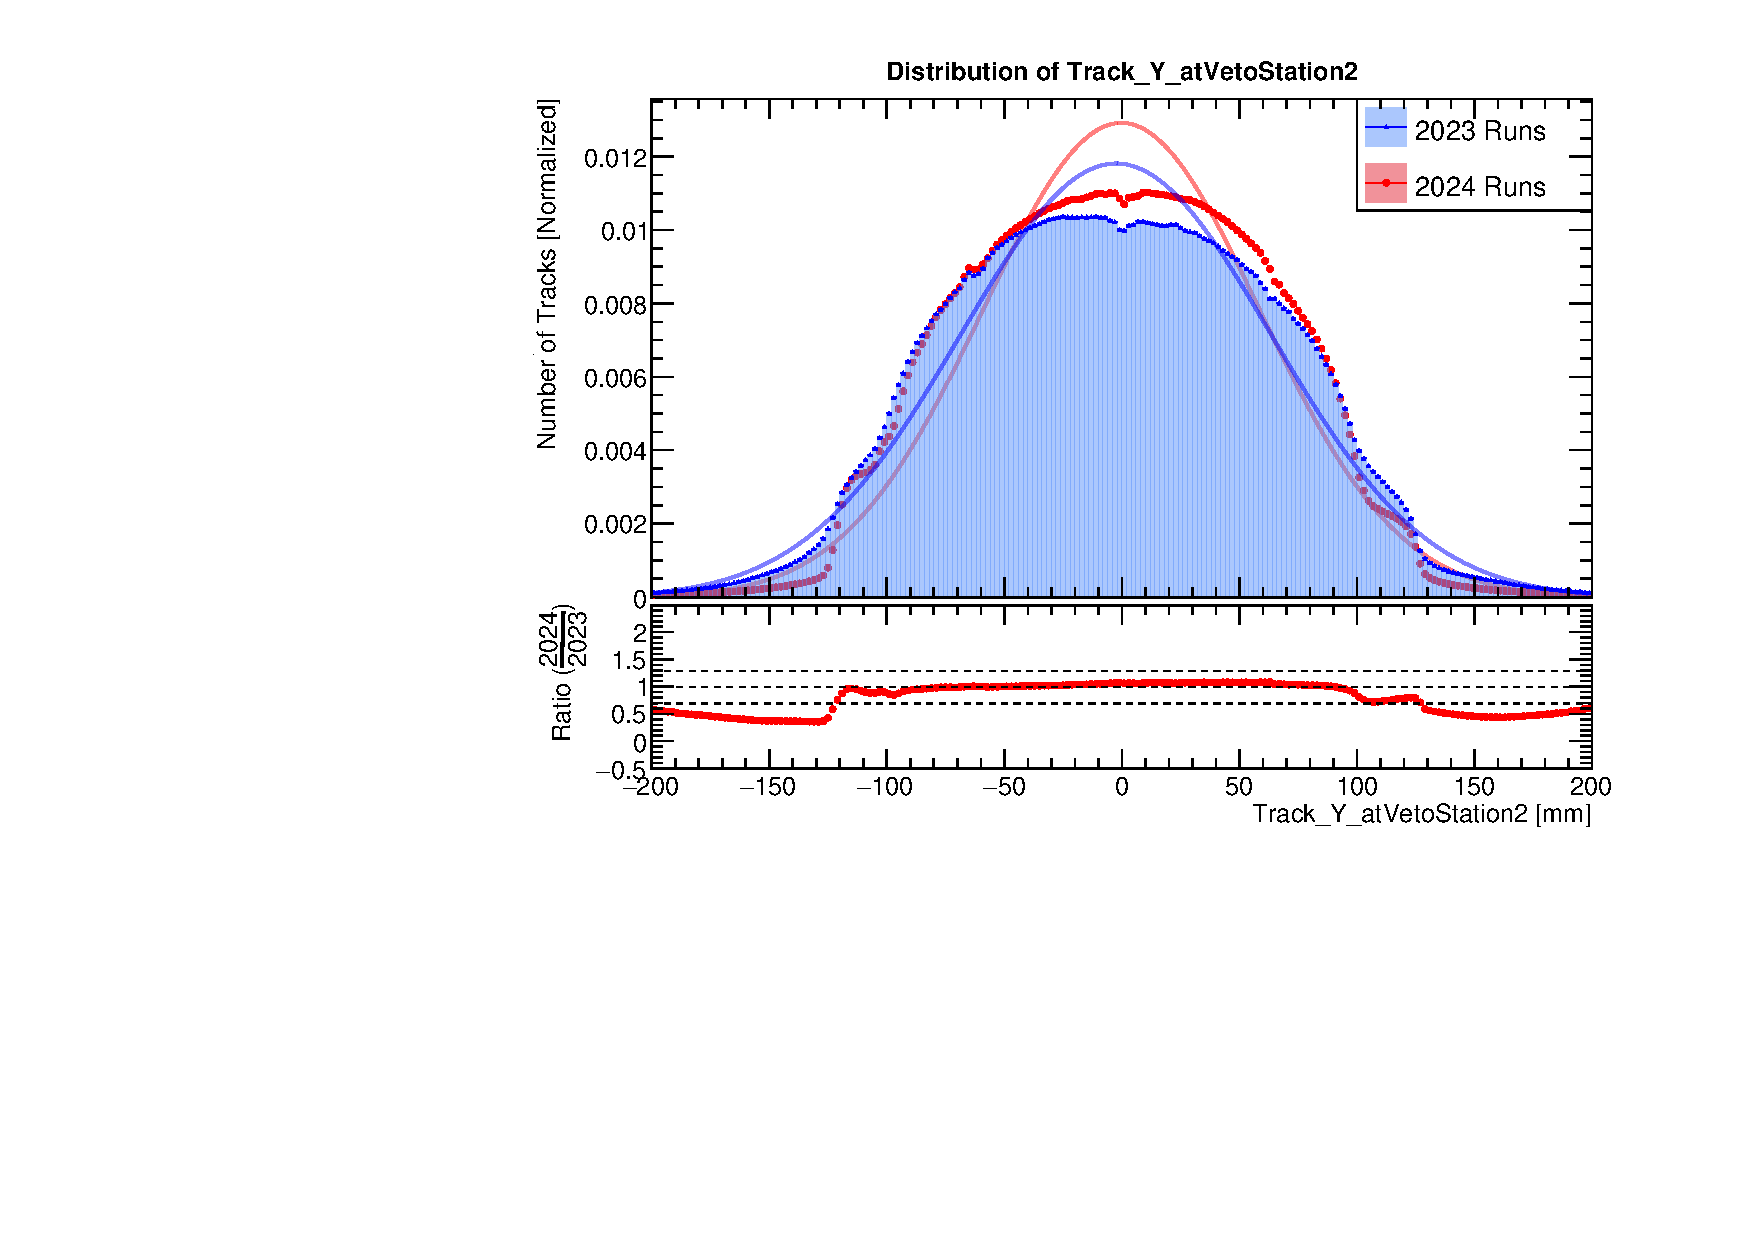
\includegraphics[width=\linewidth] {\plots/Track_Y_atVetoStation2.pdf}
                \caption{Track Position y at Veto Station 2}
            \end{figure}
        \end{column}
    \end{columns}
\end{subframe}

\begin{subframe}{Track Positions at Trigger [SKIP]}
    \begin{columns}
        \begin{column}{0.5\textwidth}
            \begin{figure}
                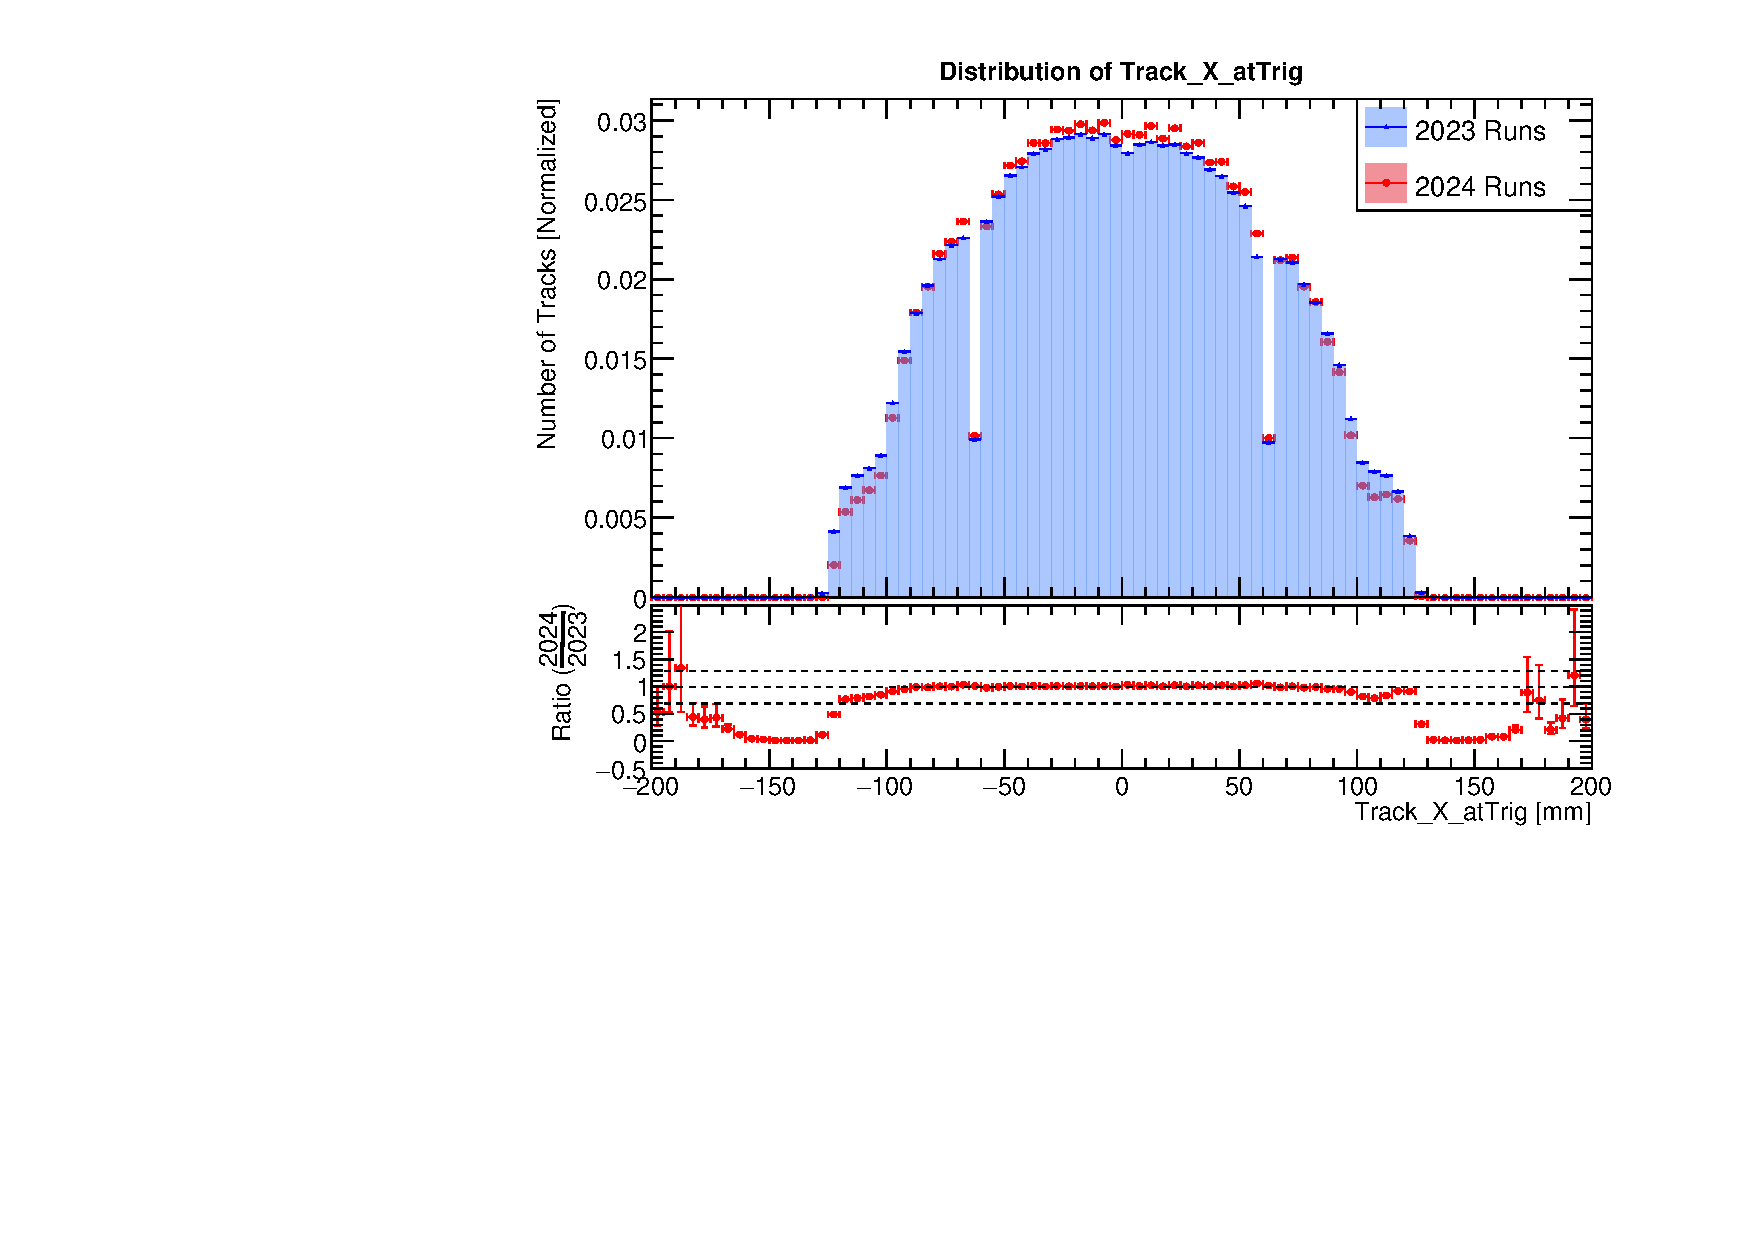
\includegraphics[width=\linewidth] {\plots/Track_X_atTrig.pdf}
                \caption{Track Position x at Trigger/Timing Station}
            \end{figure}
        \end{column}
        \begin{column}{0.5\textwidth}
            \begin{figure}
                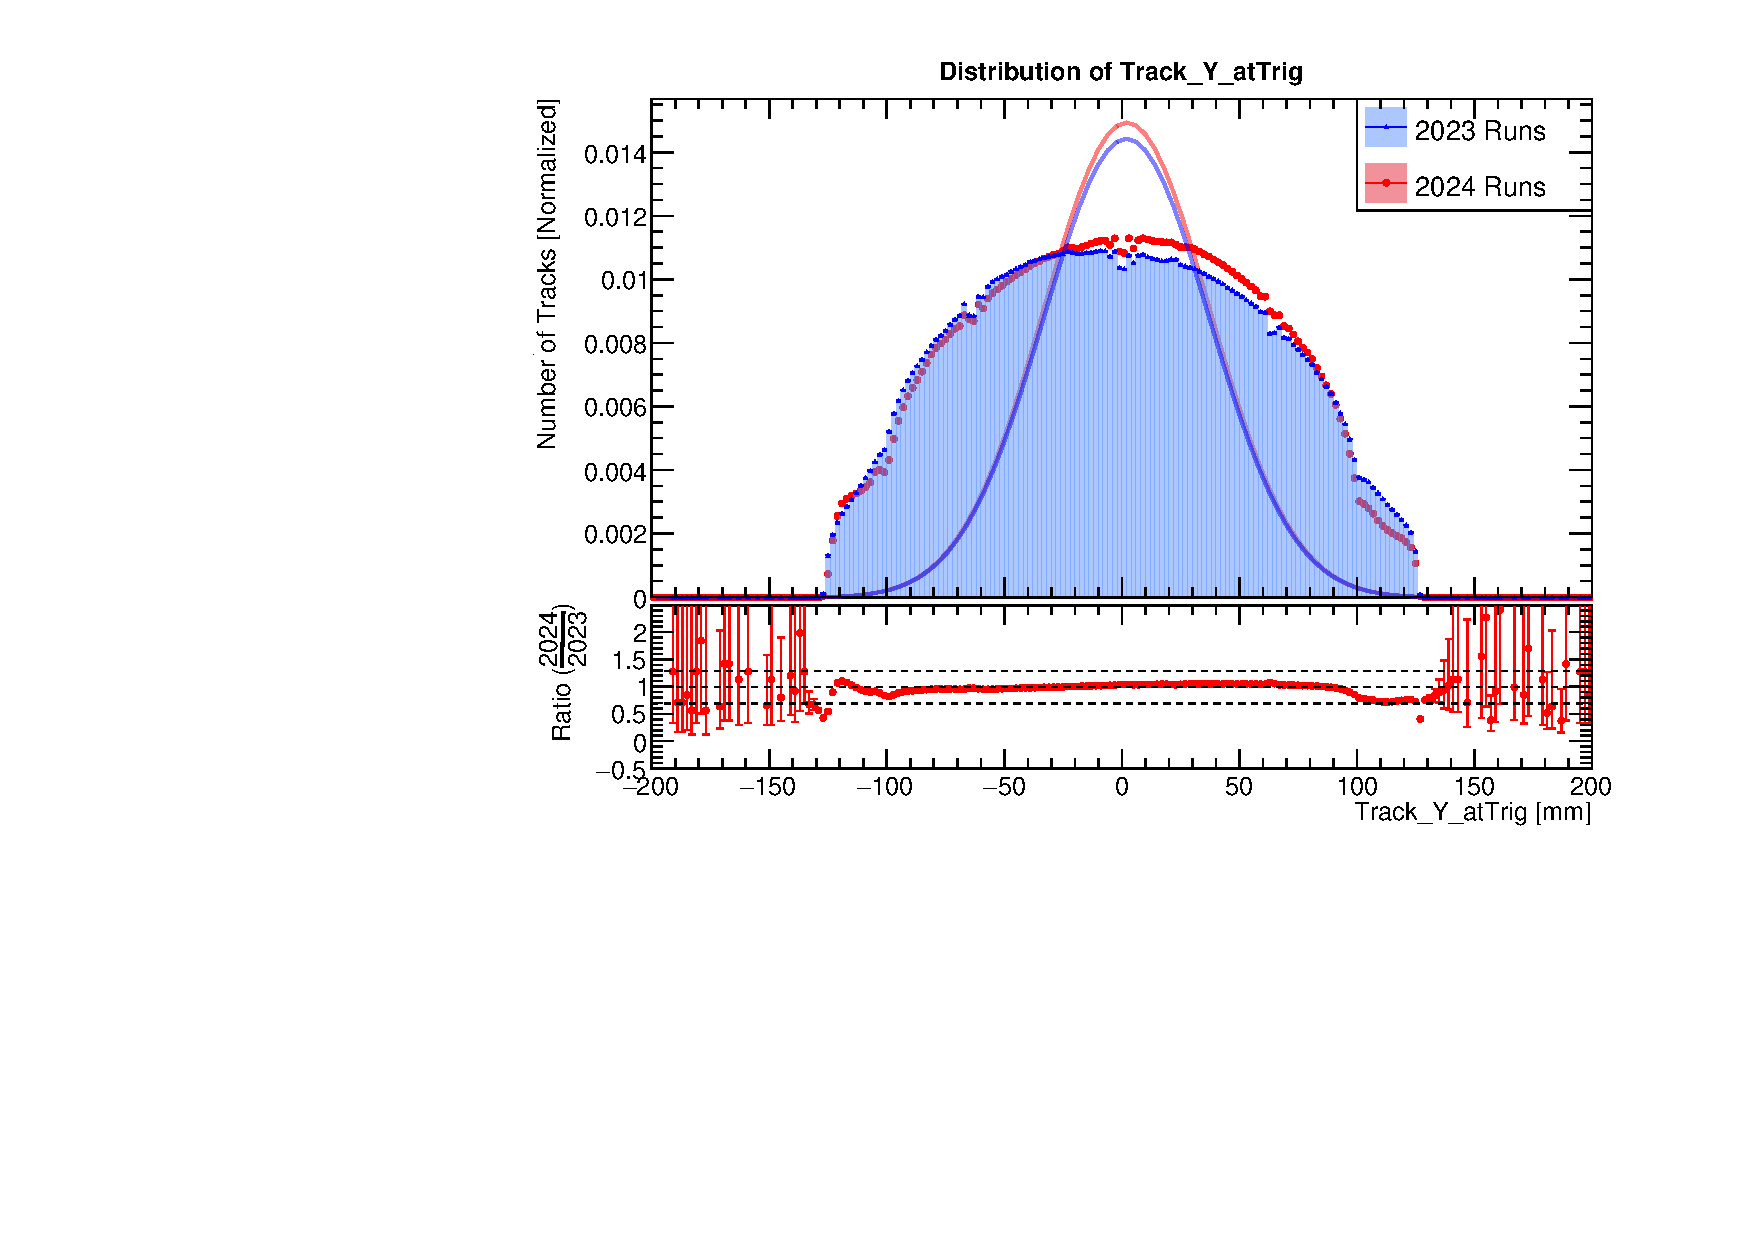
\includegraphics[width=\linewidth] {\plots/Track_Y_atTrig.pdf}
                \caption{Track Position y at Trigger/Timing Station}
            \end{figure}
        \end{column}
    \end{columns}
\end{subframe}

\begin{frame}{Track Positions at Tracking Station 1}
    \begin{columns}
        \begin{column}{0.5\textwidth}
            \begin{figure}
                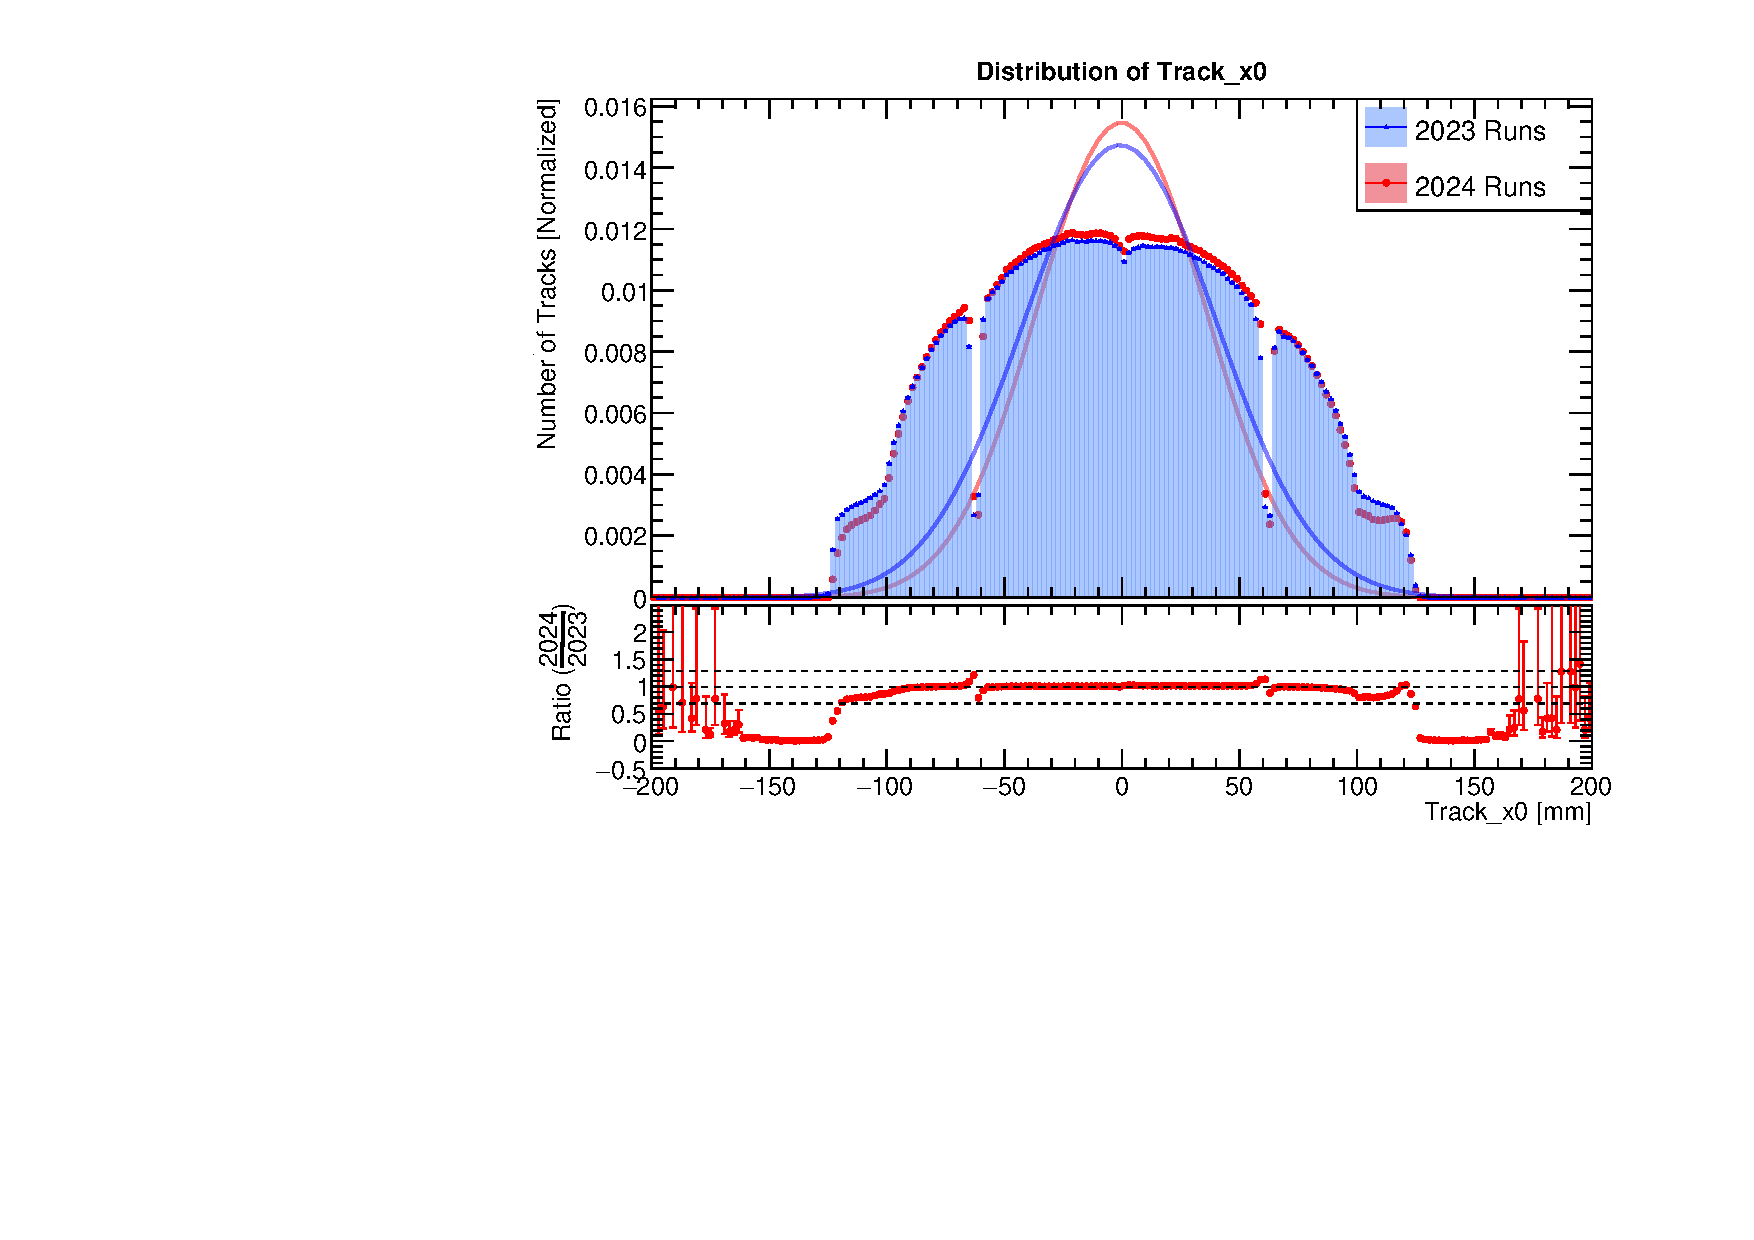
\includegraphics[width=\linewidth] {\plots/Track_x0.pdf}
                \caption{Track Position x at Tracking Station 1}
            \end{figure}
        \end{column}
        \begin{column}{0.5\textwidth}
            \begin{figure}
                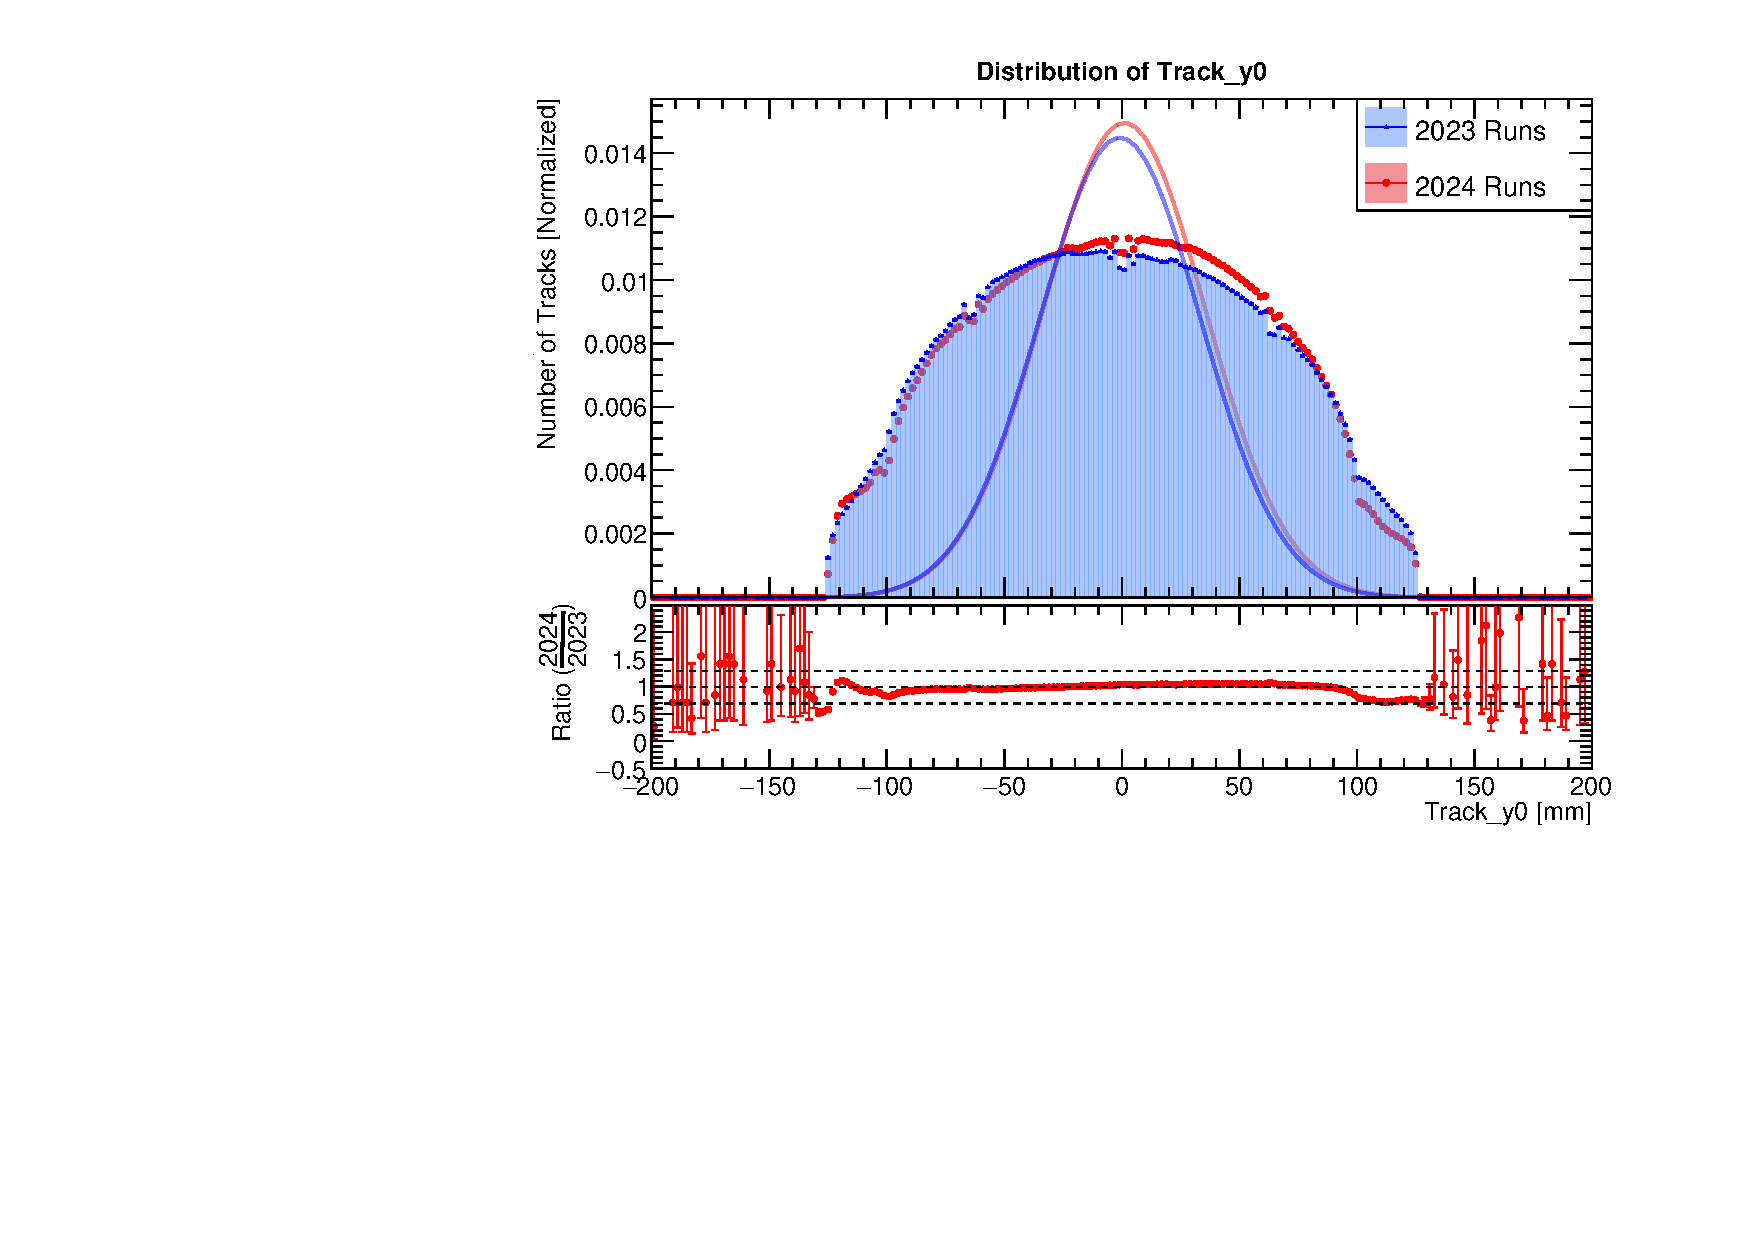
\includegraphics[width=\linewidth] {\plots/Track_y0.pdf}
                \caption{Track Position y at Tracking Station 1}
            \end{figure}
        \end{column}
    \end{columns}
    Only qualitative difference from the VetoNu plots are the sharper peaks here which are from the cut off at 125 mm.
    And the dips in the x-distributions at around 60mm these are from the geometry of the tracking stations.
\end{frame}

\begin{frame}{Track Positions at Tracking Station 2}
    \begin{columns}
        \begin{column}{0.5\textwidth}
            \begin{figure}
                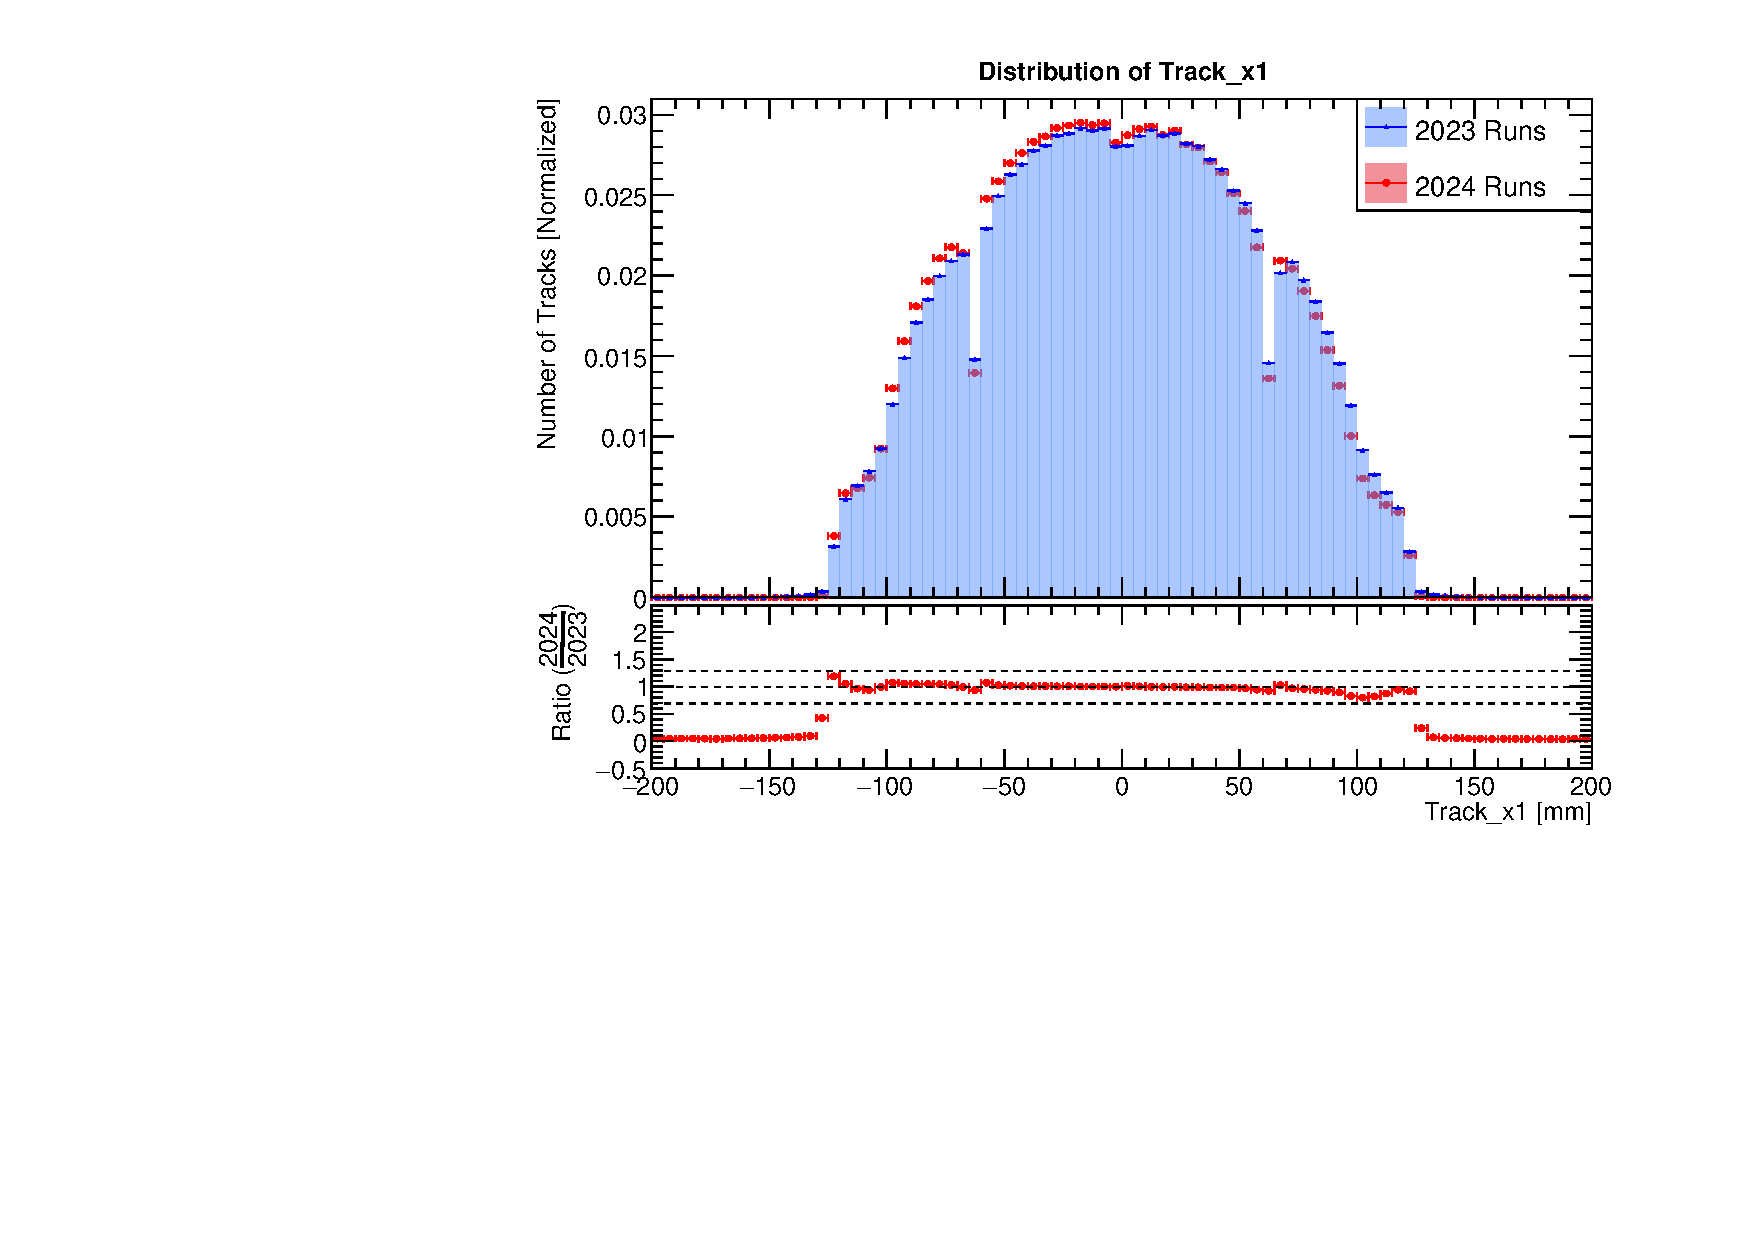
\includegraphics[width=\linewidth] {\plots/Track_x1.pdf}
                \caption{Track Position x at Tracking Station 2}
            \end{figure}
        \end{column}
        \begin{column}{0.5\textwidth}
            \begin{figure}
                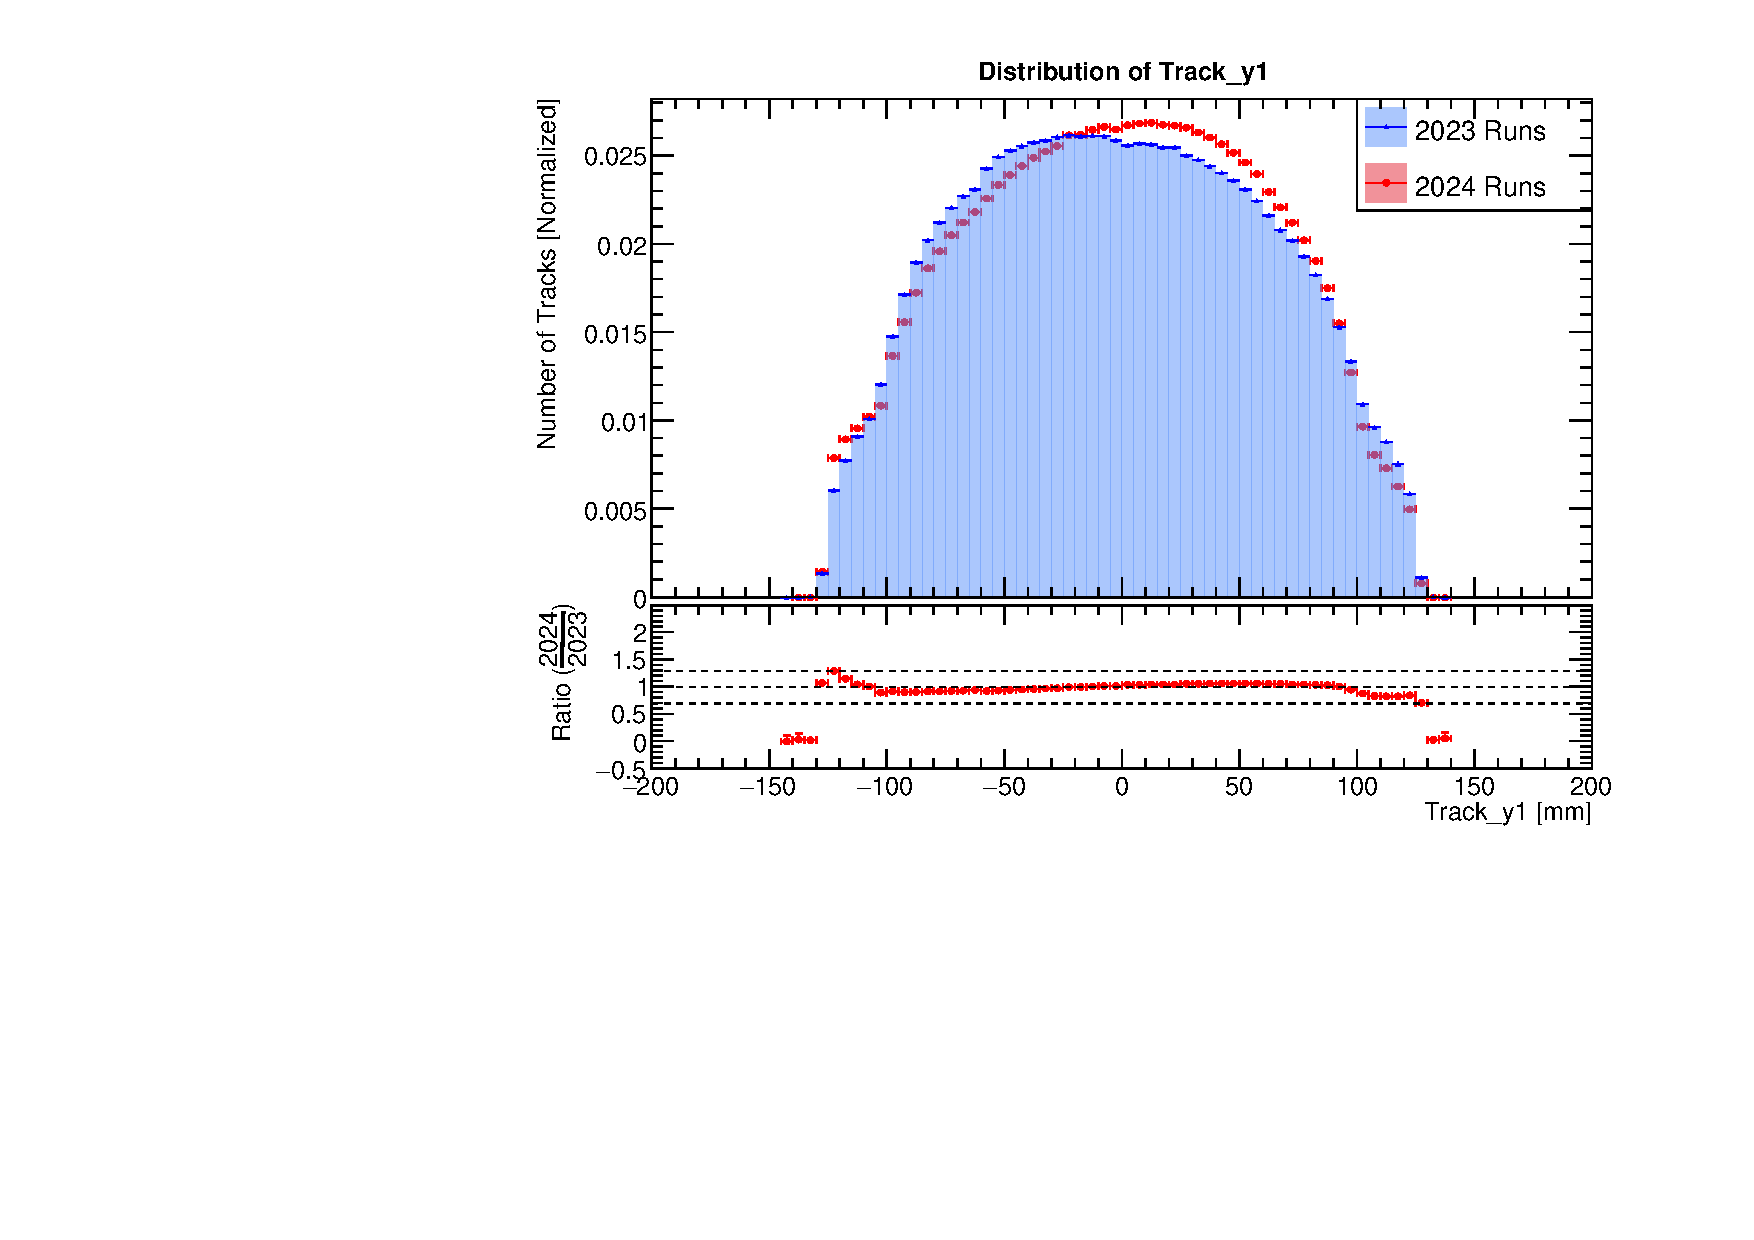
\includegraphics[width=\linewidth] {\plots/Track_y1.pdf}
                \caption{Track Position y at Tracking Station 2}
            \end{figure}
        \end{column}
    \end{columns}
\end{frame}

\begin{subframe}{Track Positions at Preshower 1 [SKIP]}
    \begin{columns}
        \begin{column}{0.5\textwidth}
            \begin{figure}
                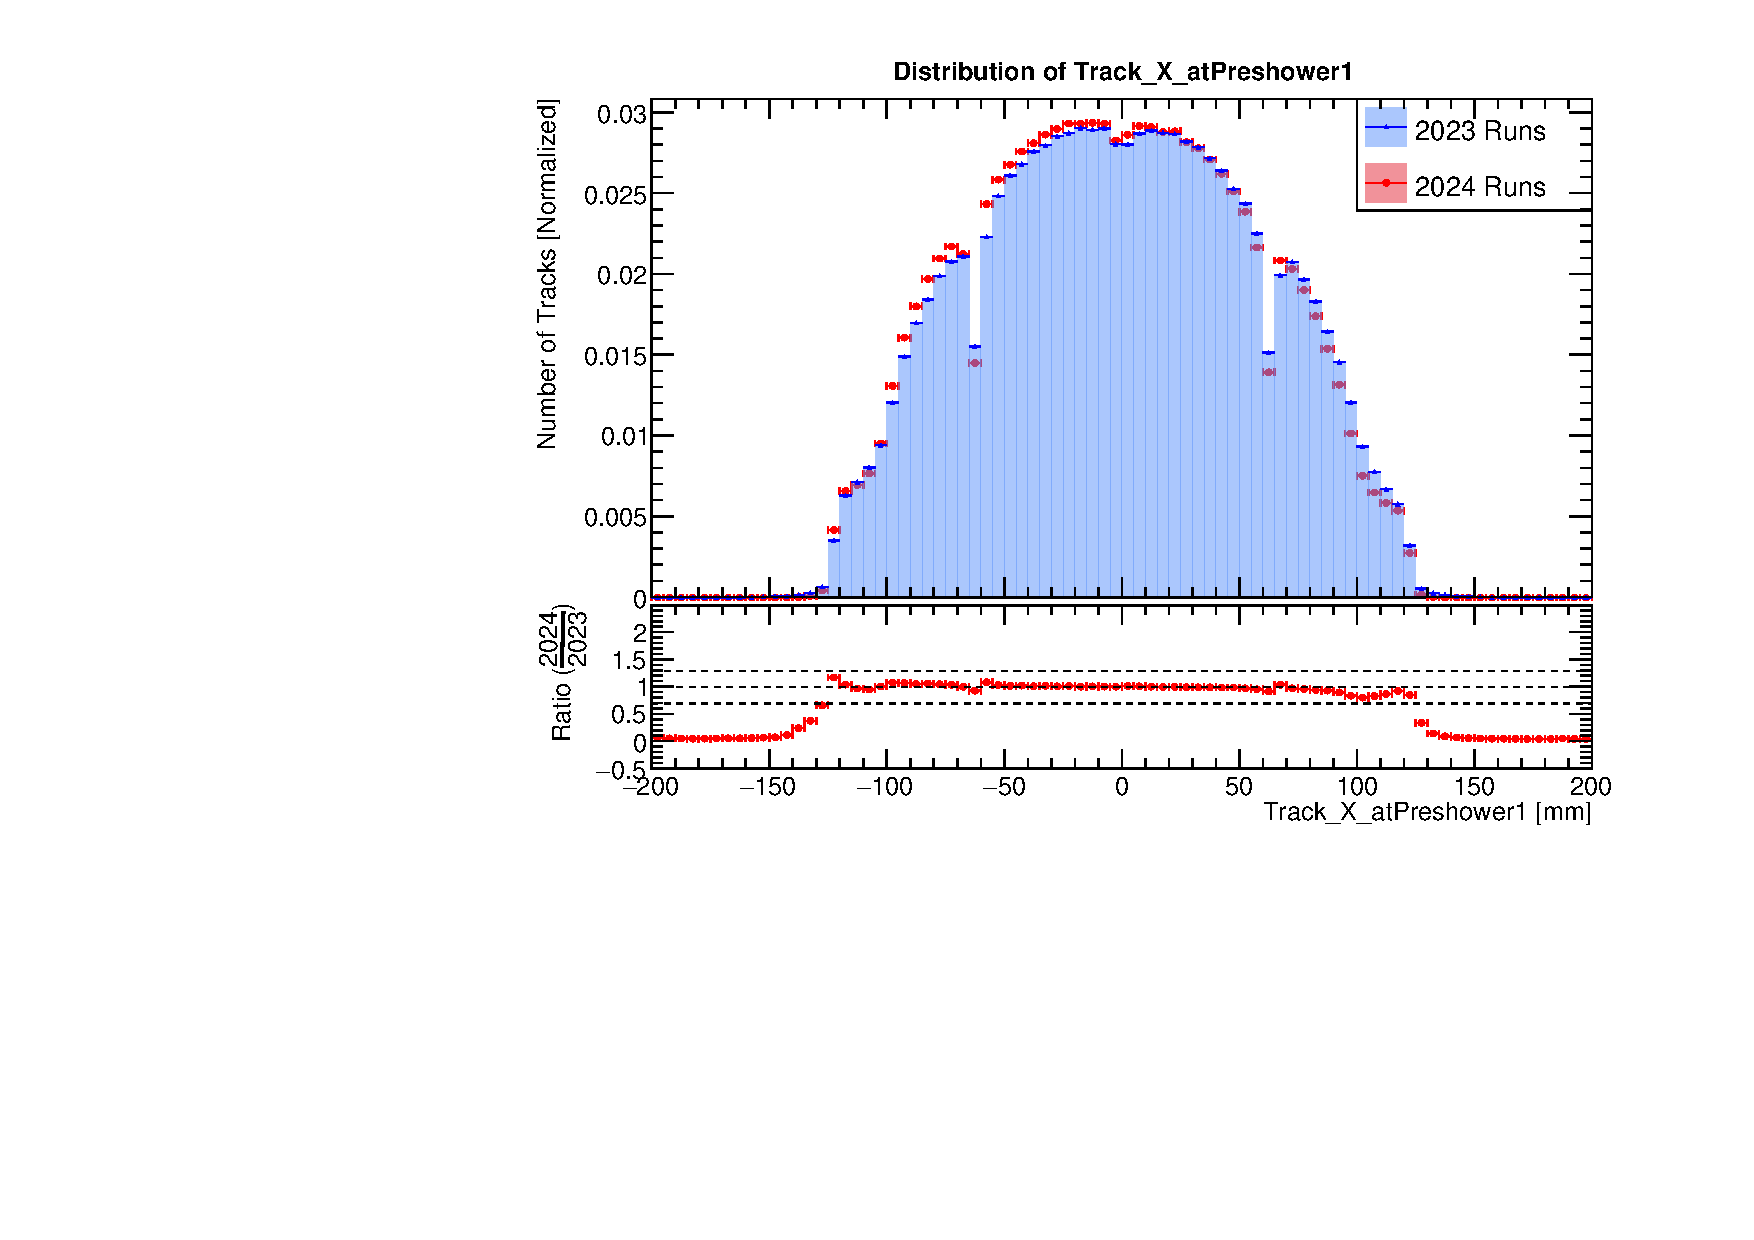
\includegraphics[width=\linewidth] {\plots/Track_X_atPreshower1.pdf}
                \caption{Track Position x at Preshower 1}
            \end{figure}
        \end{column}
        \begin{column}{0.5\textwidth}
            \begin{figure}
                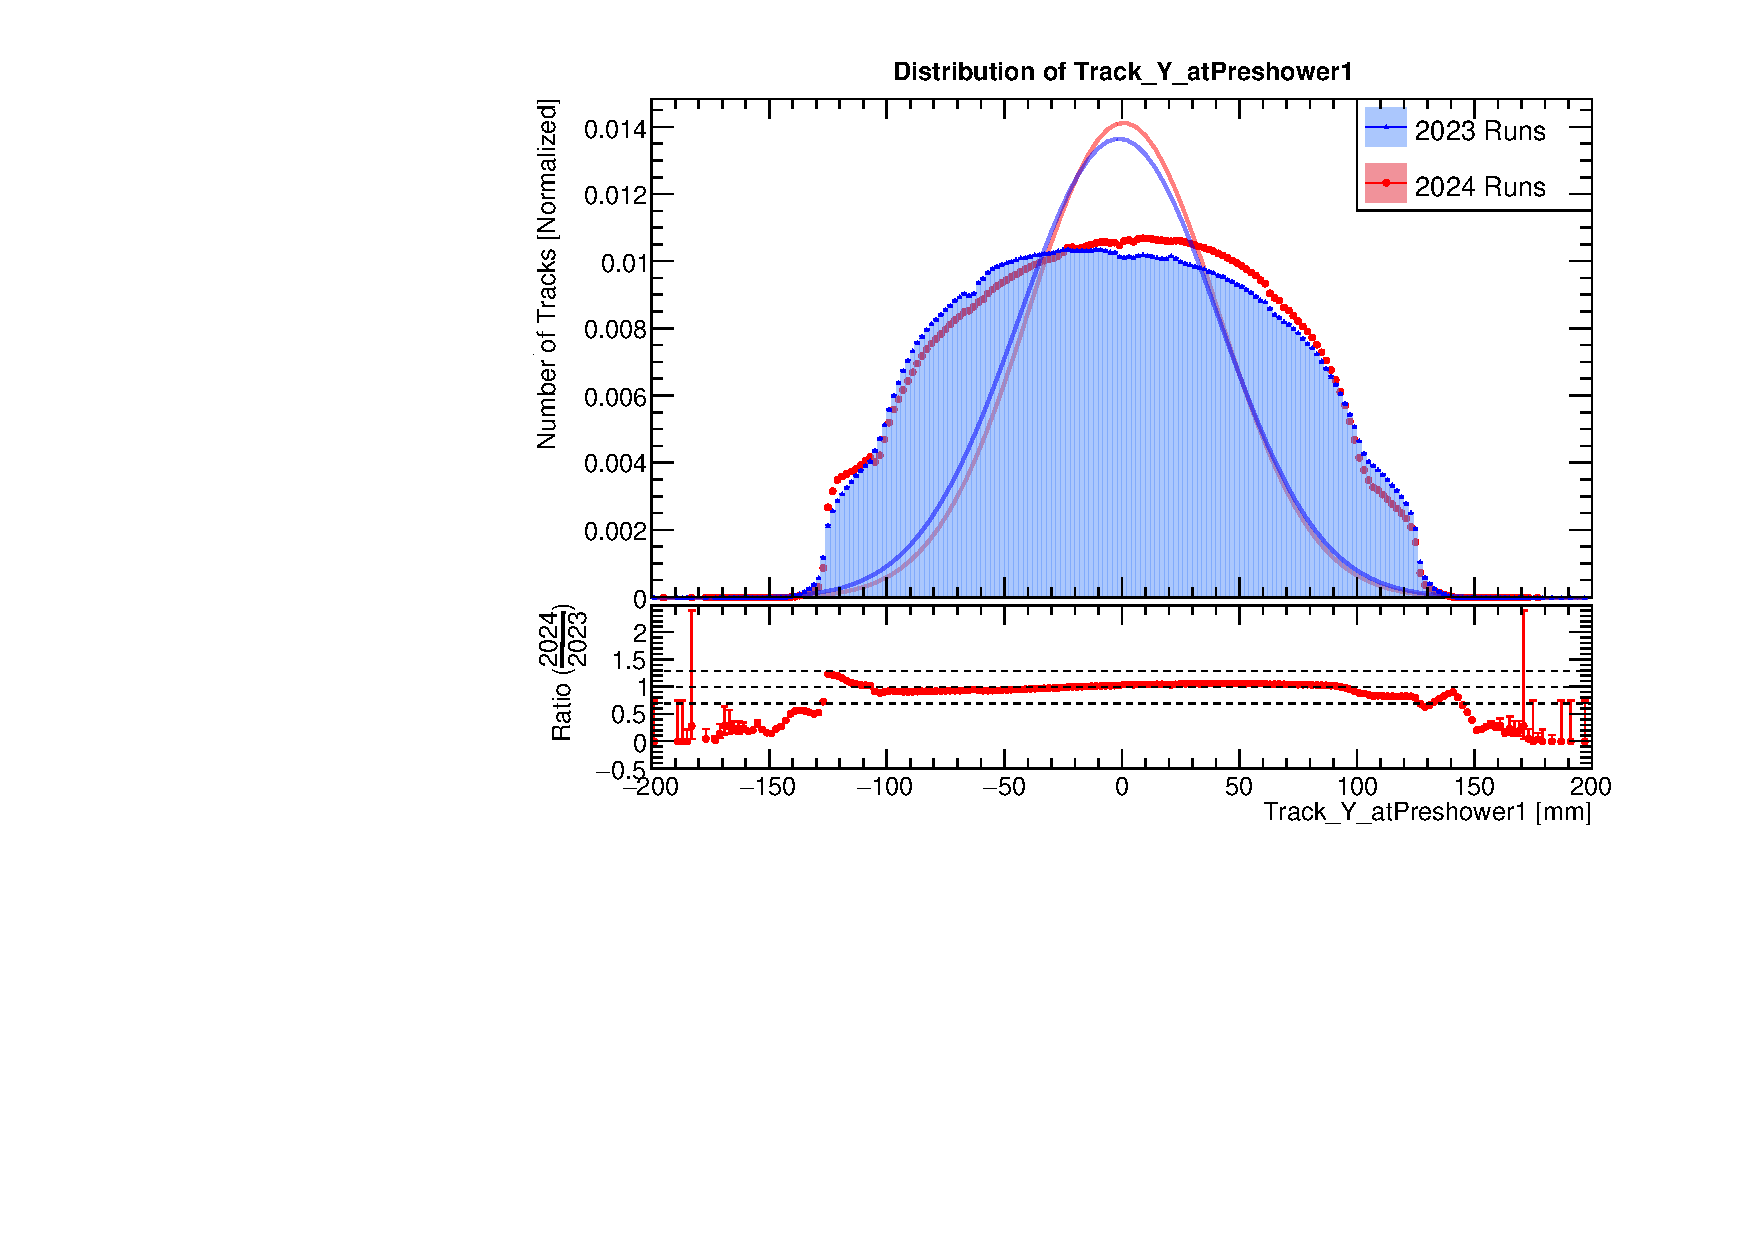
\includegraphics[width=\linewidth] {\plots/Track_Y_atPreshower1.pdf}
                \caption{Track Position y at Preshower 1}
            \end{figure}
        \end{column}
    \end{columns}
\end{subframe}

\begin{subframe}{Track Positions at Preshower 2 [SKIP]}
    \begin{columns}
        \begin{column}{0.5\textwidth}
            \begin{figure}
                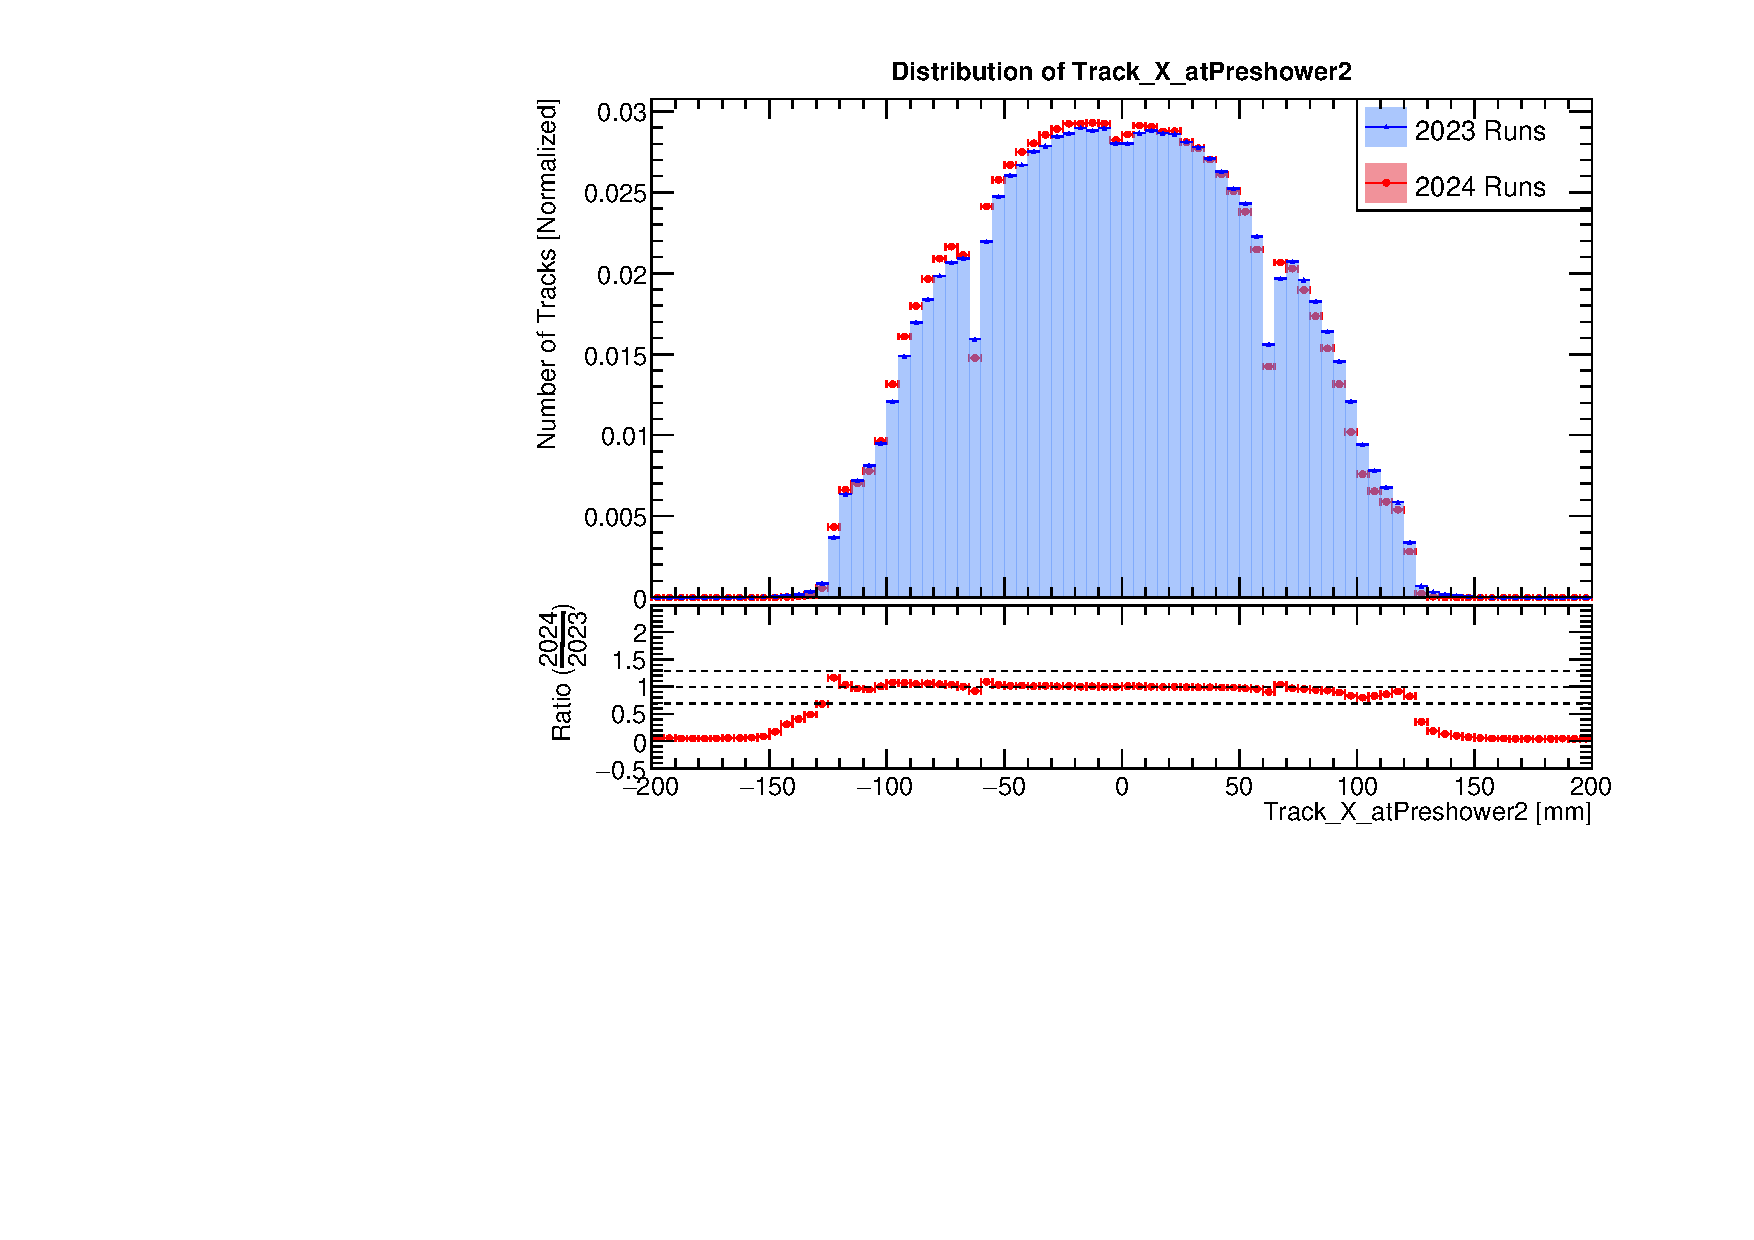
\includegraphics[width=\linewidth] {\plots/Track_X_atPreshower2.pdf}
                \caption{Track Position x at Preshower 2}
            \end{figure}
        \end{column}
        \begin{column}{0.5\textwidth}
            \begin{figure}
                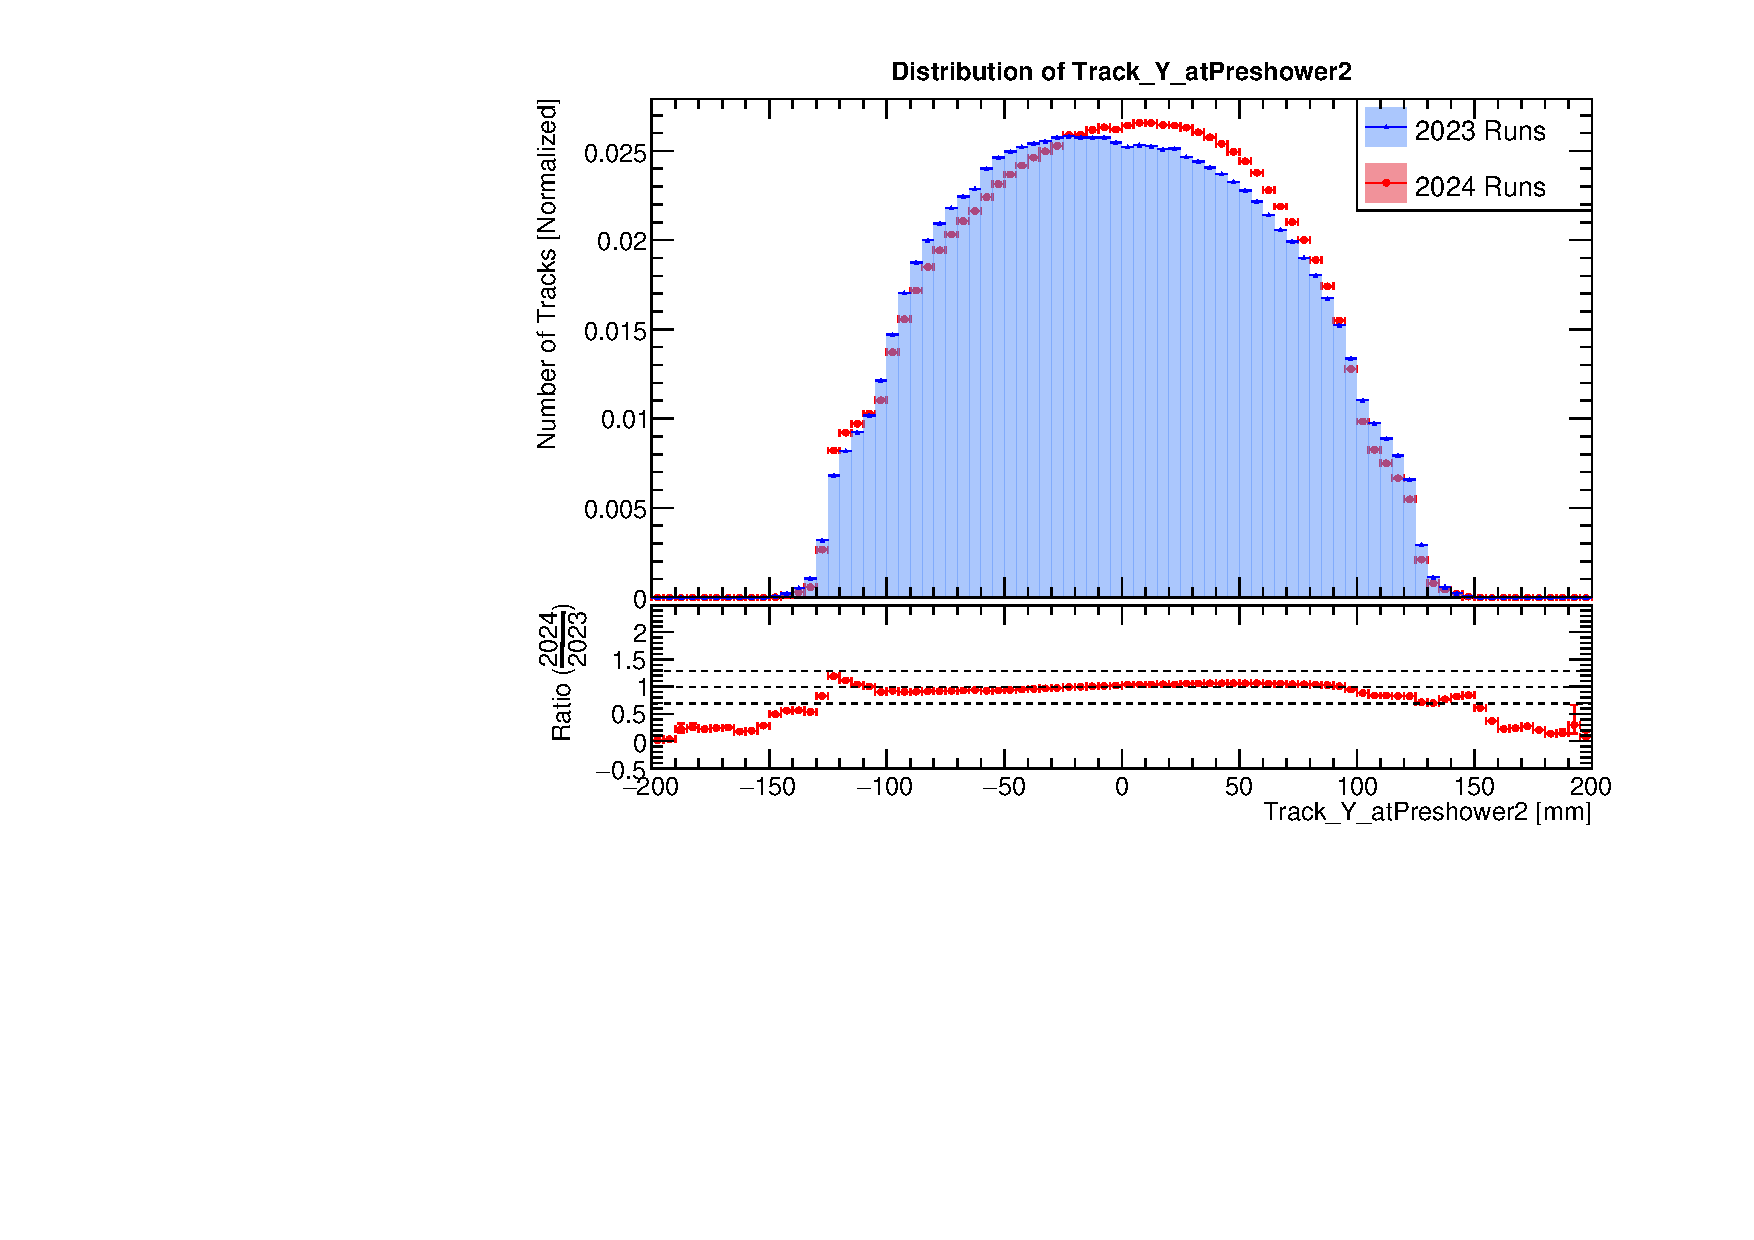
\includegraphics[width=\linewidth] {\plots/Track_Y_atPreshower2.pdf}
                \caption{Track Position y at Preshower 2}
            \end{figure}
        \end{column}
    \end{columns}
\end{subframe}

\begin{frame}{Track Positions at Calo}
    \begin{columns}
        \begin{column}{0.5\textwidth}
            \begin{figure}
                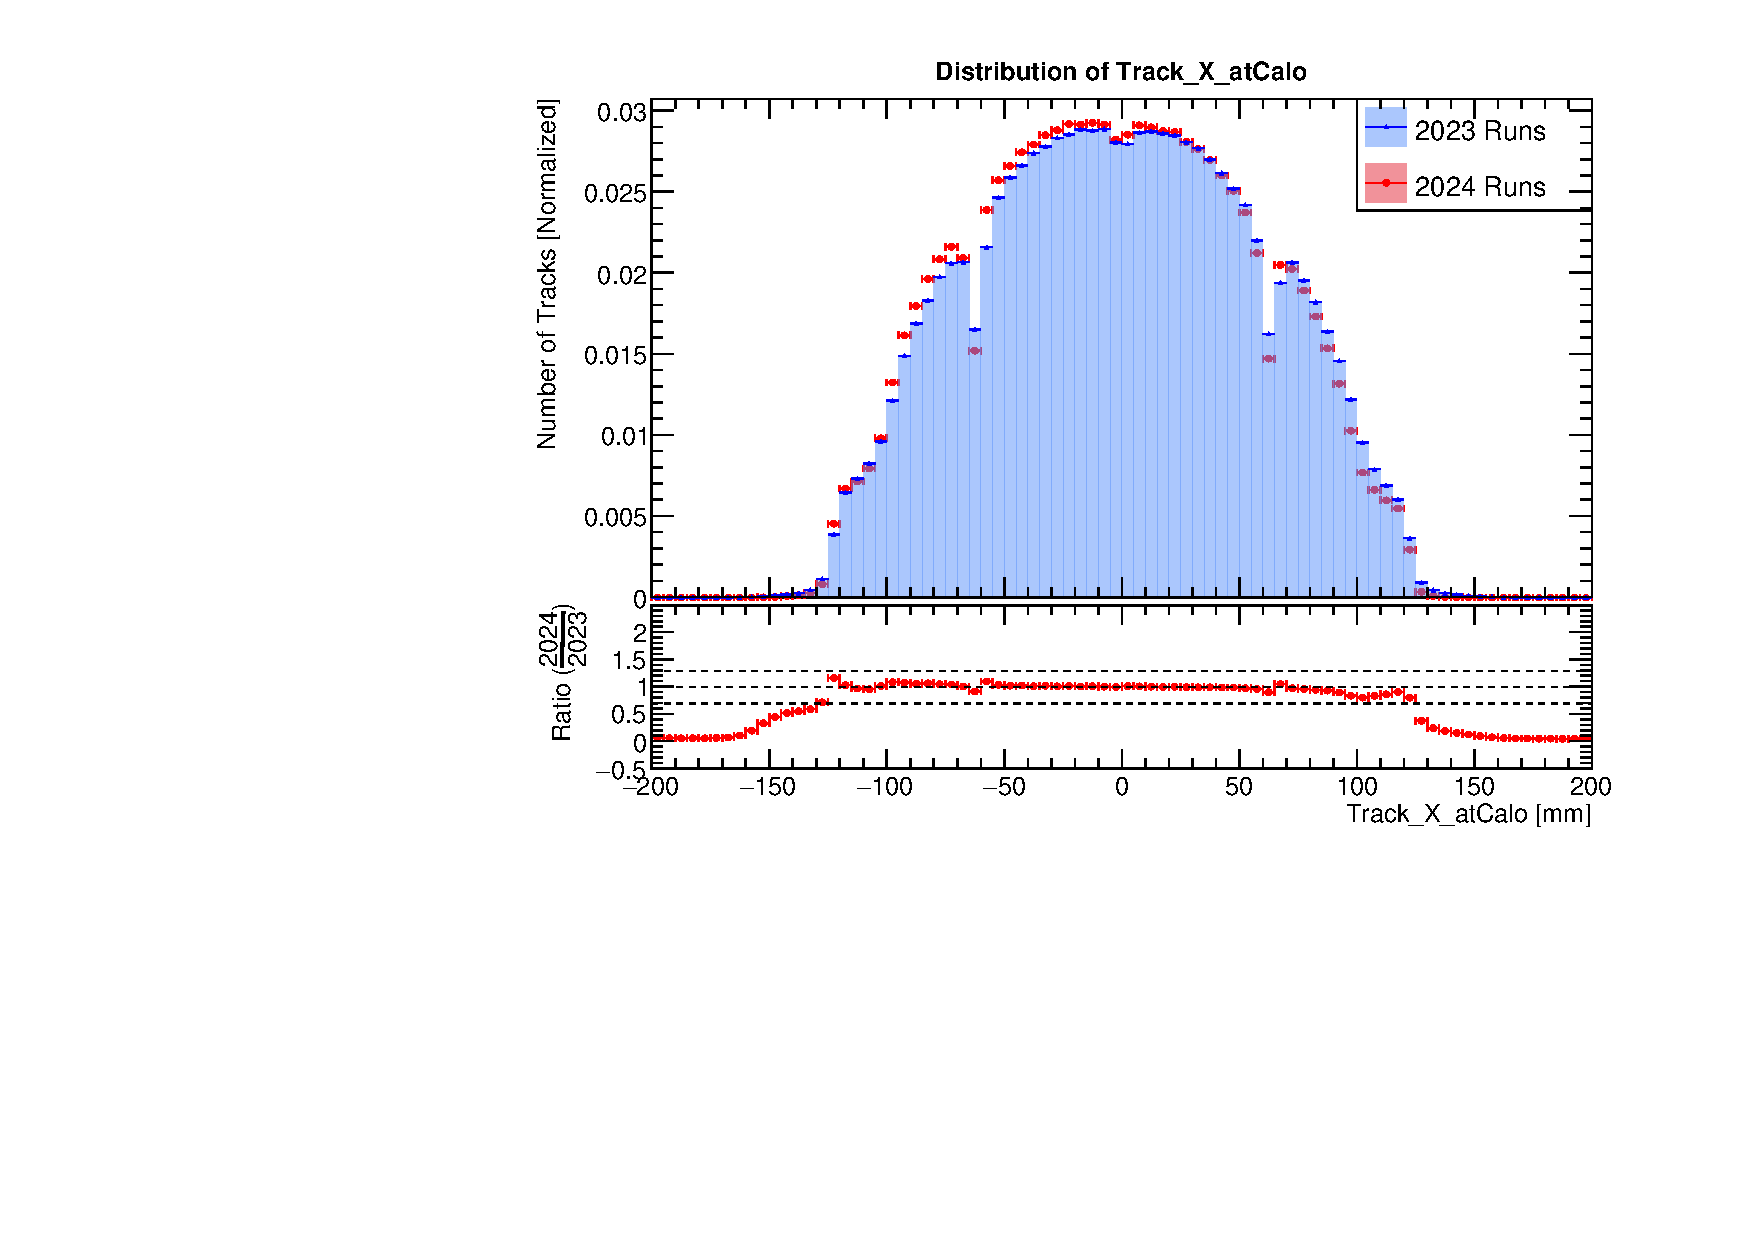
\includegraphics[width=\linewidth] {\plots/Track_X_atCalo.pdf}
                \caption{Track Position x at Calo}
            \end{figure}
        \end{column}
        \begin{column}{0.5\textwidth}
            \begin{figure}
                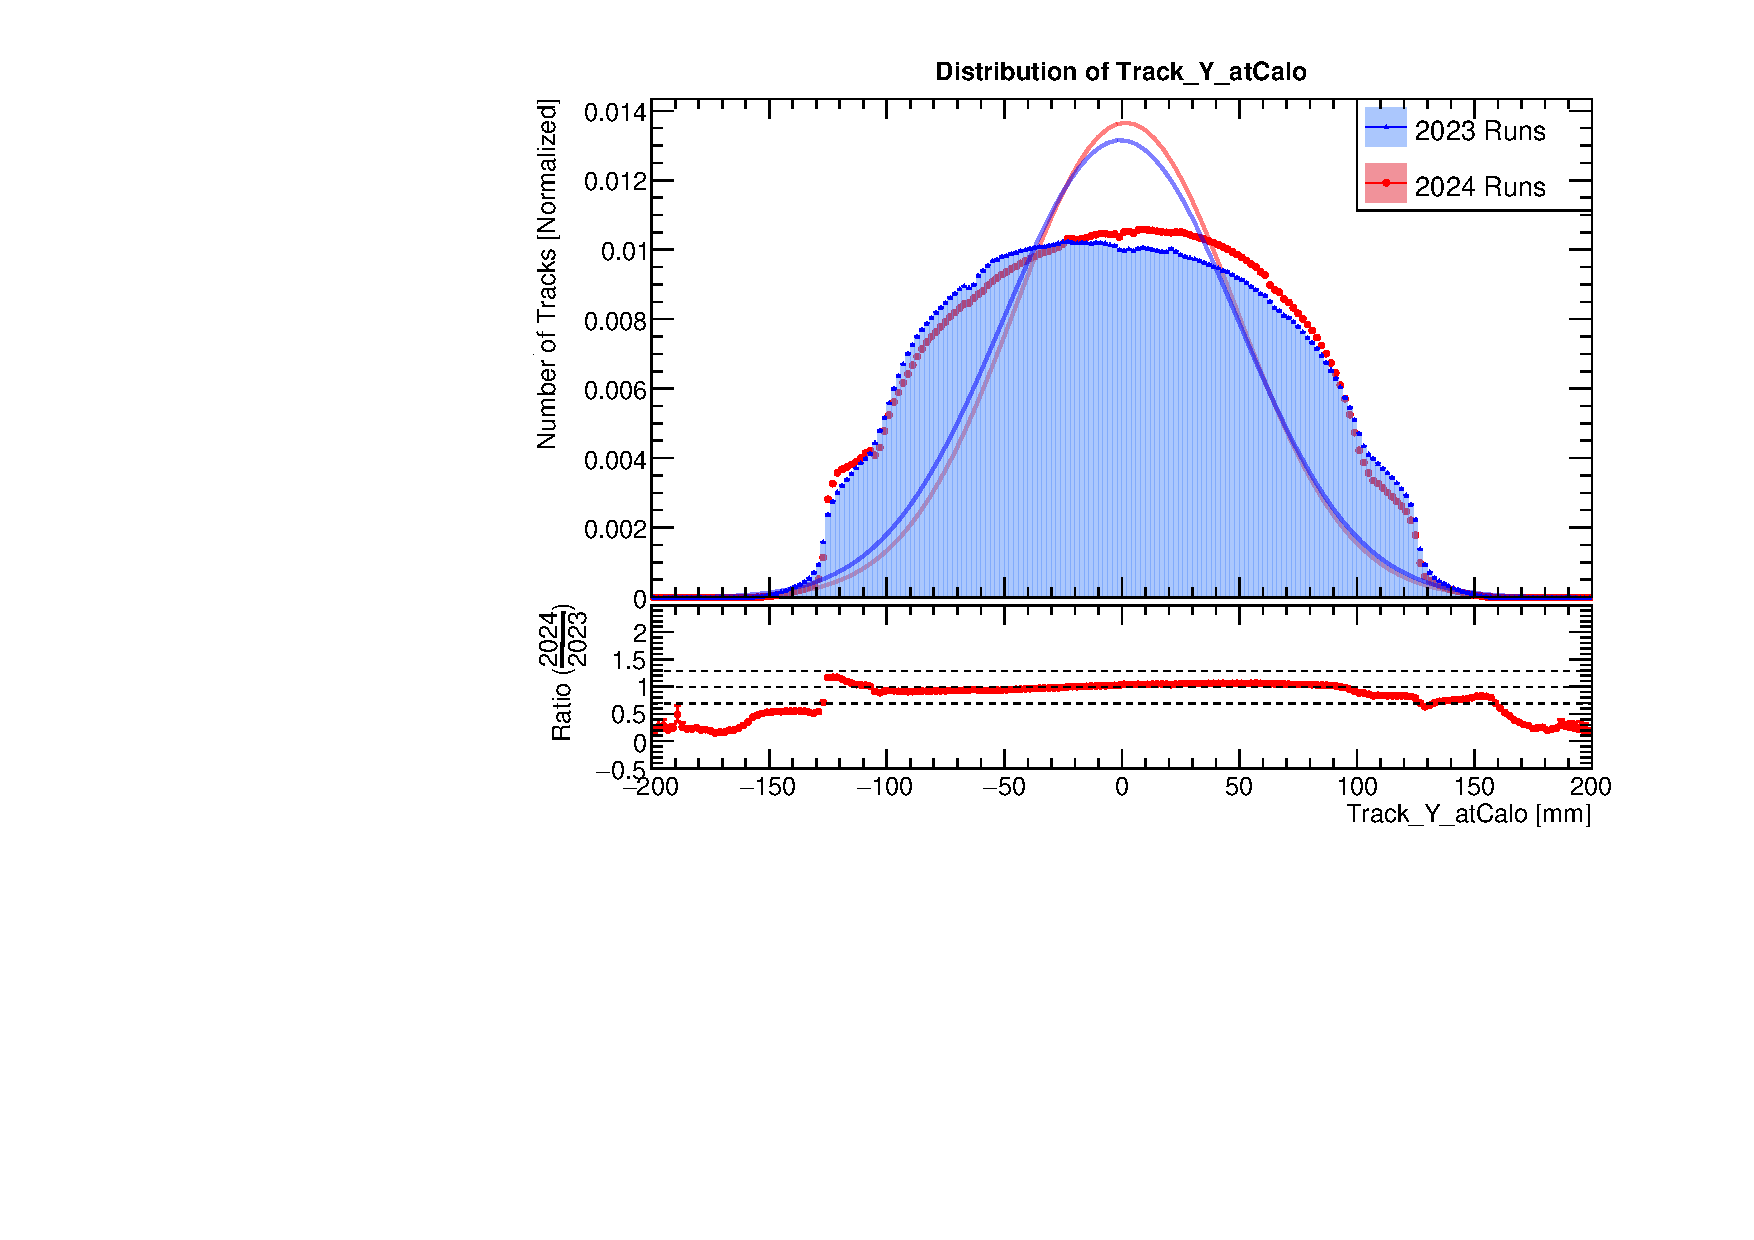
\includegraphics[width=\linewidth] {\plots/Track_Y_atCalo.pdf}
                \caption{Track Position y at Calo}
            \end{figure}
        \end{column}
    \end{columns}
\end{frame}

\begin{frame}{Track Positions at Max Radius}
    \begin{columns}
        \begin{column}{0.5\textwidth}
            \begin{figure}
                \includegraphics[width=\linewidth] {\plots/Track_X_atMaxRadius.pdf}
                \caption{}
            \end{figure}
        \end{column}
        \begin{column}{0.5\textwidth}
            \begin{figure}
                \includegraphics[width=\linewidth] {\plots/Track_Y_atMaxRadius.pdf}
                \caption{}
            \end{figure}
        \end{column}
    \end{columns}
\end{frame}
\begin{frame}{Track Angle (\(\theta_x\), \(\theta_y \) ) at Various Stations}
	\begin{itemize}
		\item Vetonu
		\item VetoStation 1 [in Backup]
		\item VetoStation 2 [in Backup]
		\item Trigger/Timing Station [in Backup]
		\item Tracking Station 1
		% \item Tracking Station 1 - z-Momentum 
		\item Tracking Station 3
		\item Preshower 1 [in Backup]
		\item Preshower 2 [in Backup]
		\item Calo
		\item Track Momenta at Station 1
	\end{itemize}
	Note: Track angles defined as \( \theta_x = \arctan\frac{p_x}{p_z}\) and \( \theta_y = \arctan\frac{p_y}{p_z}\)
\end{frame}

\begin{frame}{Track Momenta at VetoNu}
	\begin{columns}
		\begin{column}{0.5\textwidth}
			\begin{figure}
				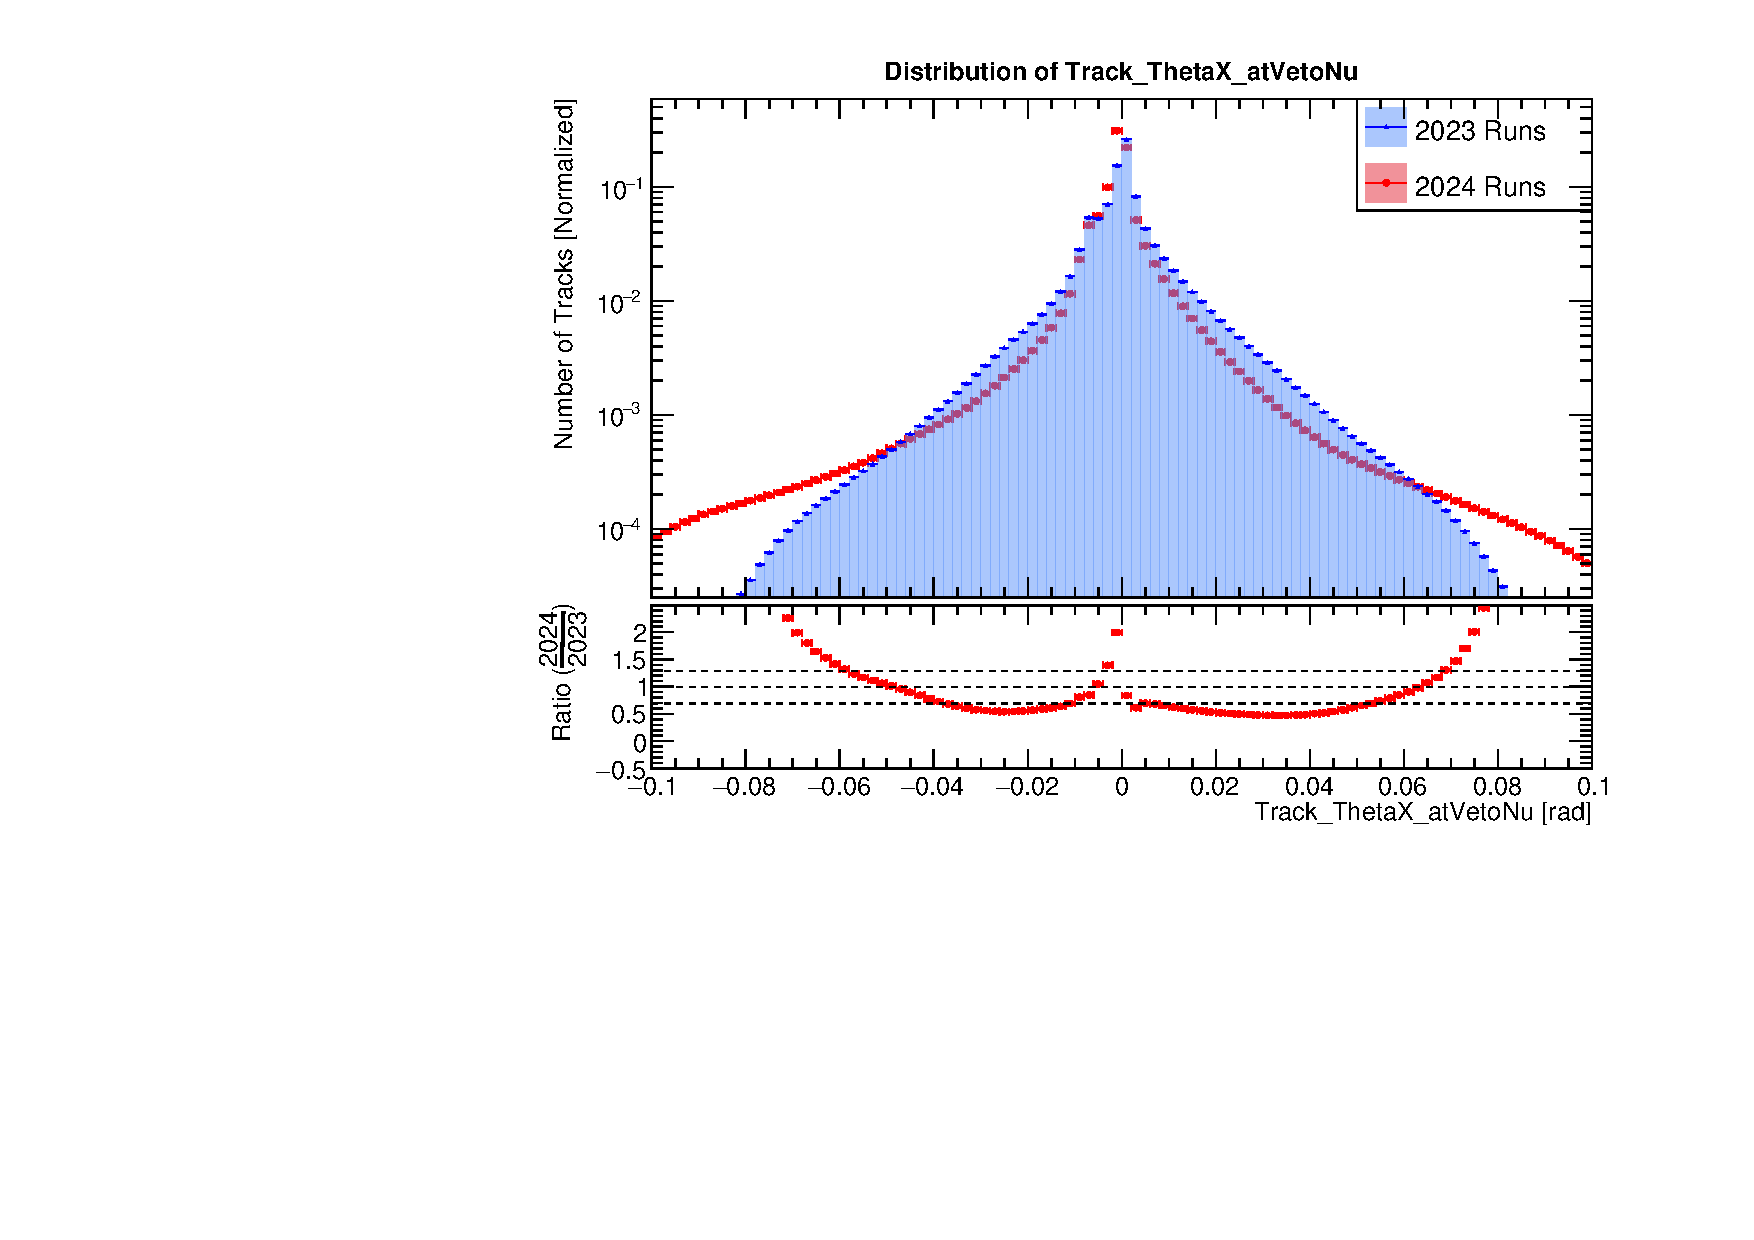
\includegraphics[width=\linewidth] {\plots/Track_ThetaX_atVetoNu.pdf}
				\caption{Track ThetaX at VetoNu}
			\end{figure}
		\end{column}
		\begin{column}{0.5\textwidth}
			\begin{figure}
				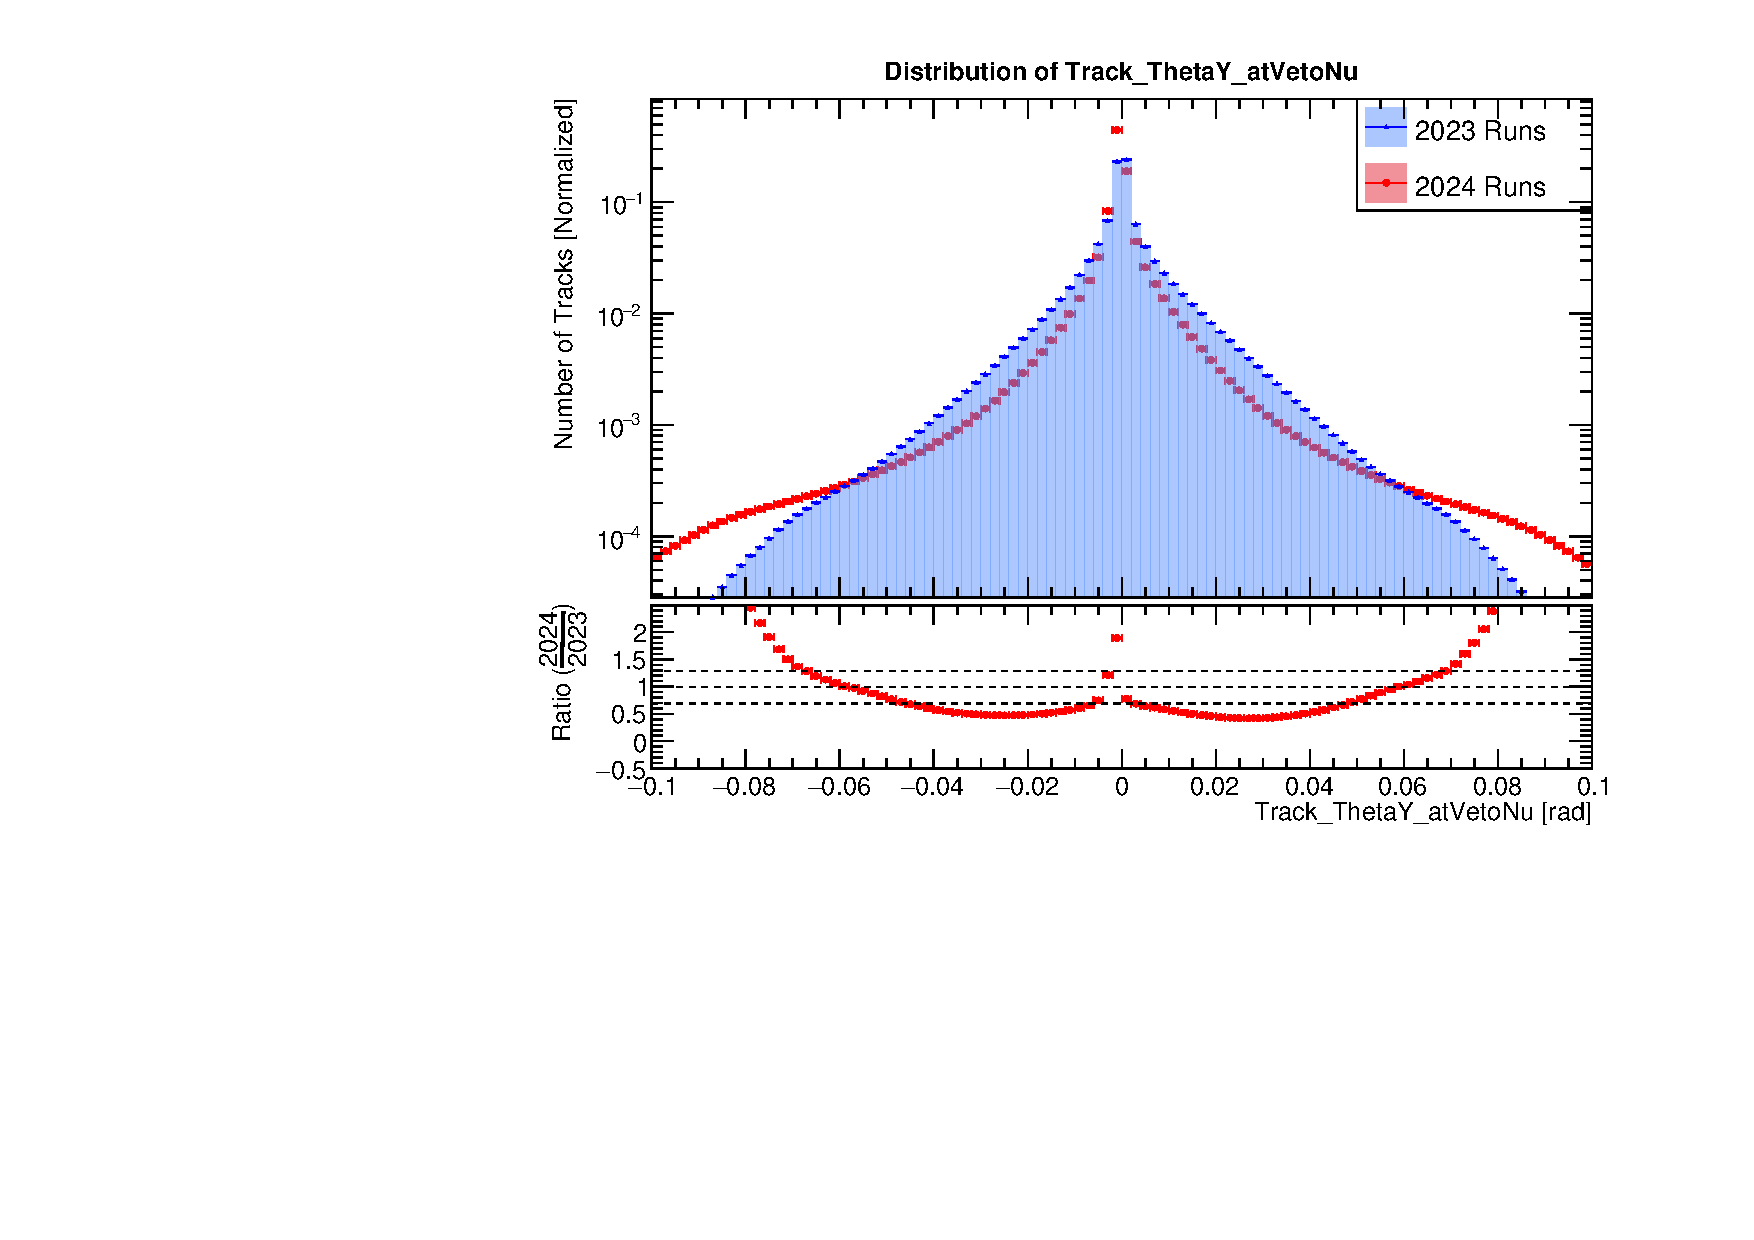
\includegraphics[width=\linewidth] {\plots/Track_ThetaY_atVetoNu.pdf}
				\caption{Track ThetaY at VetoNu}
			\end{figure}
		\end{column}
	\end{columns}
	\begin{itemize}
		\item Needs investigation to understand why the difference
	\end{itemize}
\end{frame}

\begin{subframe}{Track Momenta at VetoStation 1 [SKIP]}
	\begin{columns}
		\begin{column}{0.5\textwidth}
			\begin{figure}
				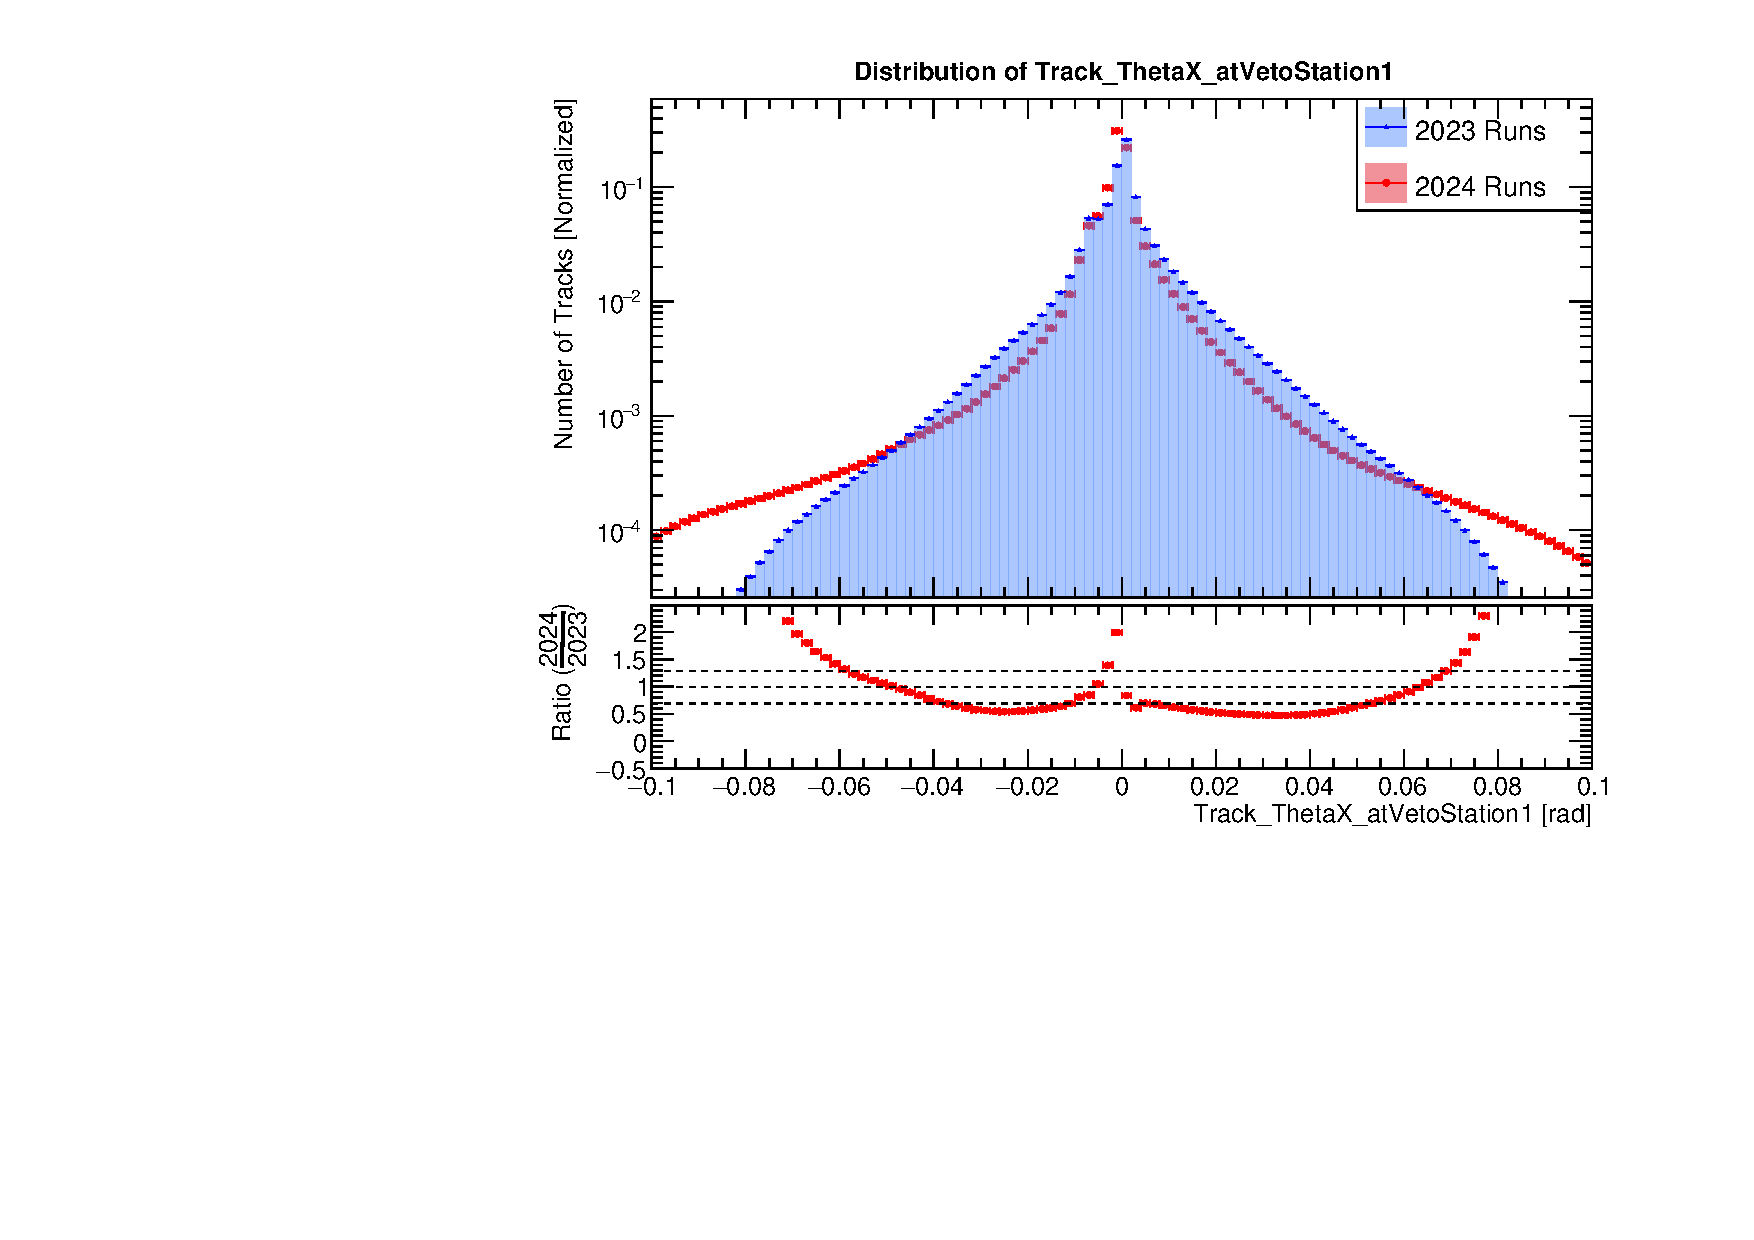
\includegraphics[width=\linewidth] {\plots/Track_ThetaX_atVetoStation1.pdf}
				\caption{Track ThetaX at atVetoStation 1}
			\end{figure}
		\end{column}
		\begin{column}{0.5\textwidth}
			\begin{figure}
				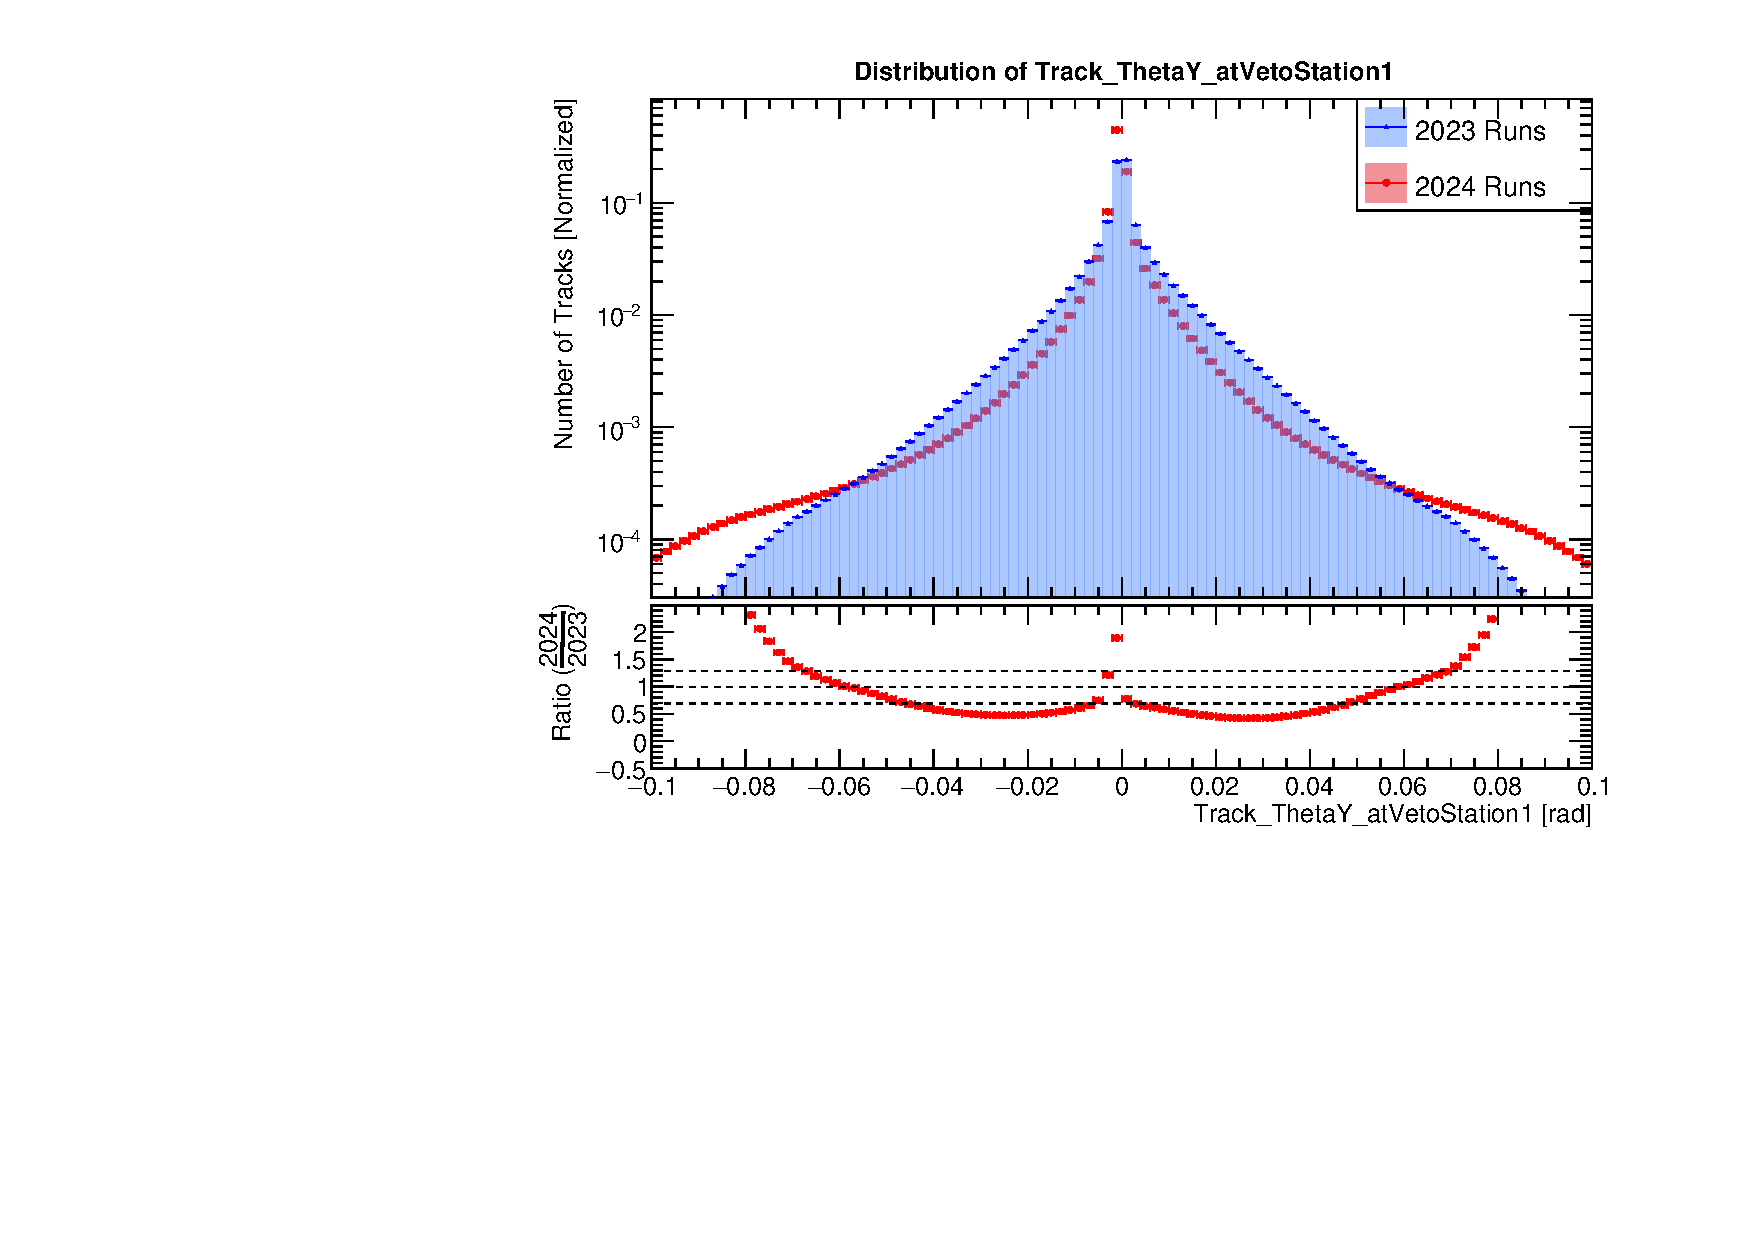
\includegraphics[width=\linewidth] {\plots/Track_ThetaY_atVetoStation1.pdf}
				\caption{Track ThetaY at VetoStation 1}
			\end{figure}
		\end{column}
	\end{columns}
\end{subframe}

\begin{subframe}{Track Angles at VetoStation 2 [SKIP]}
	\begin{columns}
		\begin{column}{0.5\textwidth}
			\begin{figure}
				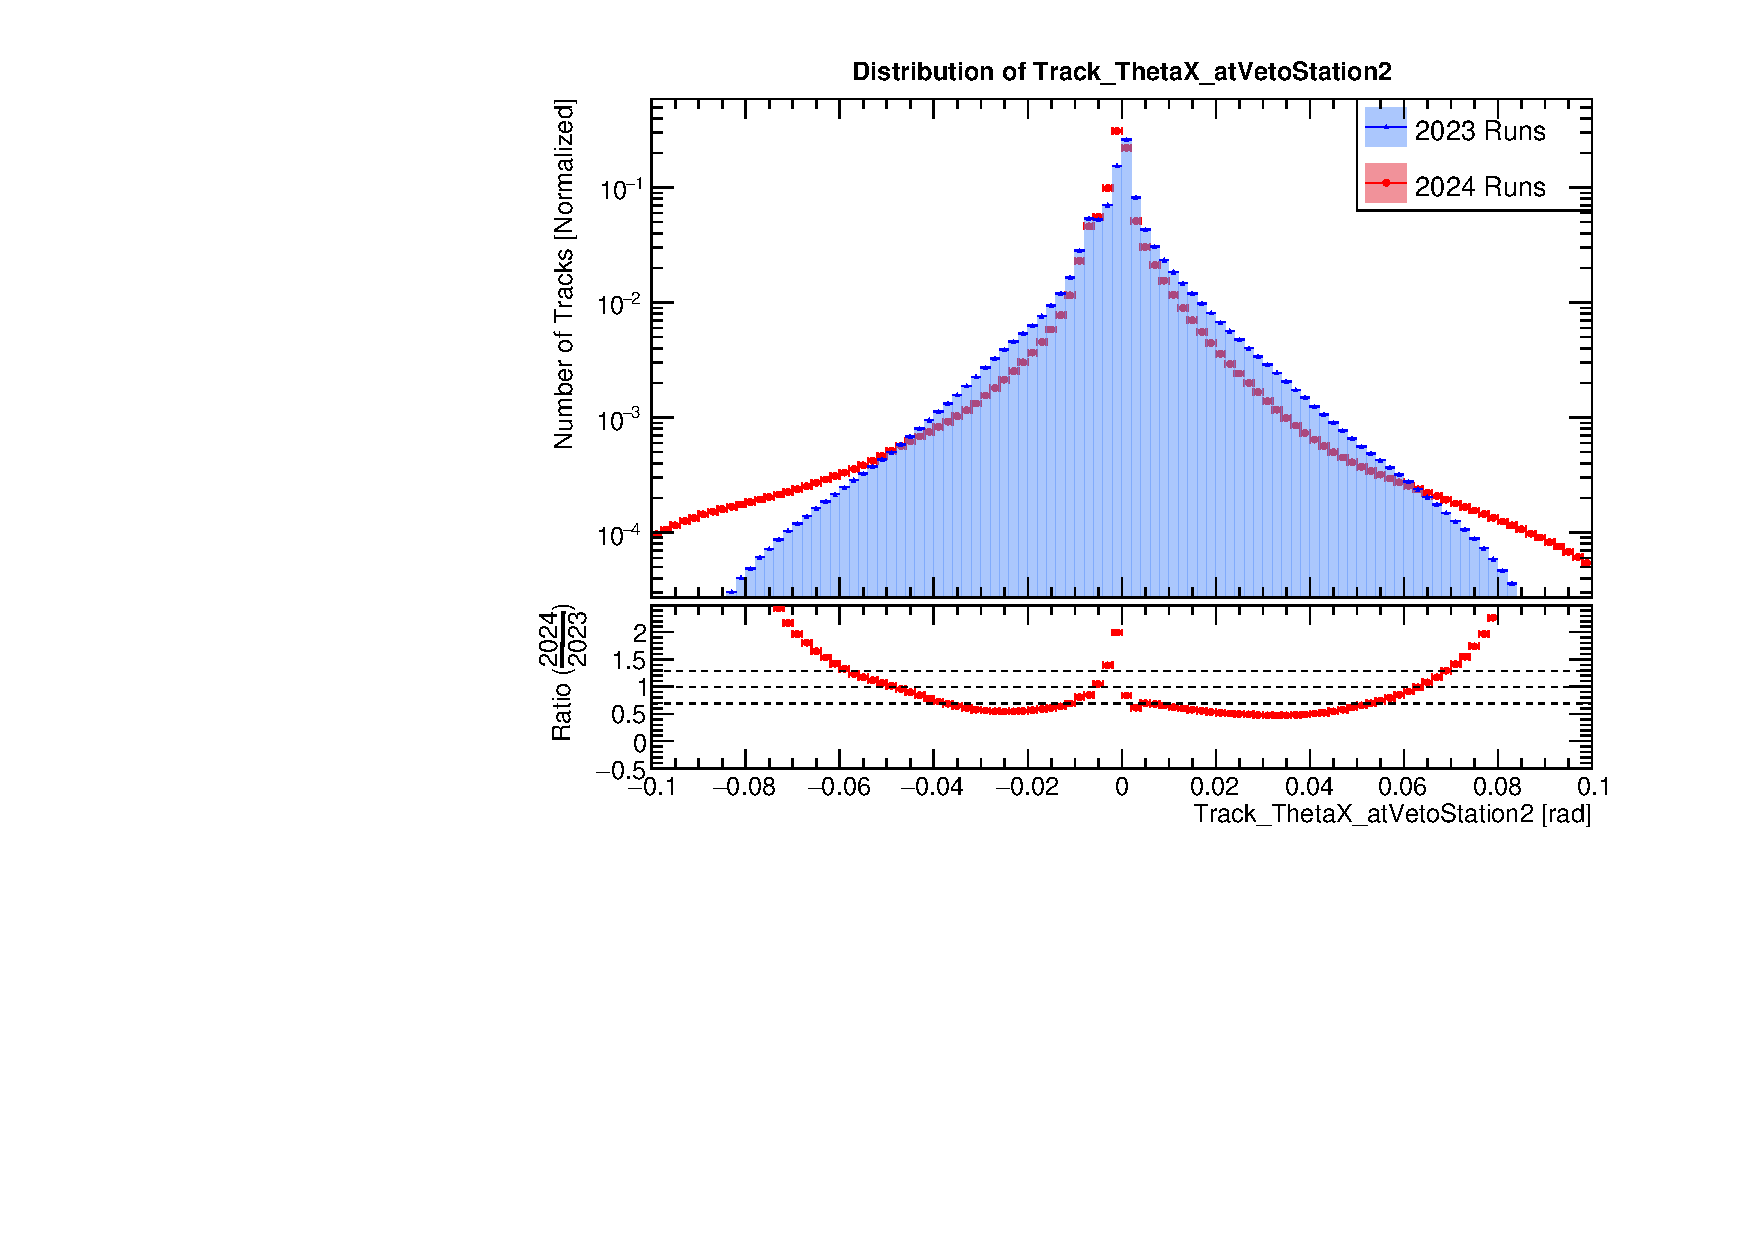
\includegraphics[width=\linewidth] {\plots/Track_ThetaX_atVetoStation2.pdf}
				\caption{Track ThetaX at VetoStation 2}
			\end{figure}
		\end{column}
		\begin{column}{0.5\textwidth}
			\begin{figure}
				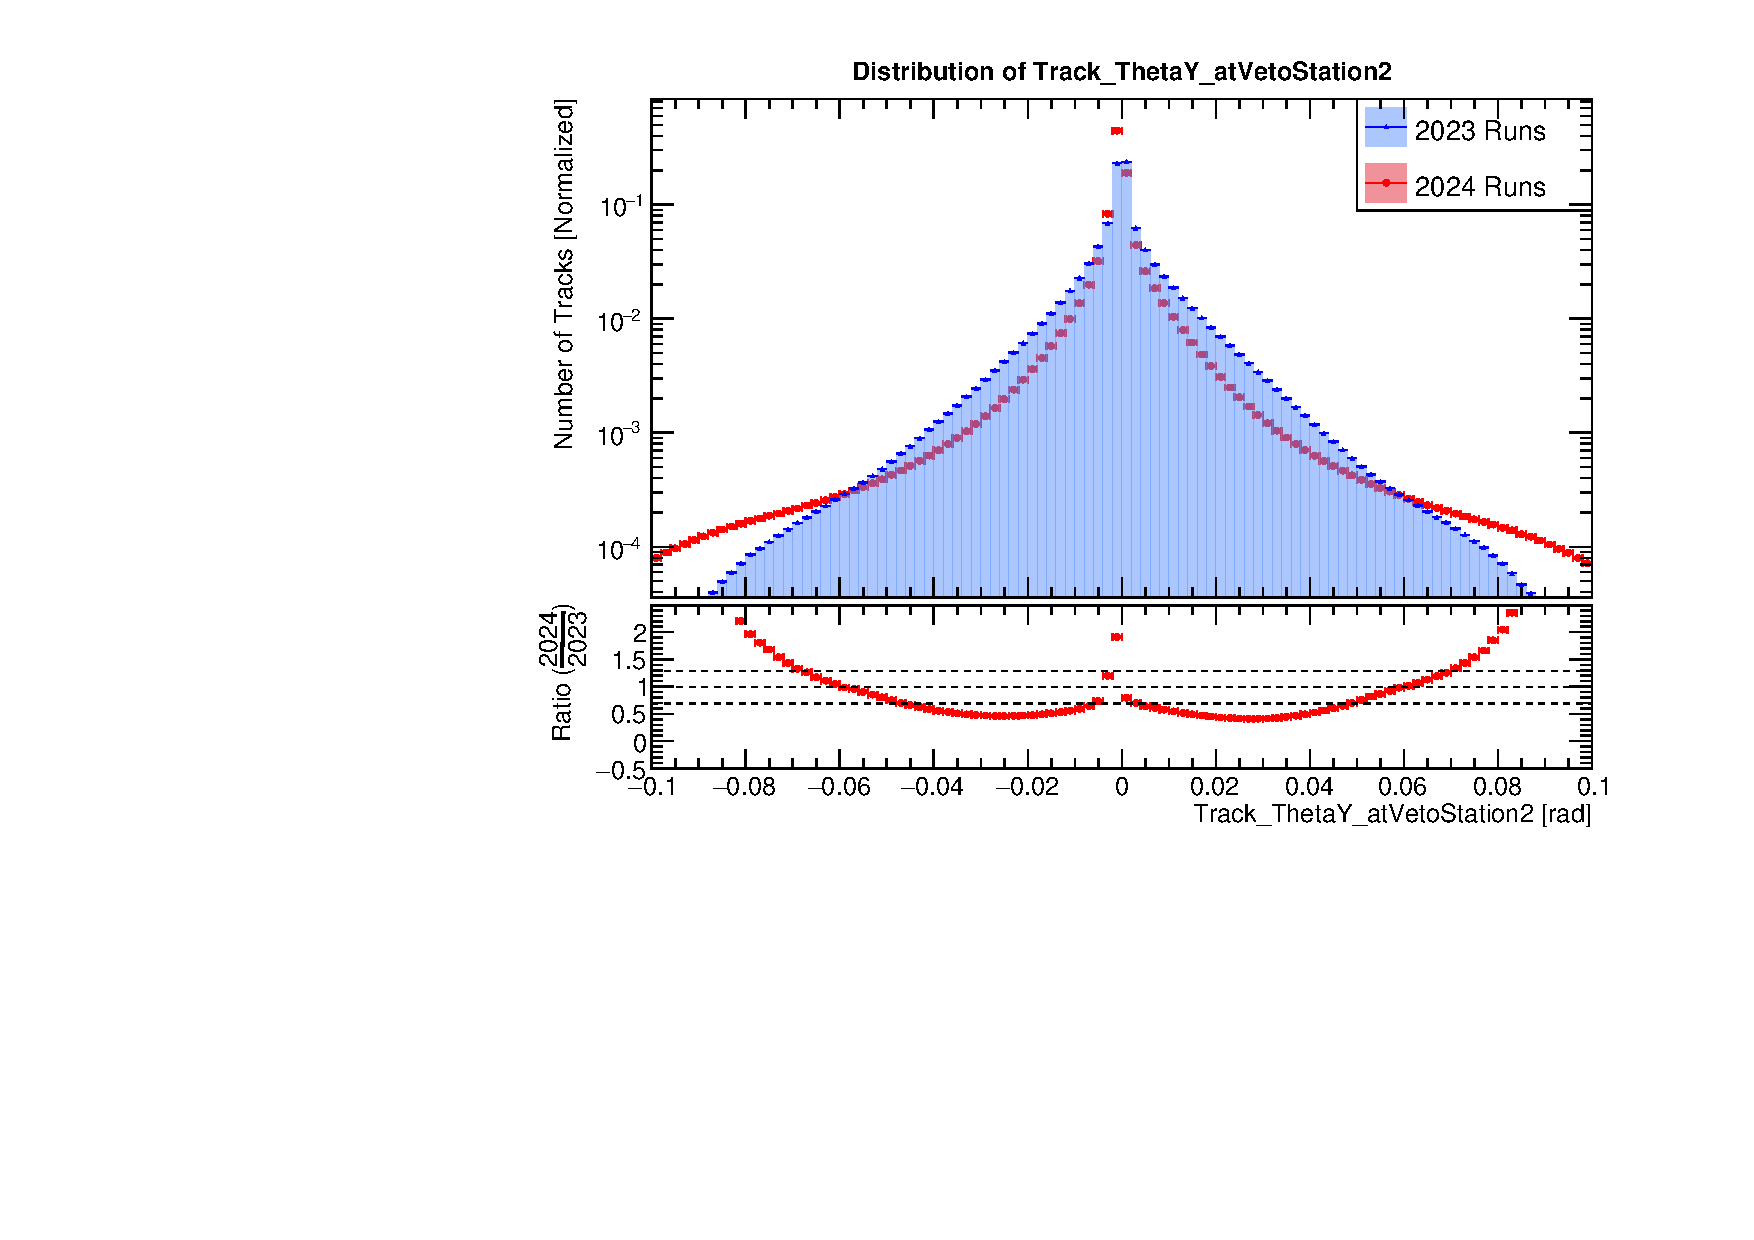
\includegraphics[width=\linewidth] {\plots/Track_ThetaY_atVetoStation2.pdf}
				\caption{Track ThetaY at VetoStation 1}
			\end{figure}
		\end{column}
	\end{columns}
\end{subframe}

\begin{subframe}{Track Angles at Trigger [SKIP]}
	\begin{columns}
		\begin{column}{0.5\textwidth}
			\begin{figure}
				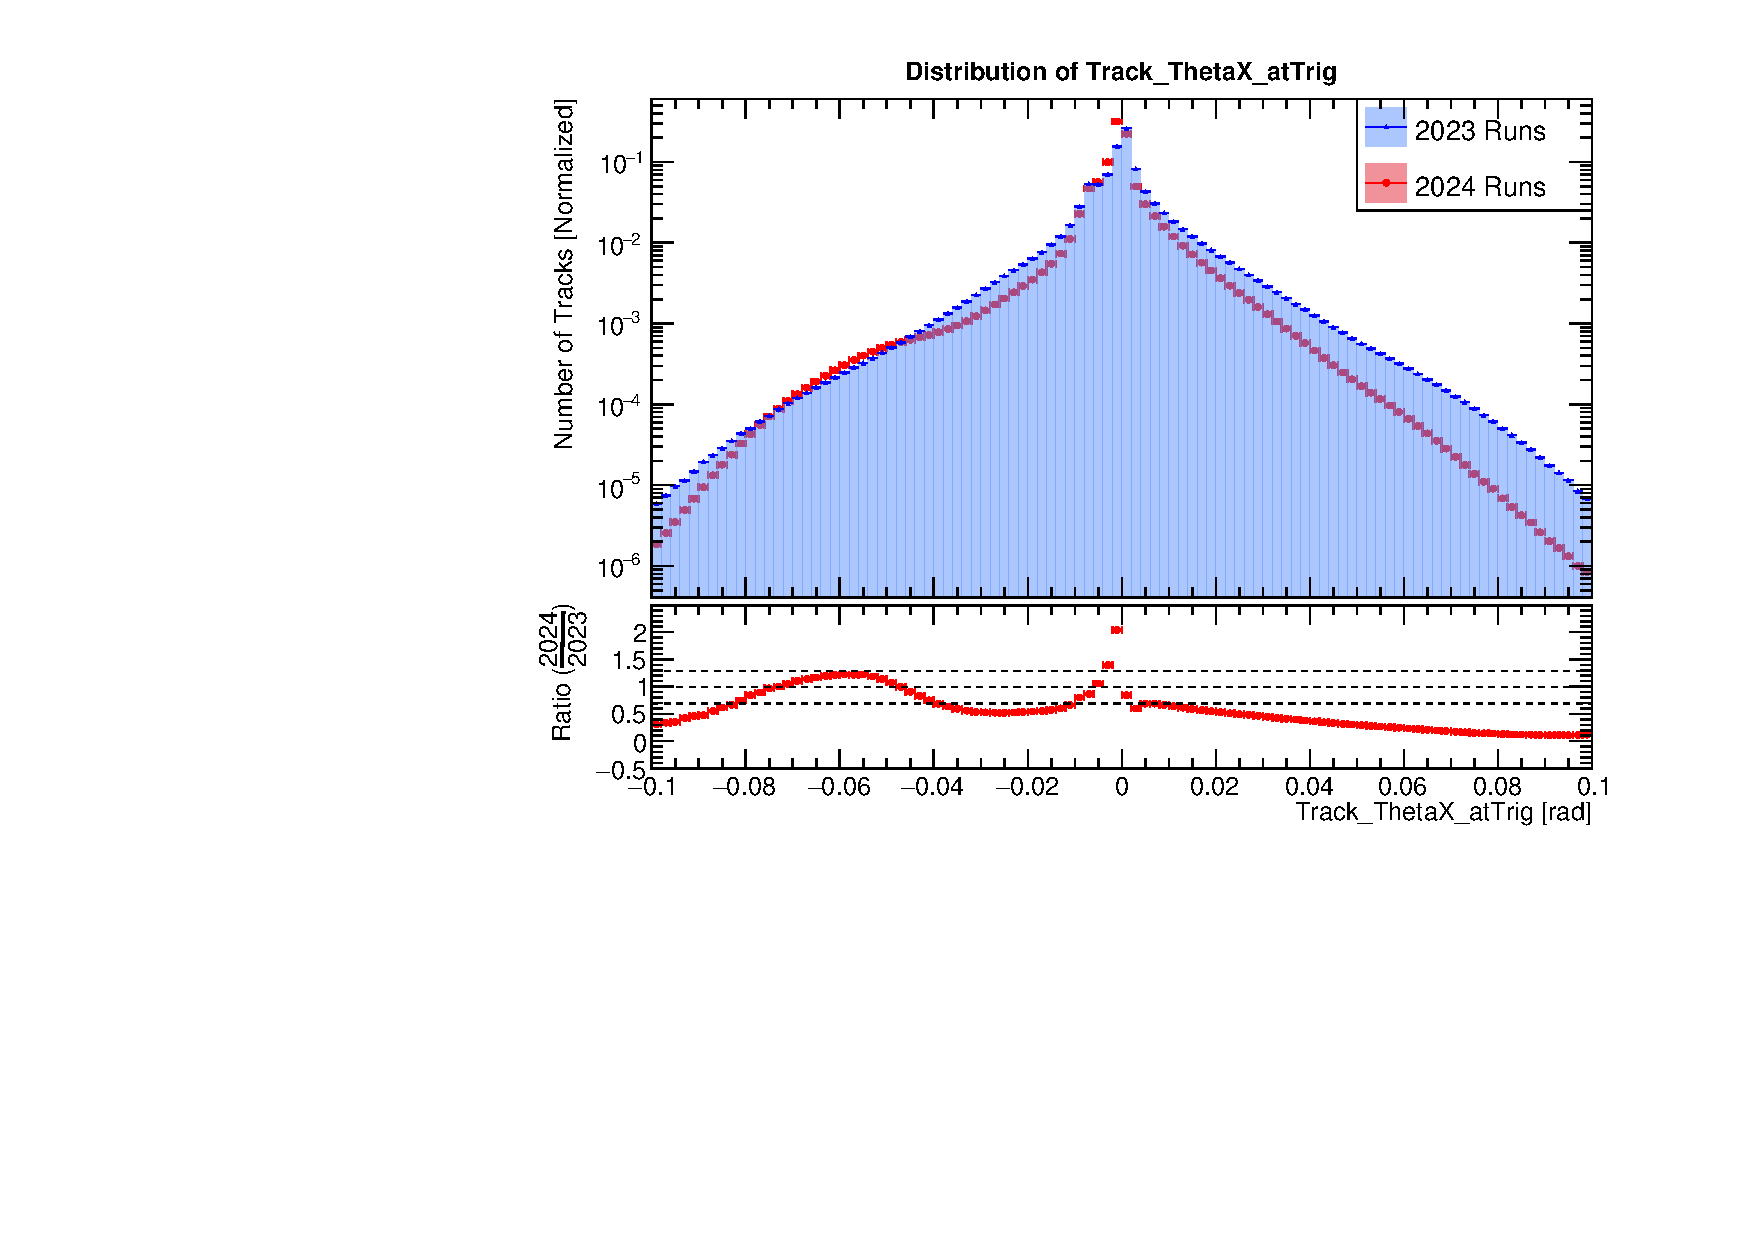
\includegraphics[width=\linewidth] {\plots/Track_ThetaX_atTrig.pdf}
				\caption{Track ThetaX at Trigger}
			\end{figure}
		\end{column}
		\begin{column}{0.5\textwidth}
			\begin{figure}
				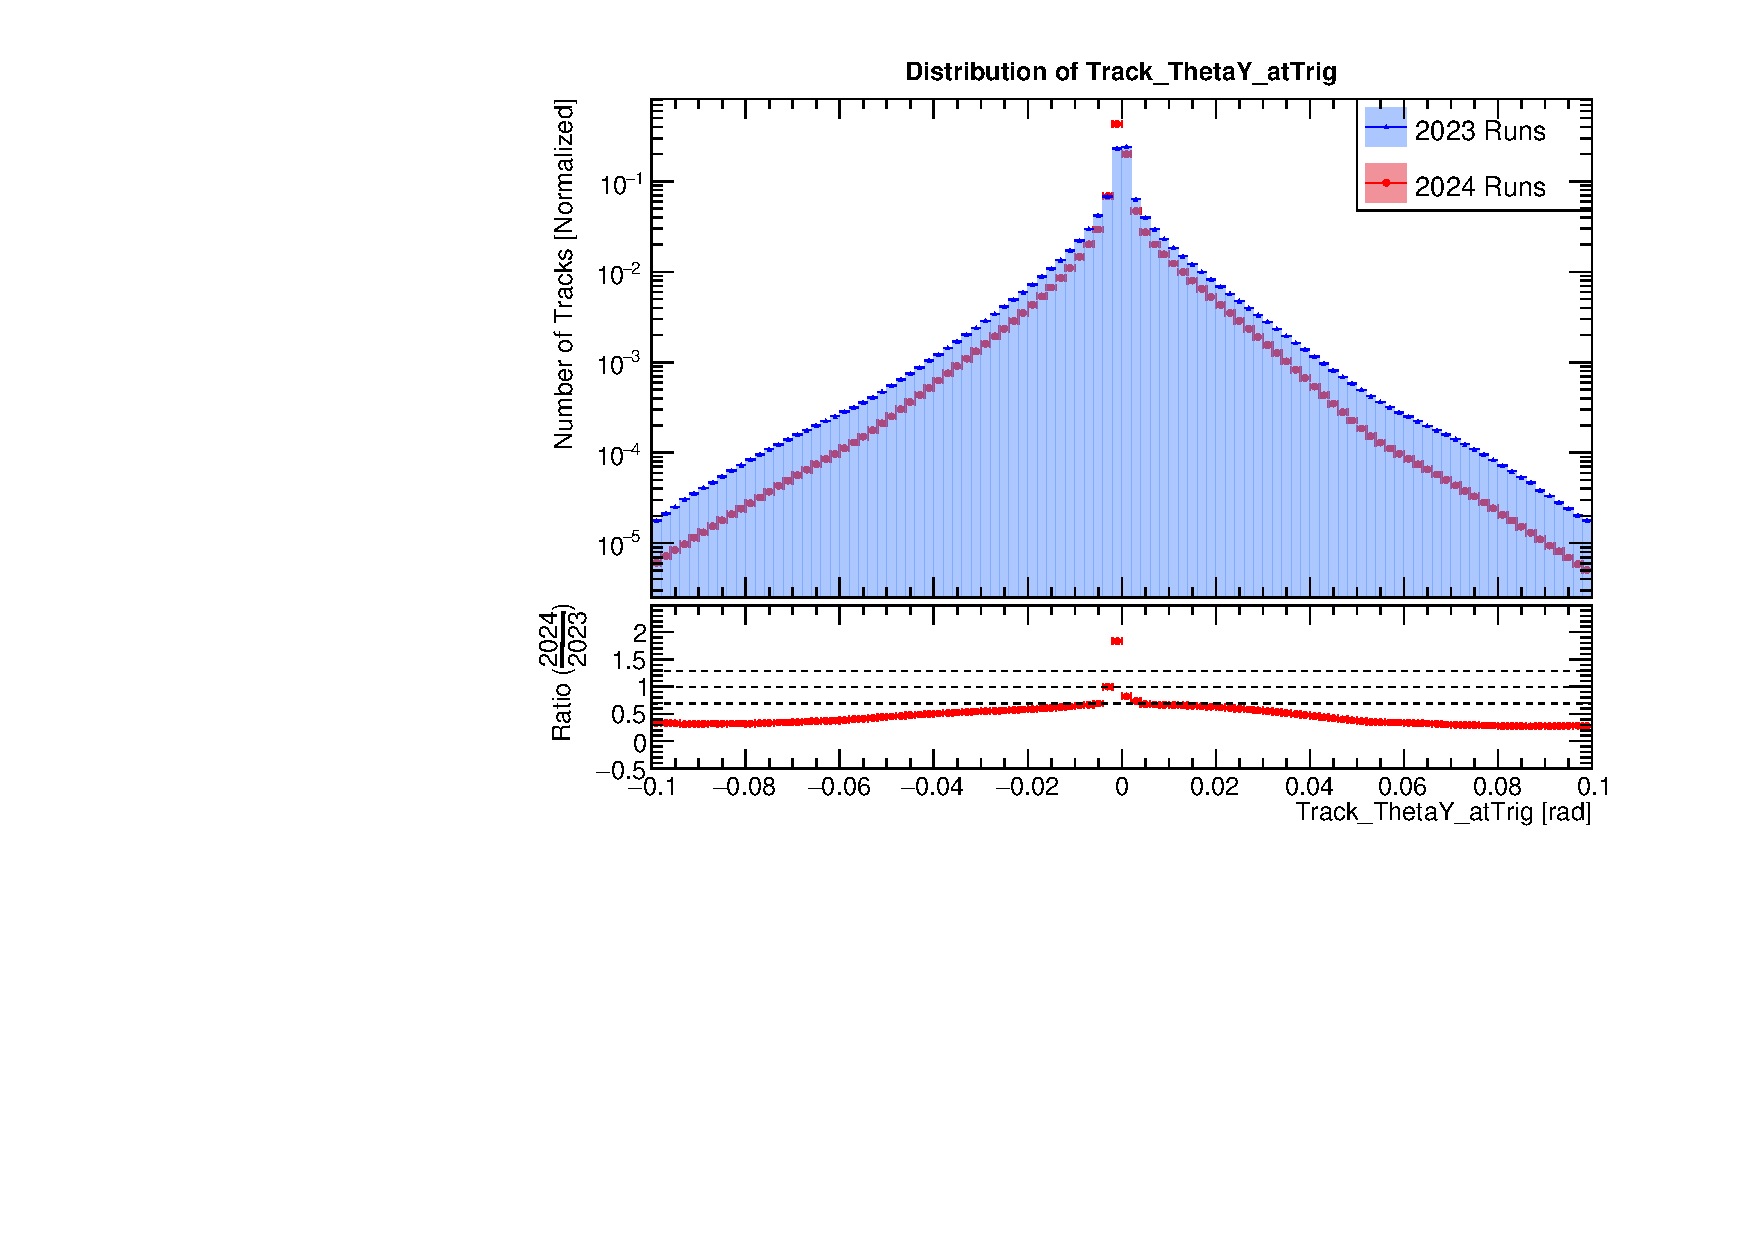
\includegraphics[width=\linewidth] {\plots/Track_ThetaY_atTrig.pdf}
				\caption{Track ThetaY at Trigger}
			\end{figure}
		\end{column}
	\end{columns}
\end{subframe}

\begin{frame}{Track Angles at Tracking Station 1}
	\begin{columns}
		\begin{column}{0.5\textwidth}
			\begin{figure}
				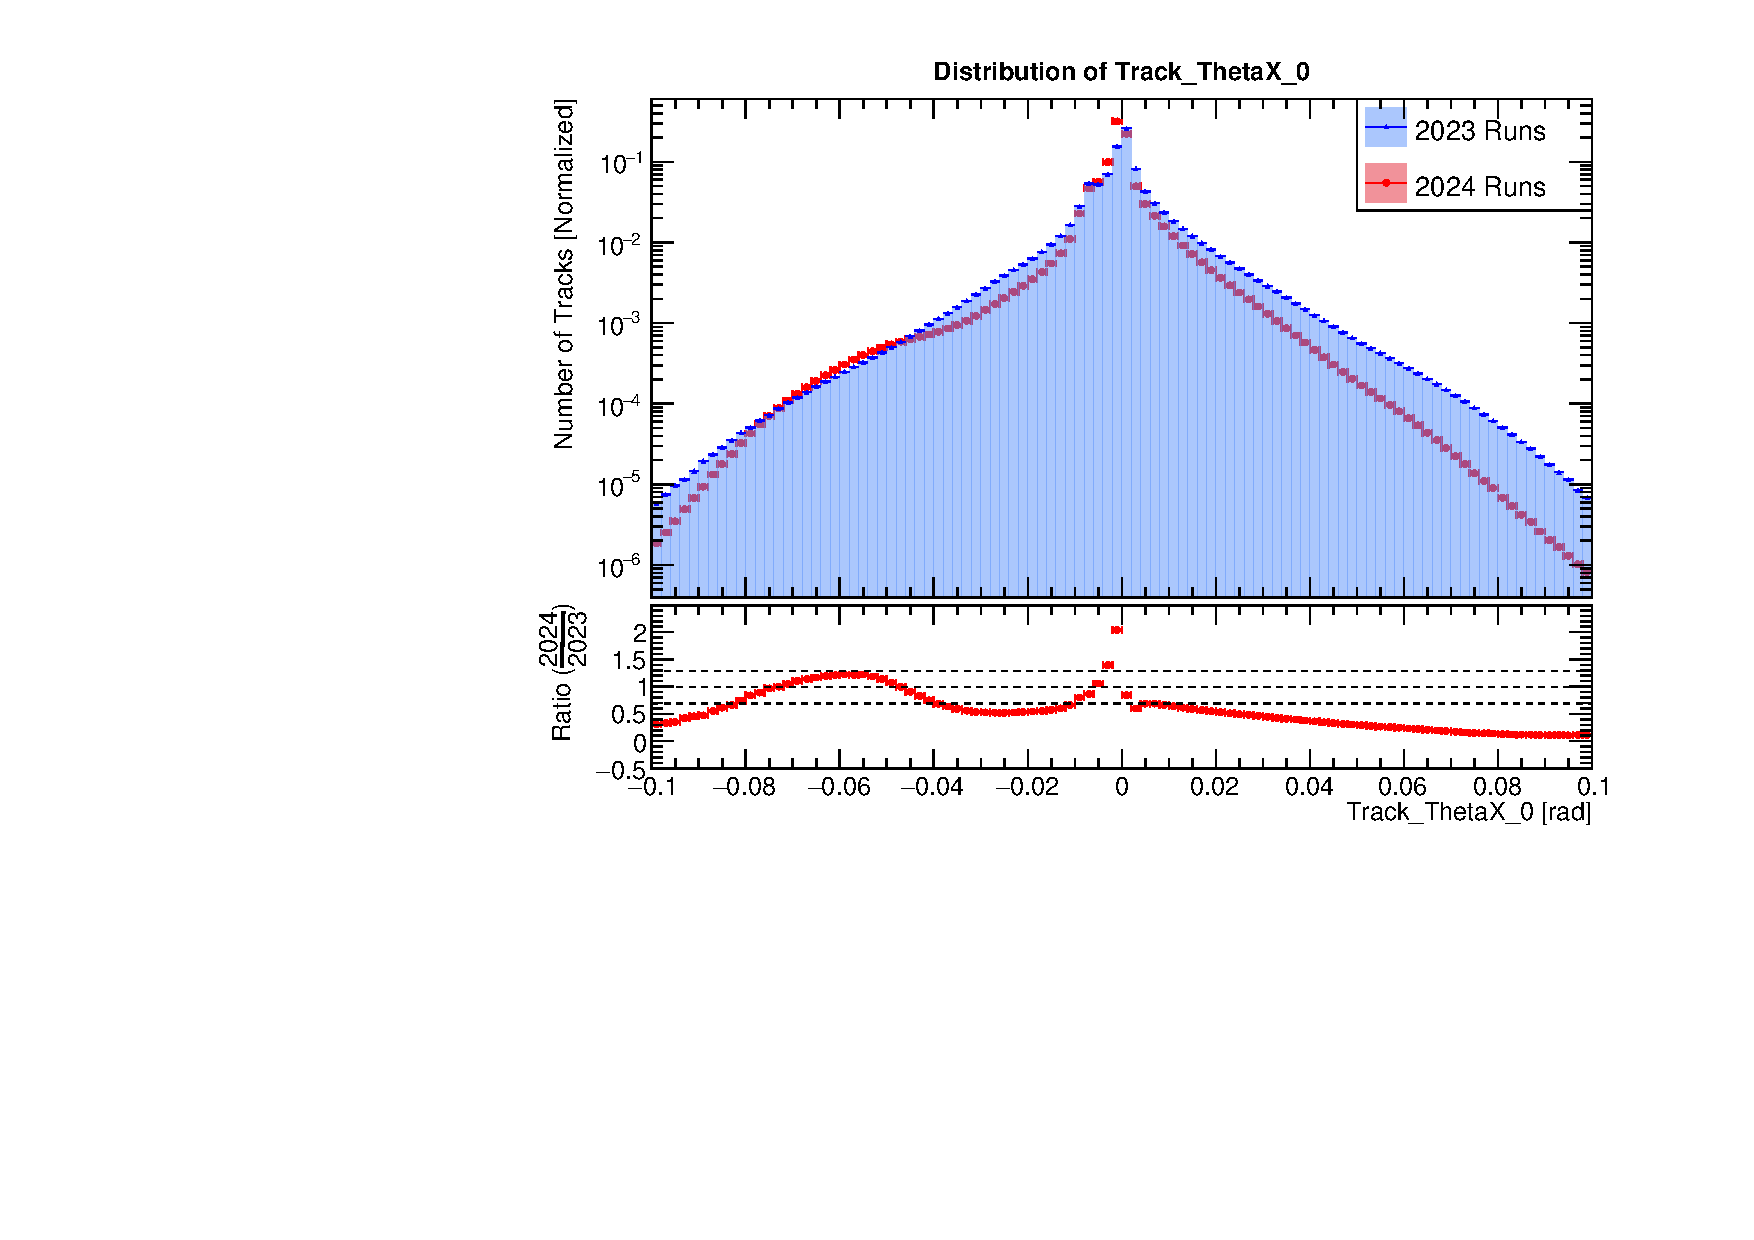
\includegraphics[width=\linewidth] {\plots/Track_ThetaX_0.pdf}
				\caption{Track ThetaX at Tracking Station 1}
			\end{figure}
		\end{column}
		\begin{column}{0.5\textwidth}
			\begin{figure}
				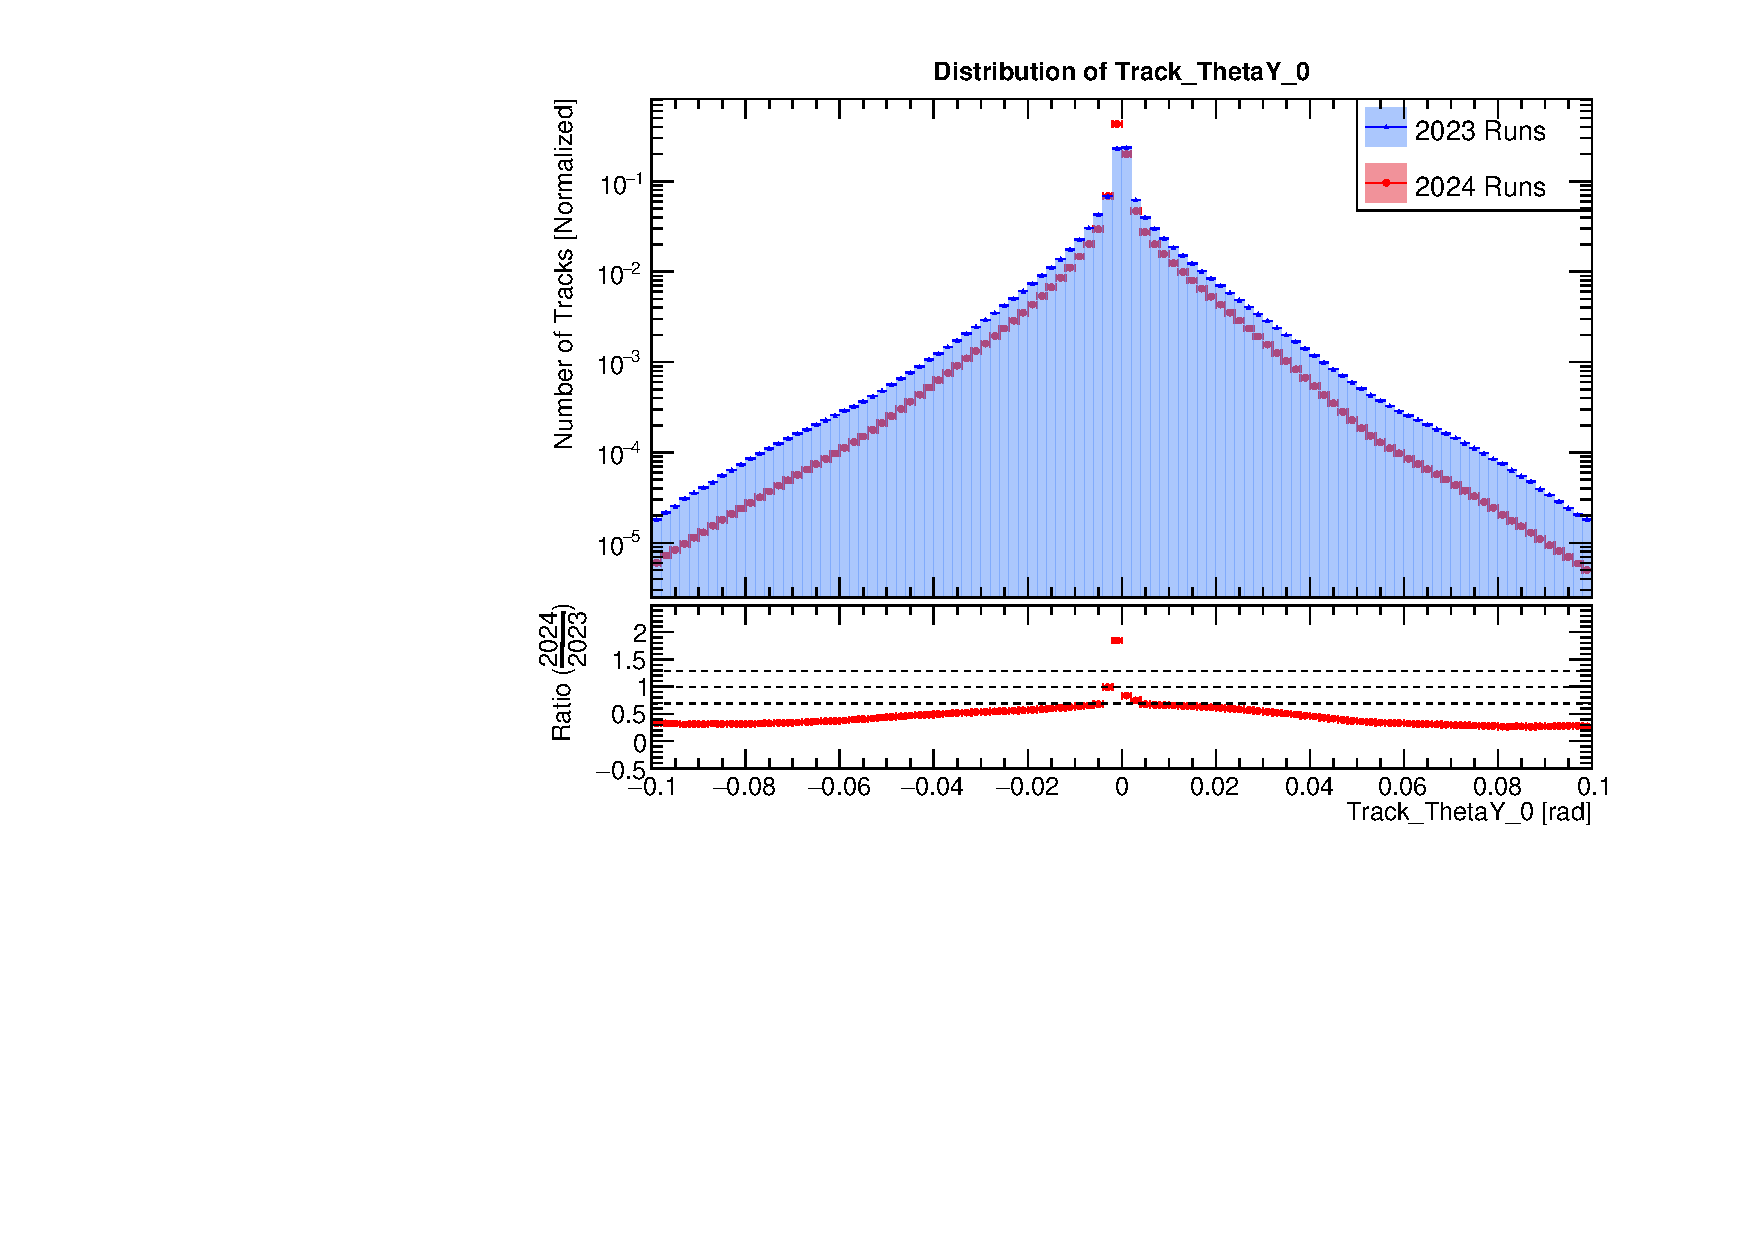
\includegraphics[width=\linewidth] {\plots/Track_ThetaY_0.pdf}
				\caption{Track ThetaY at Tracking Station 1}
			\end{figure}
		\end{column}
	\end{columns}
	\begin{itemize}
		\item There is a peak in 2024 data at -0.07 rad. Do we understand why?
		\item Similar features observed in the Background studies. [See \href{https://indico.cern.ch/event/1350790/contributions/5686387/attachments/2836819/4957405/Introduction.pdf}{Page 15-16}]
	\end{itemize}
\end{frame}

\begin{frame}{Track Angles at Tracking Station 3}
	\begin{columns}
		\begin{column}{0.5\textwidth}
			\begin{figure}
				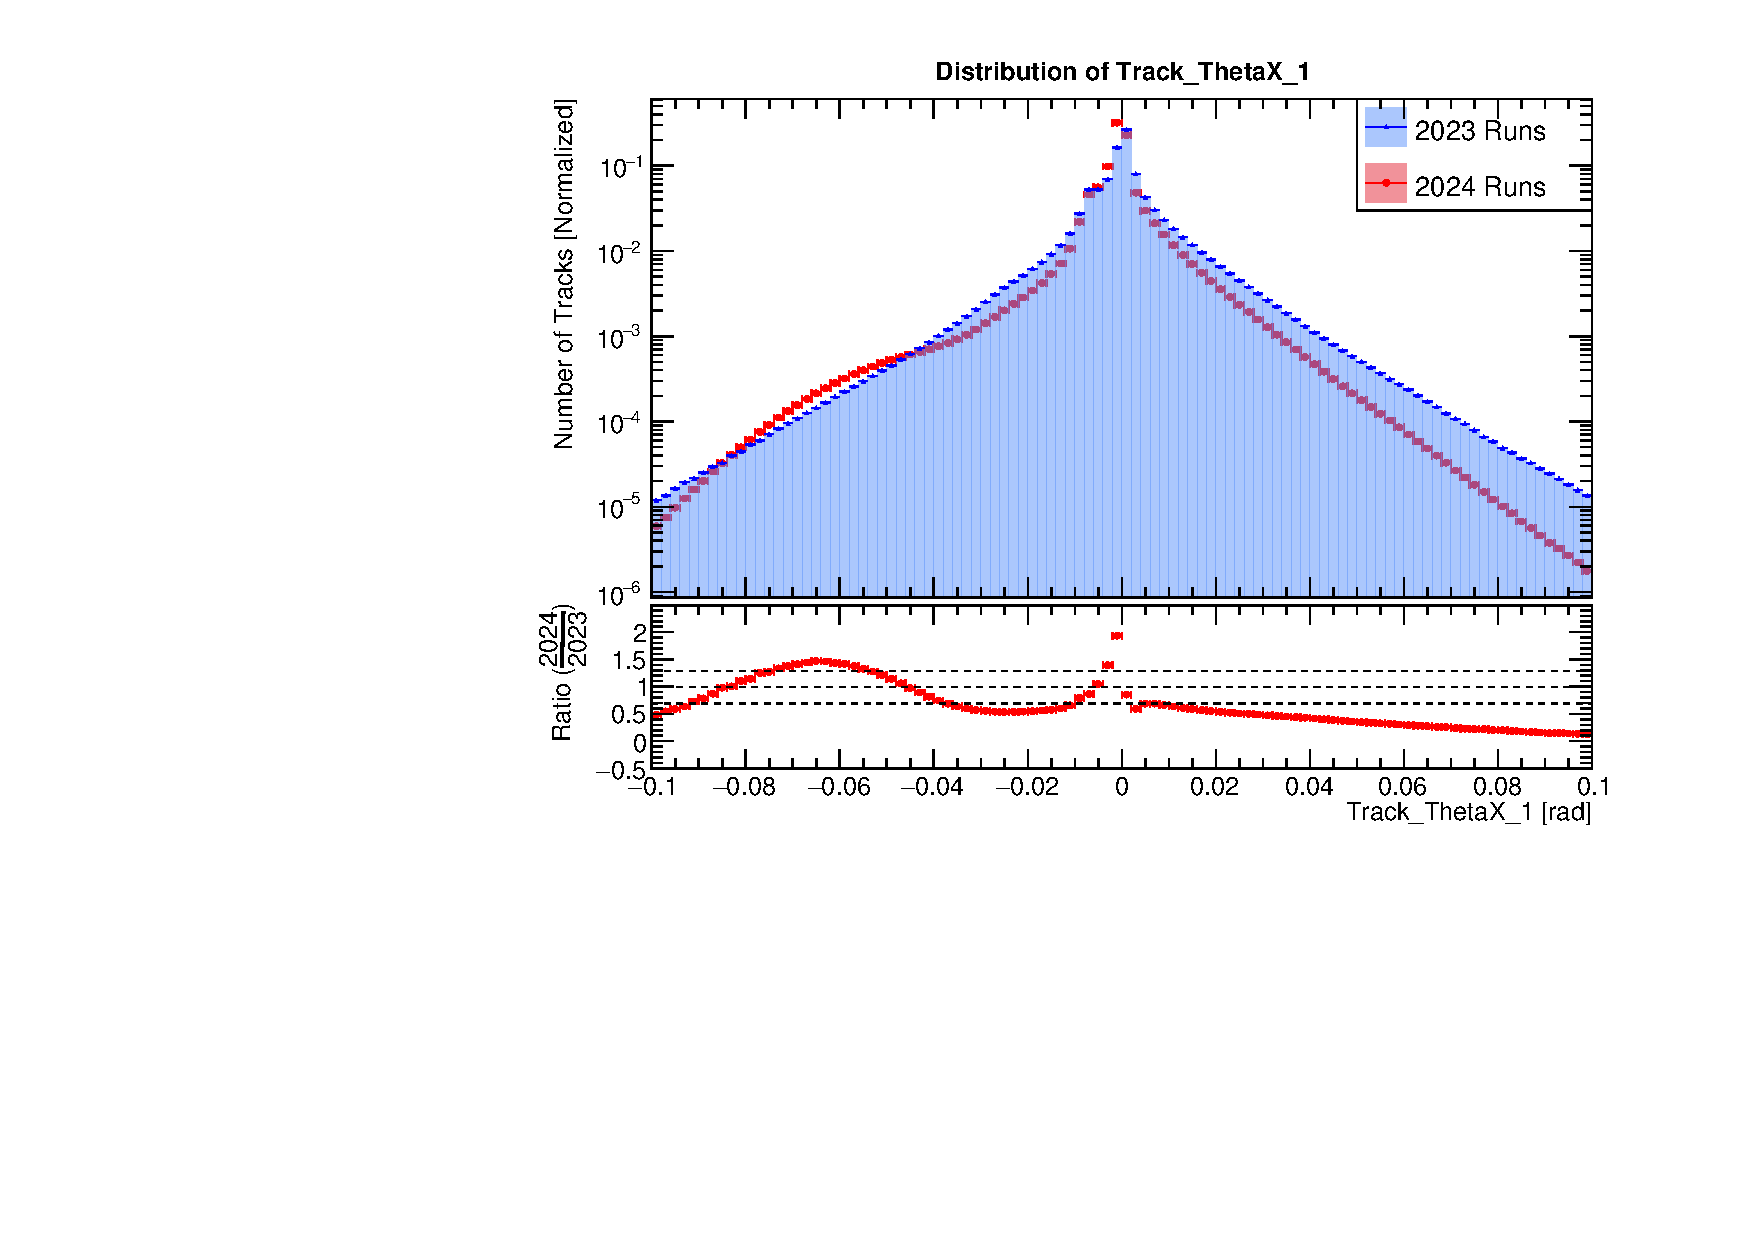
\includegraphics[width=\linewidth] {\plots/Track_ThetaX_1.pdf}
				\caption{Track ThetaX at Tracking Station 3}
			\end{figure}
		\end{column}
		\begin{column}{0.5\textwidth}
			\begin{figure}
				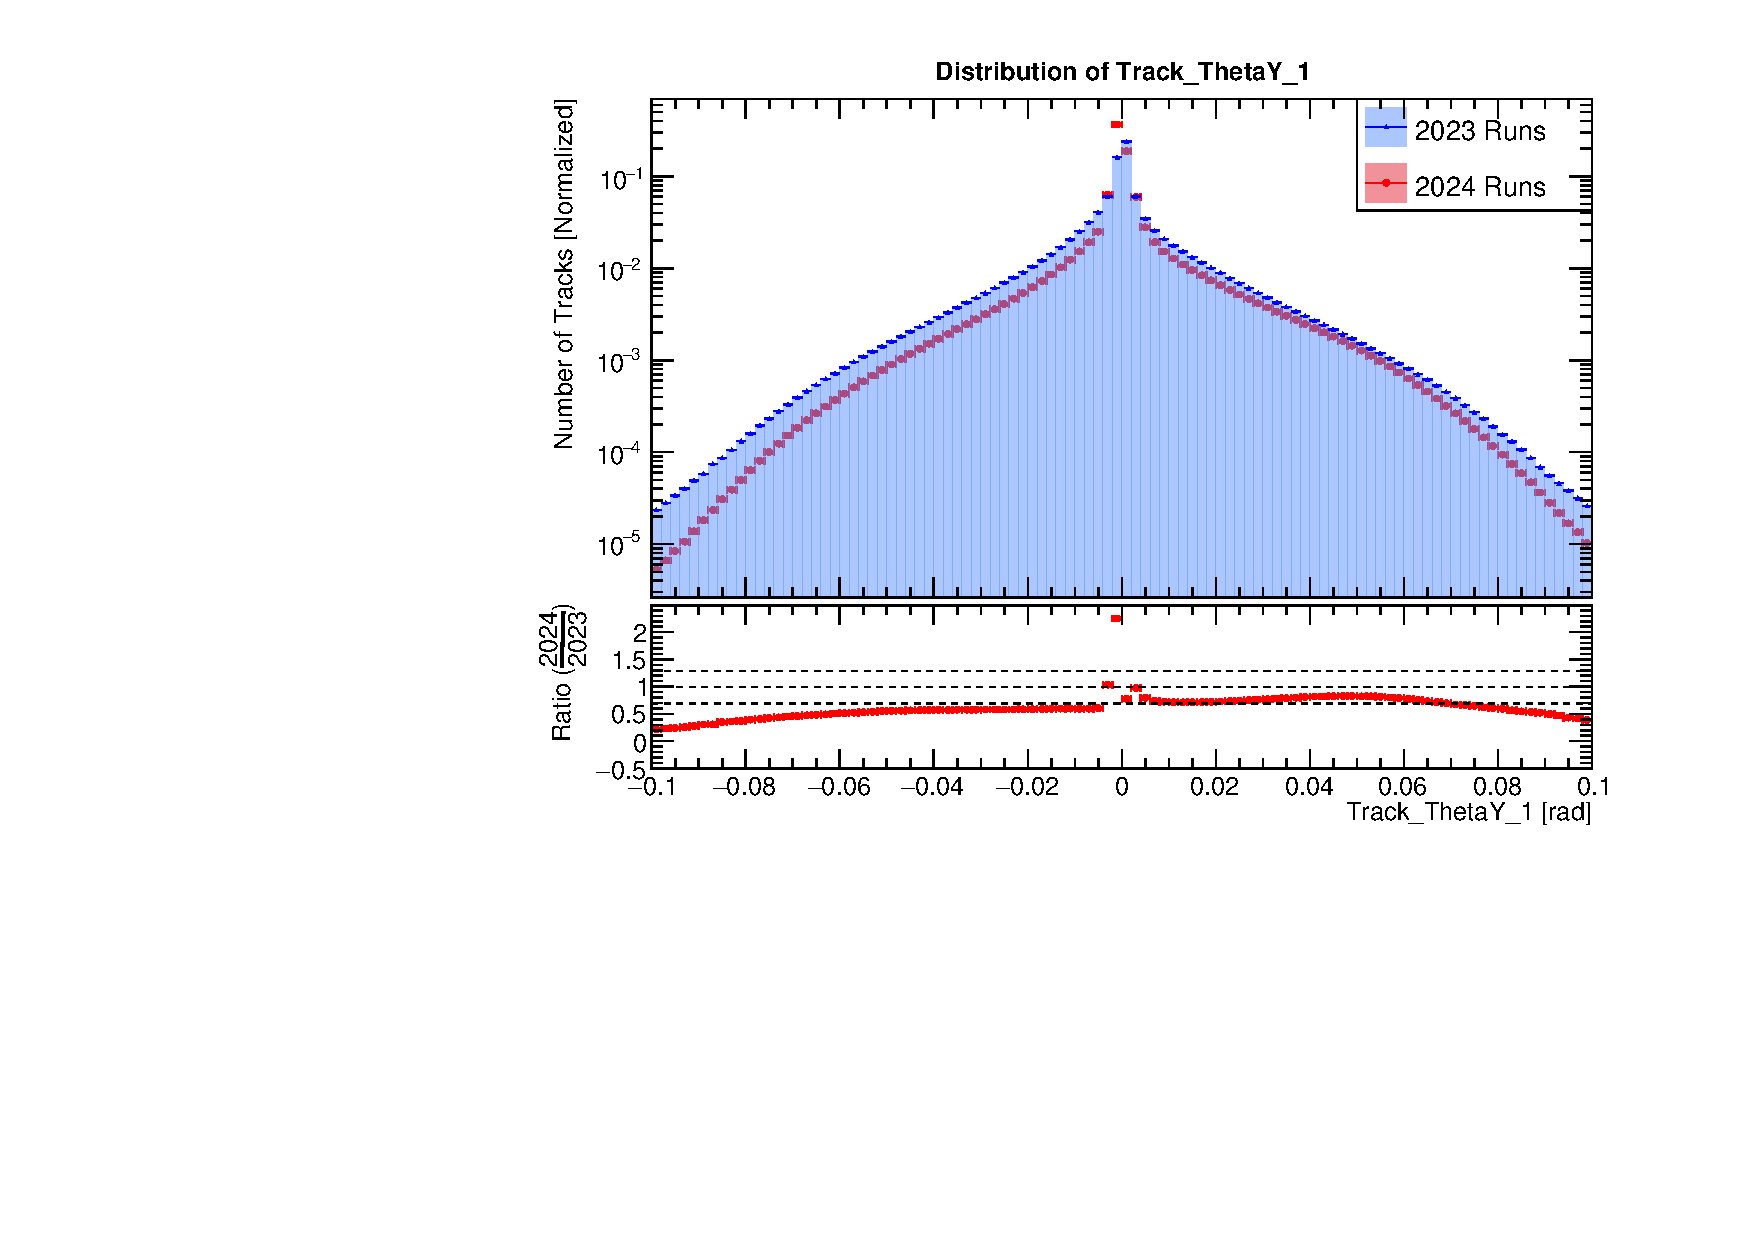
\includegraphics[width=\linewidth] {\plots/Track_ThetaY_1.pdf}
				\caption{Track ThetaX at Tracking Station 3}
			\end{figure}
		\end{column}
	\end{columns}
\end{frame}

\begin{subframe}{Track Angles at Preshower 1 [SKIP]}
	\begin{columns}
		\begin{column}{0.5\textwidth}
			\begin{figure}
				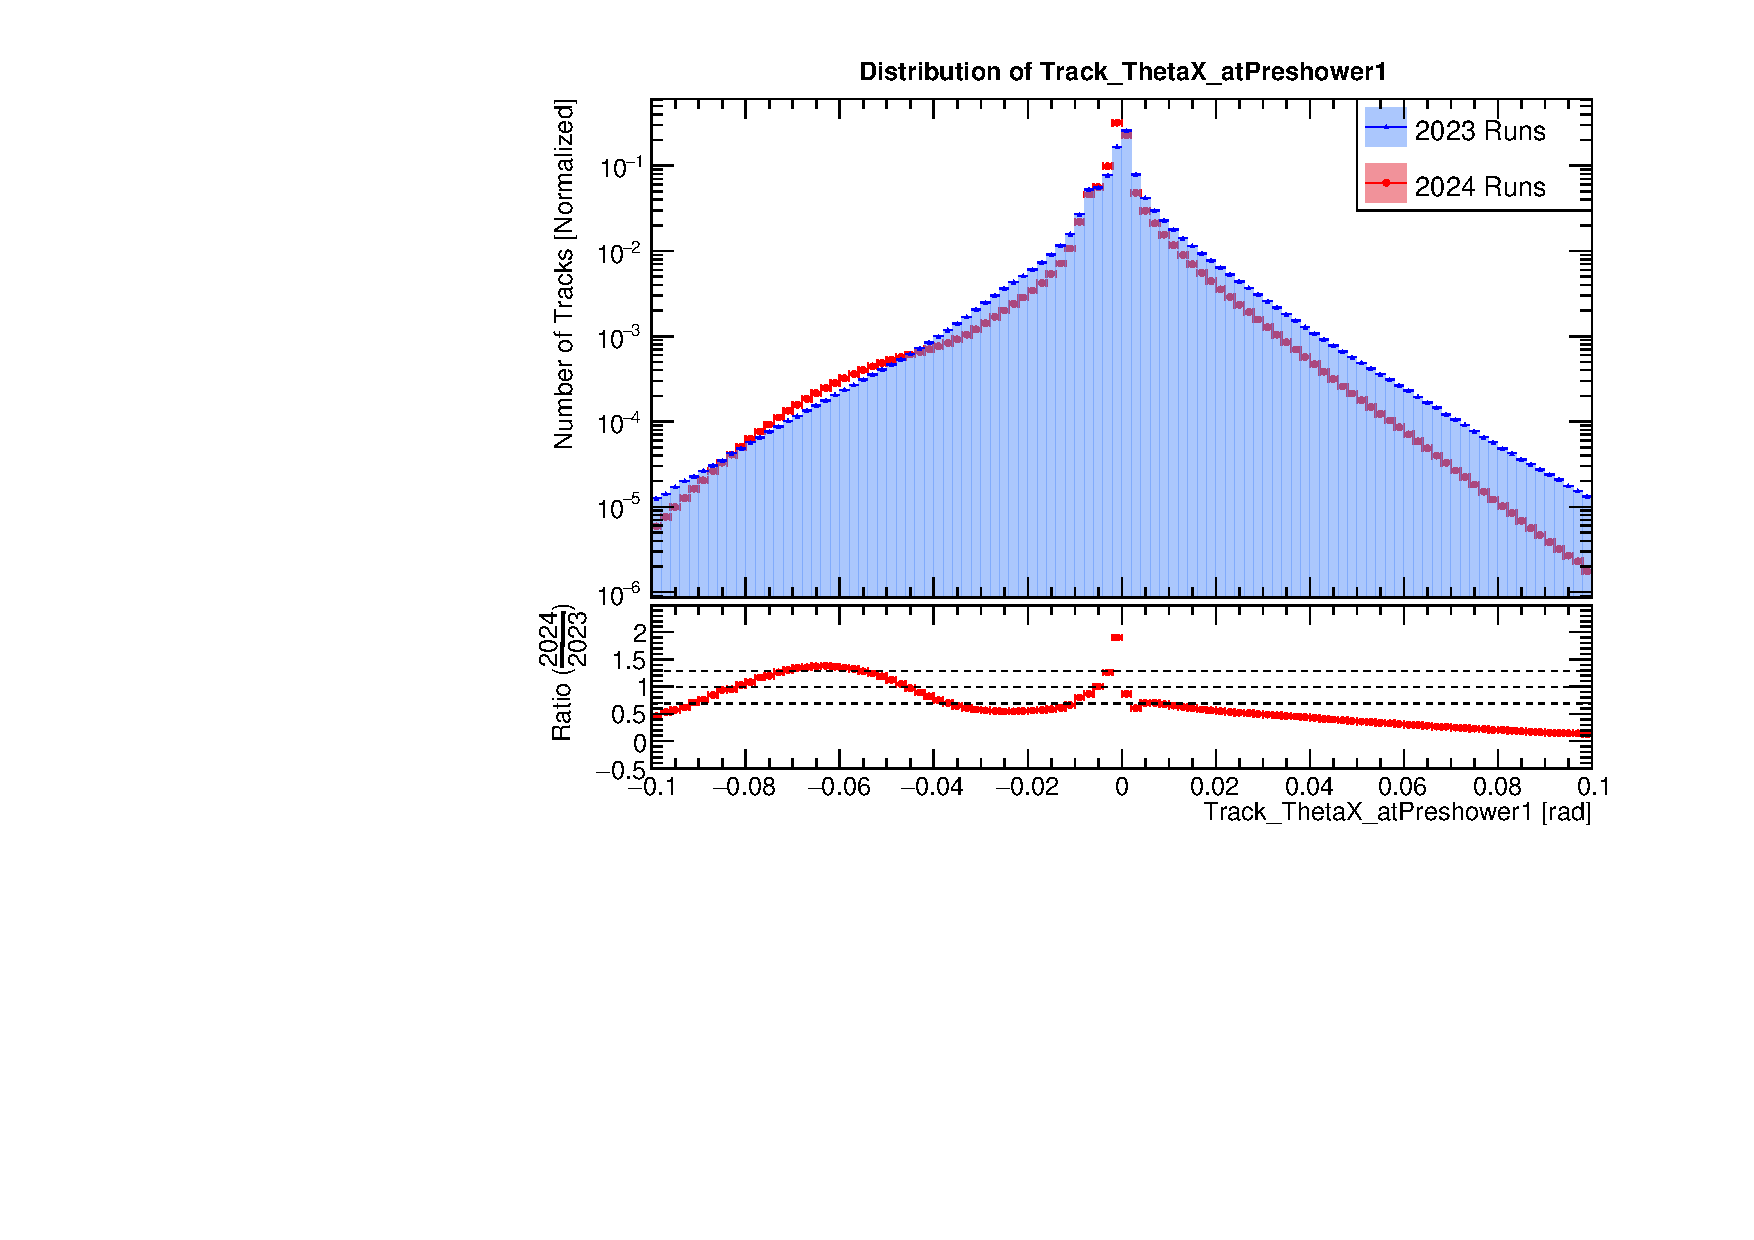
\includegraphics[width=\linewidth] {\plots/Track_ThetaX_atPreshower1.pdf}
				\caption{Track ThetaX at Preshower 1}
			\end{figure}
		\end{column}
		\begin{column}{0.5\textwidth}
			\begin{figure}
				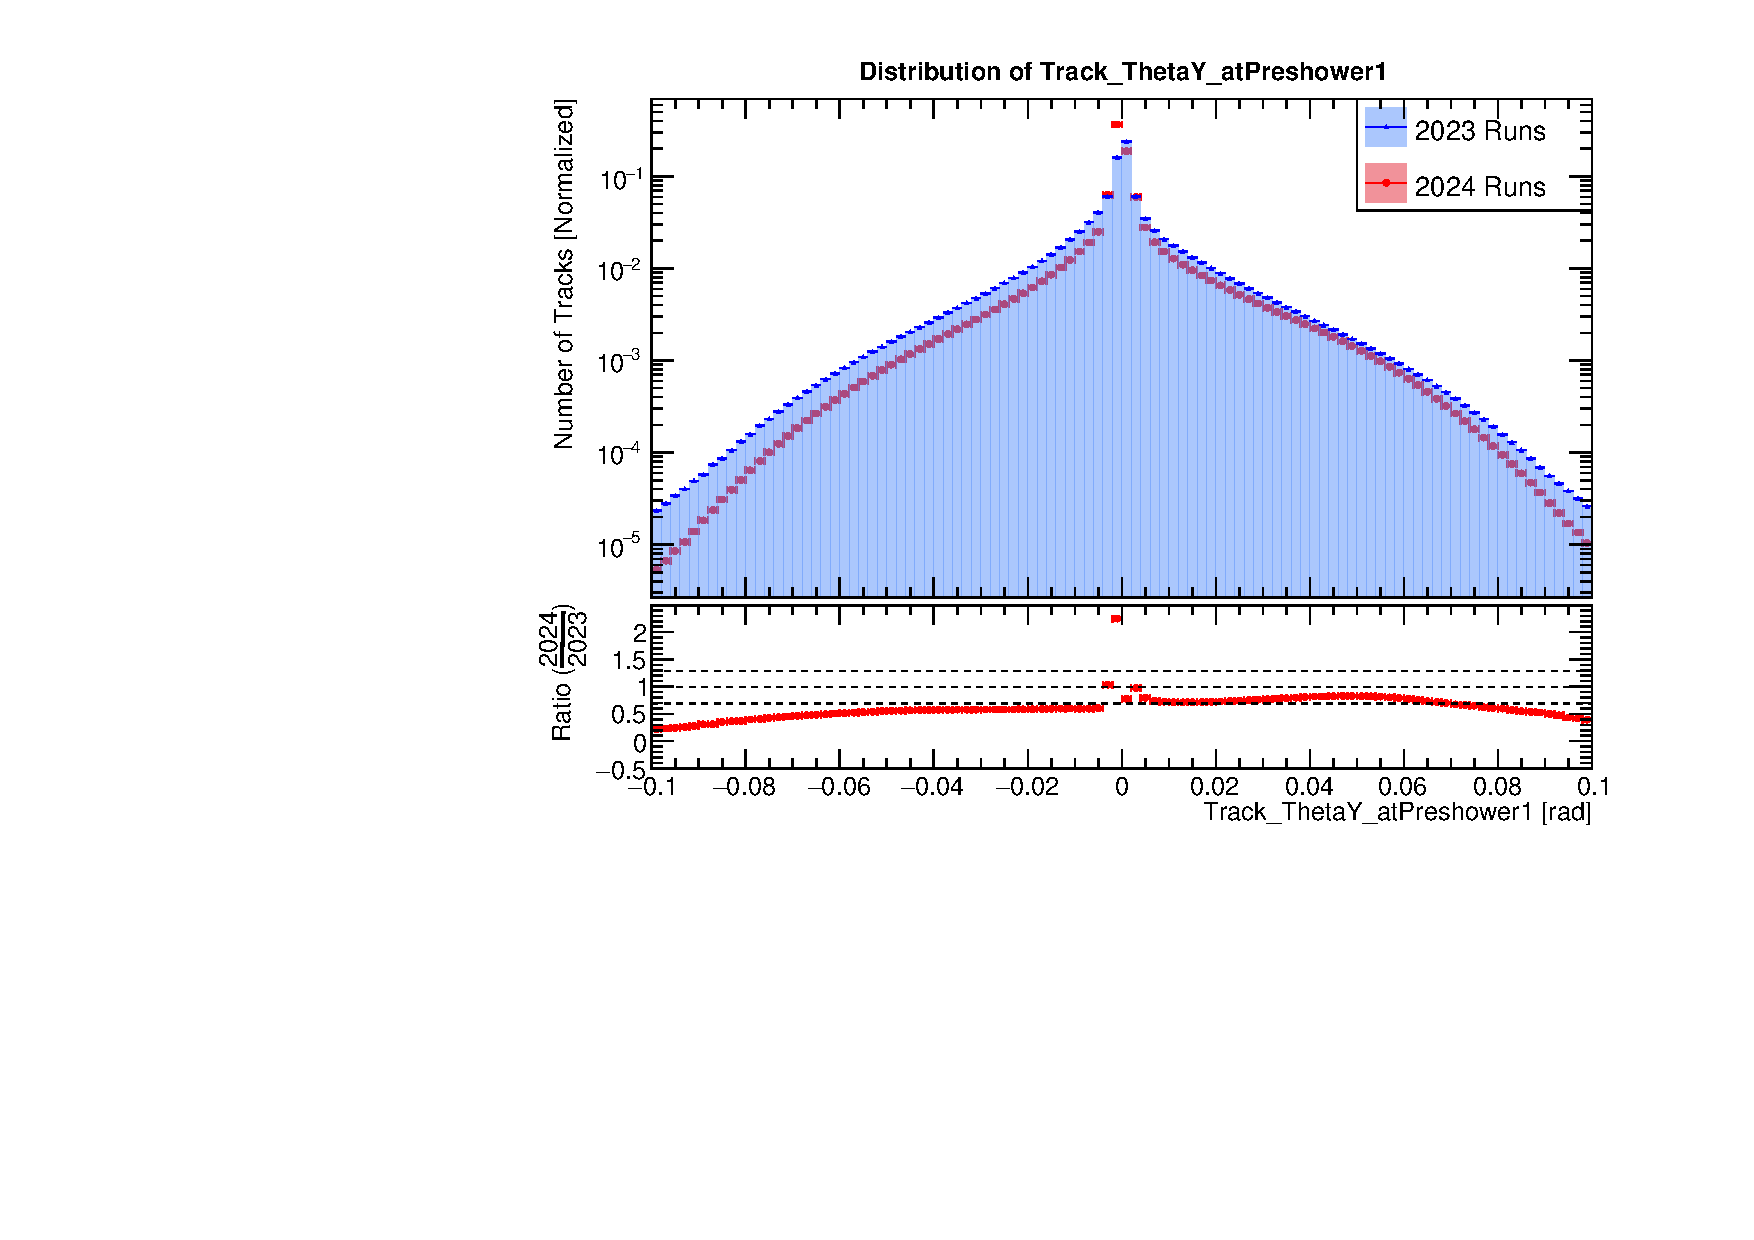
\includegraphics[width=\linewidth] {\plots/Track_ThetaY_atPreshower1.pdf}
				\caption{Track ThetaY at Preshower 1}
			\end{figure}
		\end{column}
	\end{columns}
\end{subframe}

\begin{subframe}{Track Angles at Preshower 2 [SKIP]}
	\begin{columns}
		\begin{column}{0.5\textwidth}
			\begin{figure}
				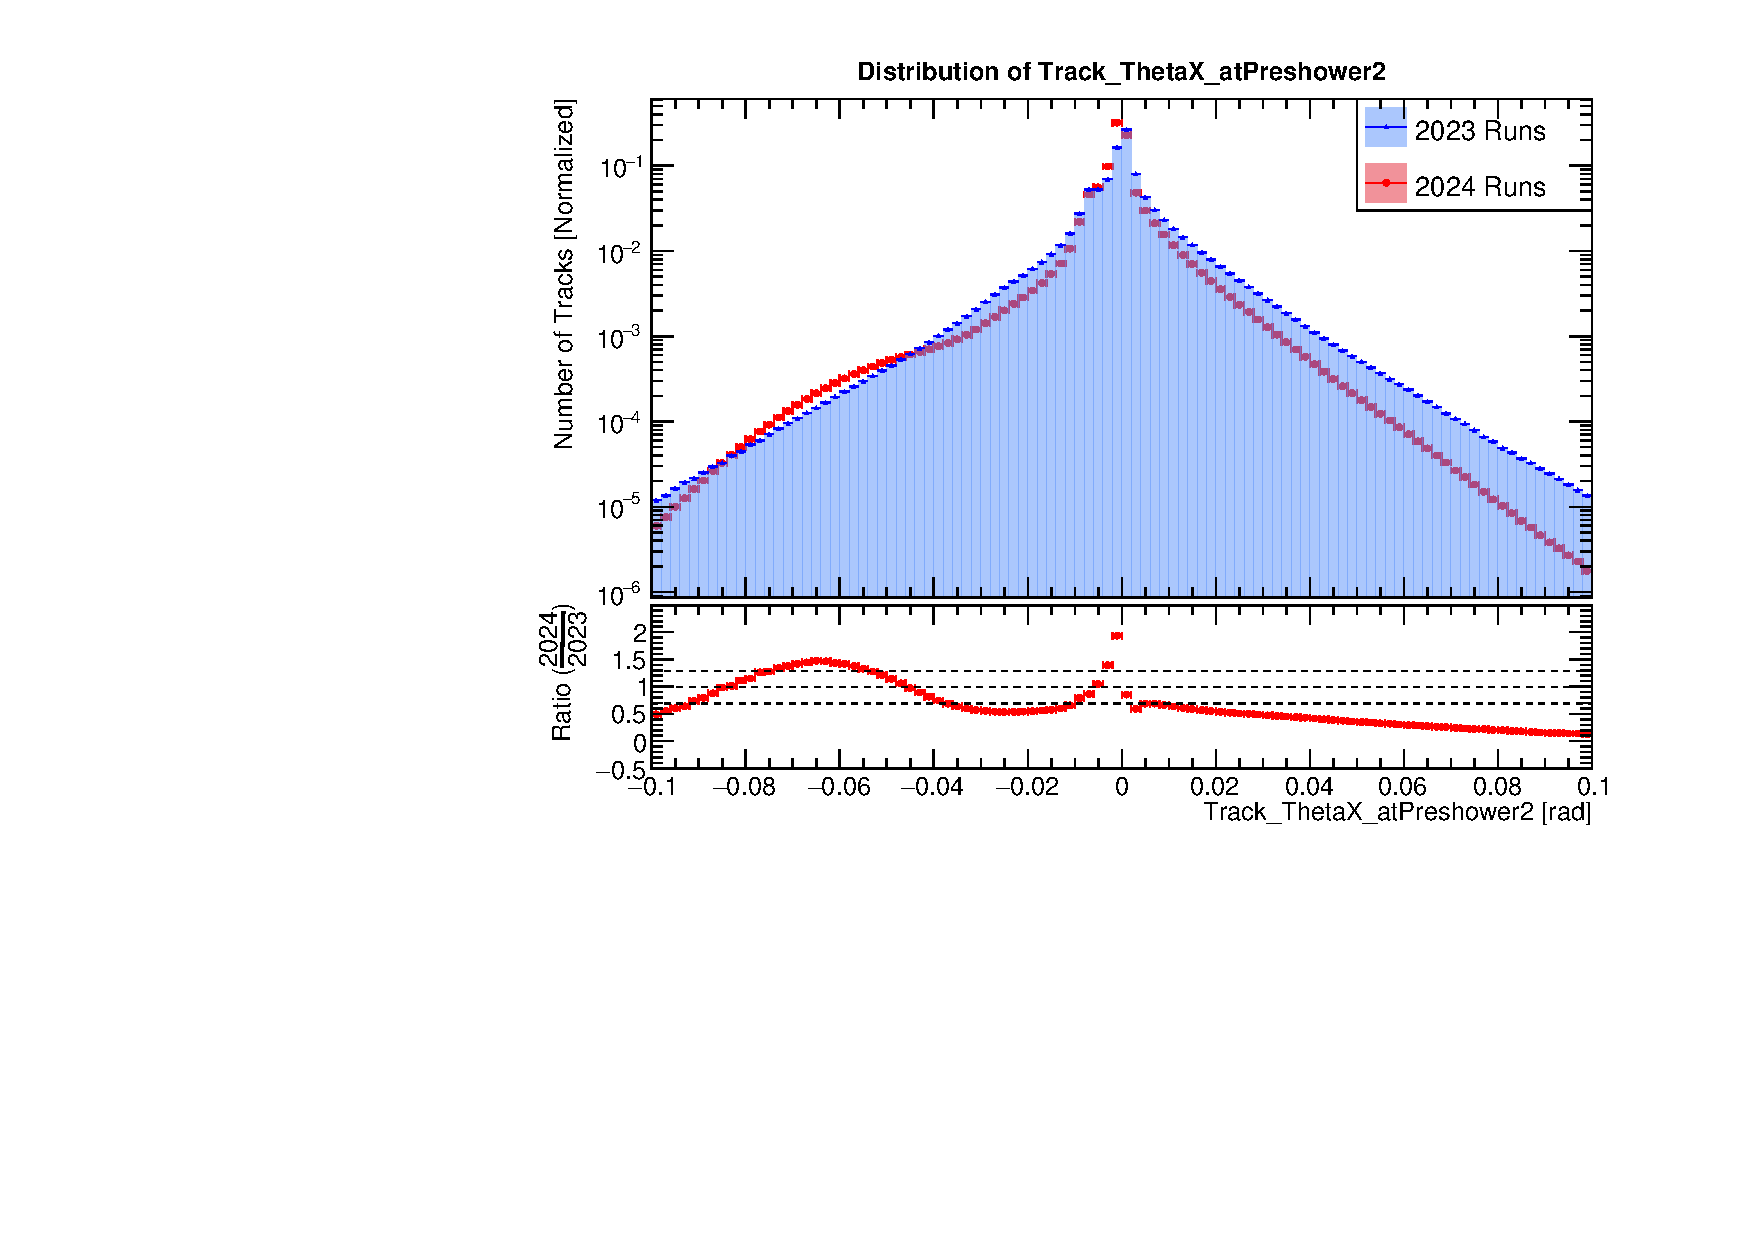
\includegraphics[width=\linewidth] {\plots/Track_ThetaX_atPreshower2.pdf}
				\caption{Track ThetaX at Preshower 2}
			\end{figure}
		\end{column}
		\begin{column}{0.5\textwidth}
			\begin{figure}
				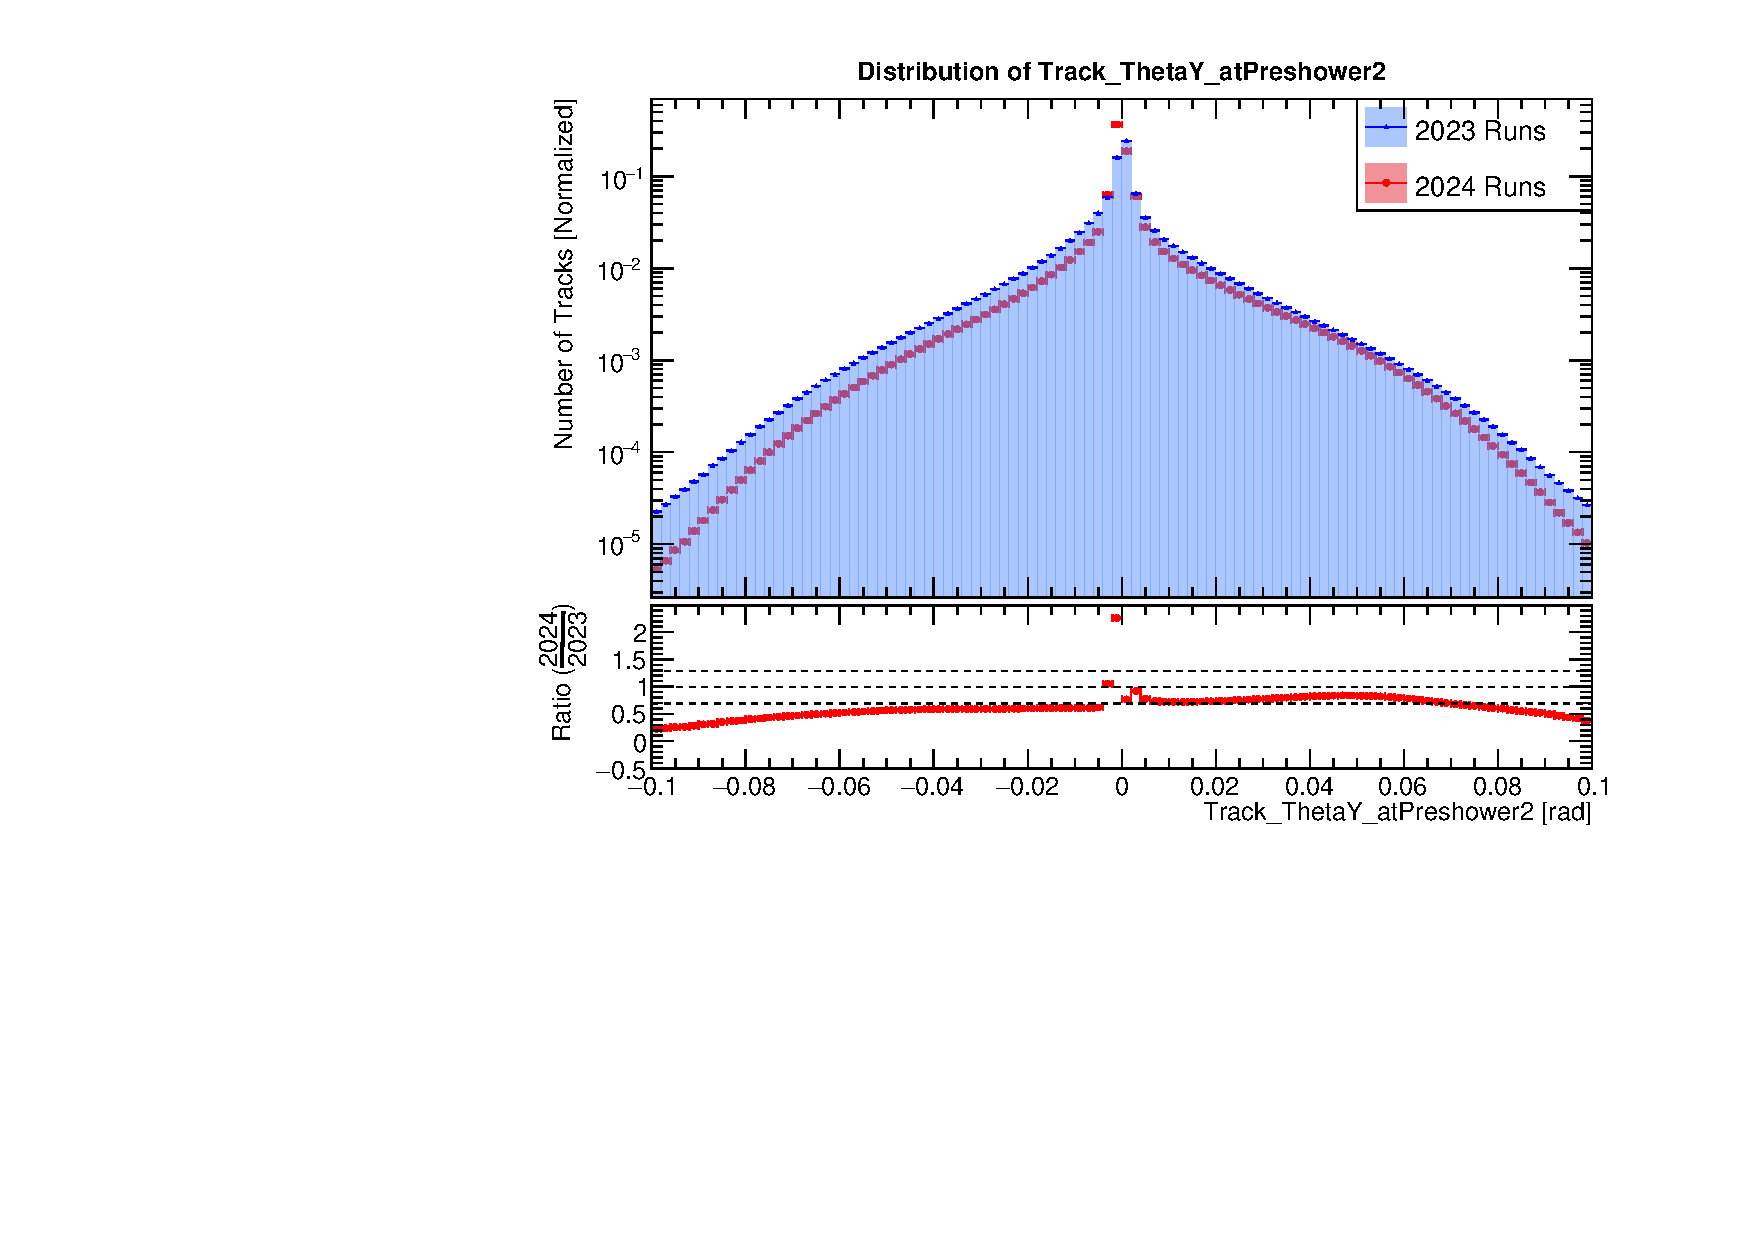
\includegraphics[width=\linewidth] {\plots/Track_ThetaY_atPreshower2.pdf}
				\caption{Track ThetaY at Preshower 2}
			\end{figure}
		\end{column}
	\end{columns}
\end{subframe}

\begin{frame}{Track Angles at Calo}
	\begin{columns}
		\begin{column}{0.5\textwidth}
			\begin{figure}
				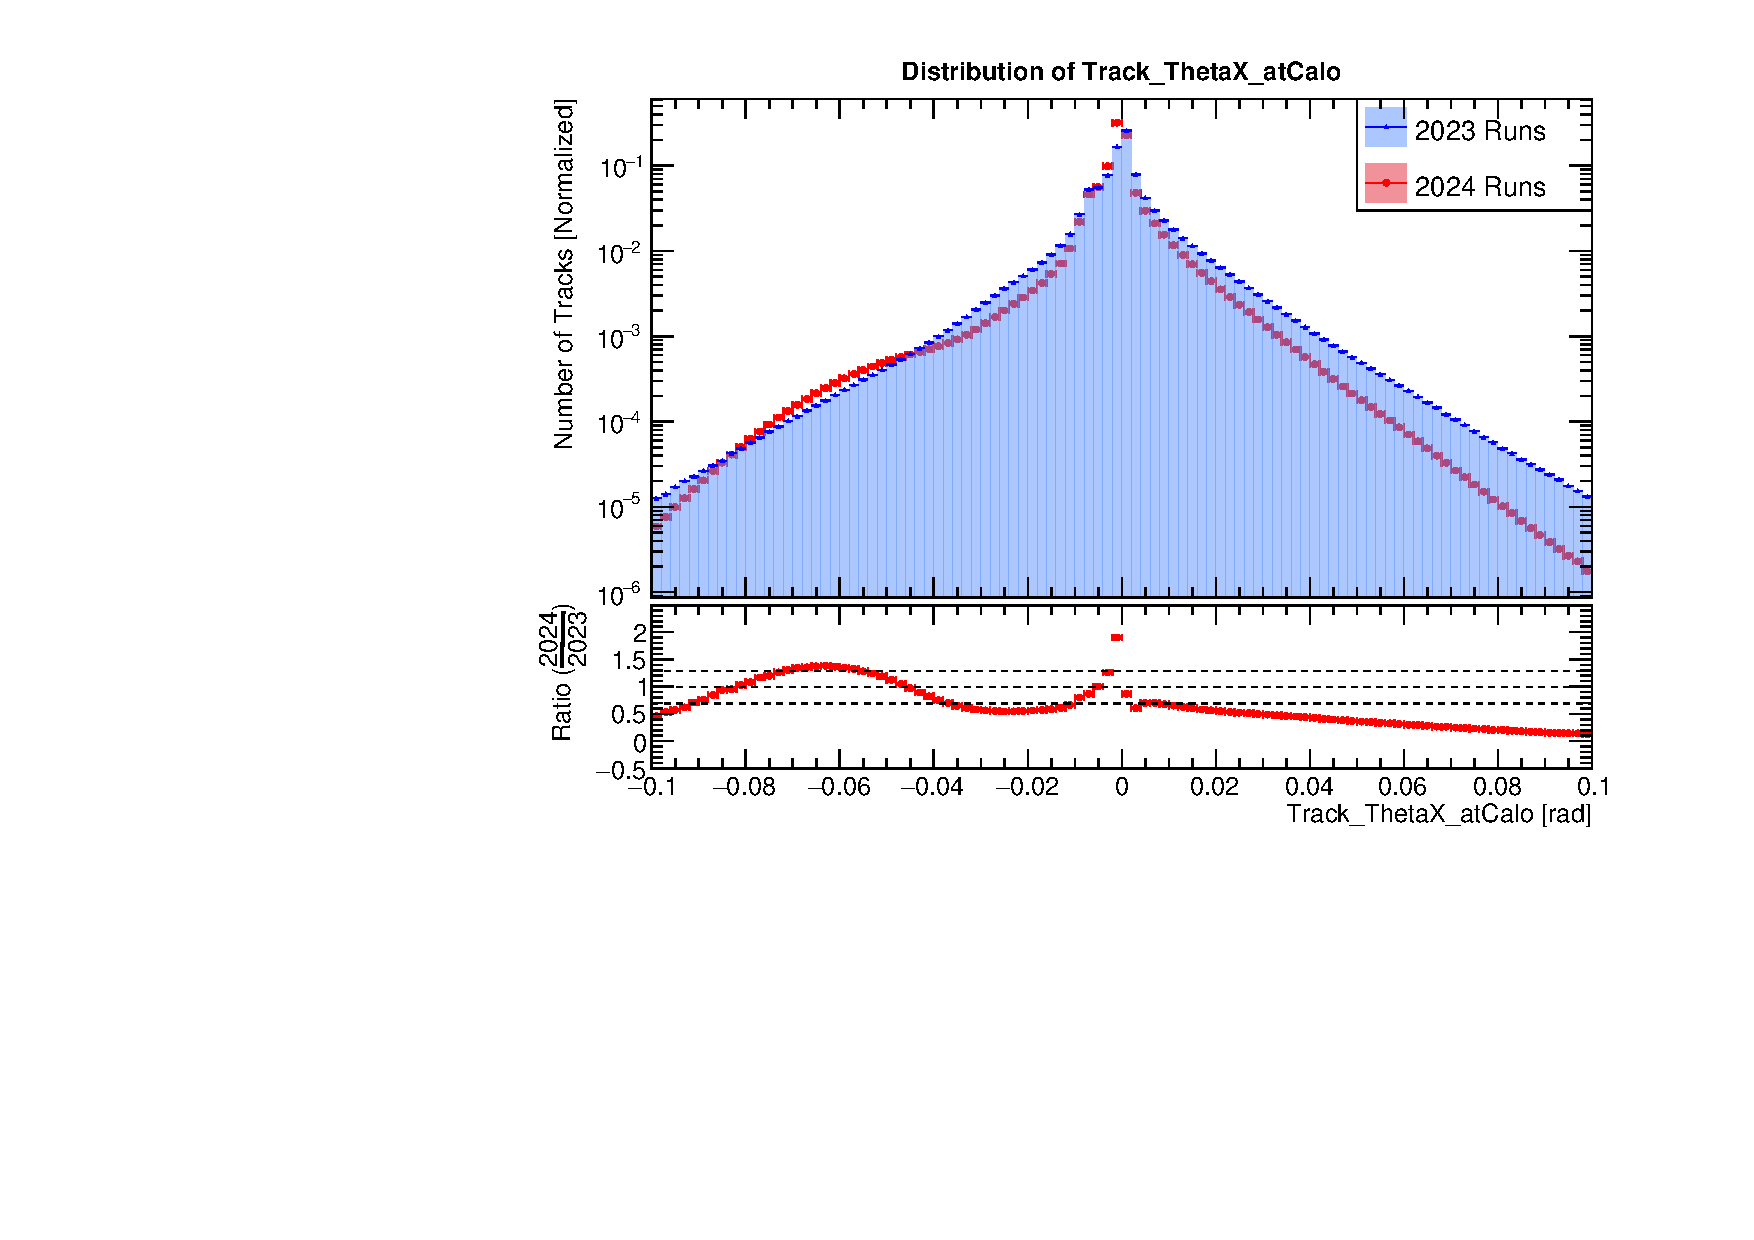
\includegraphics[width=\linewidth] {\plots/Track_ThetaX_atCalo.pdf}
				\caption{Track ThetaX at Calo}
			\end{figure}
		\end{column}
		\begin{column}{0.5\textwidth}
			\begin{figure}
				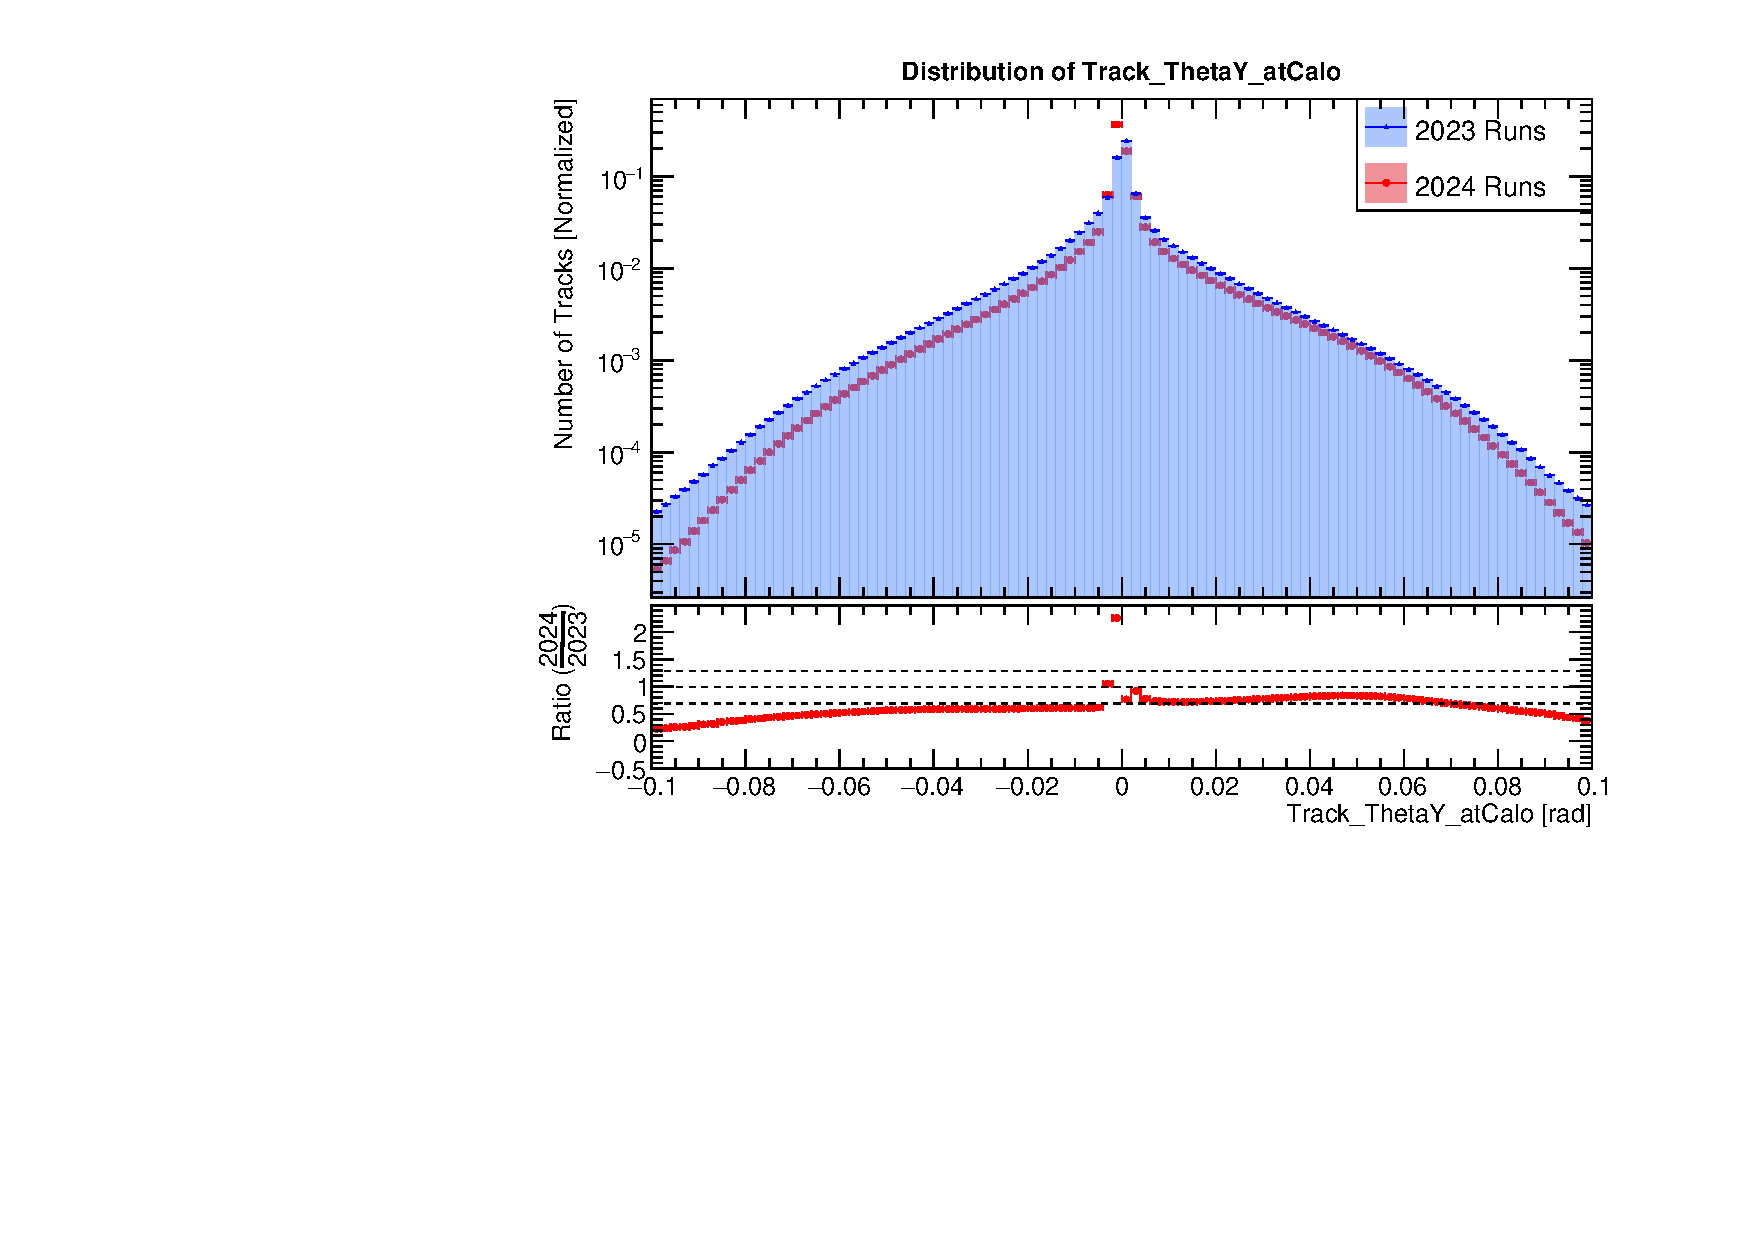
\includegraphics[width=\linewidth] {\plots/Track_ThetaY_atCalo.pdf}
				\caption{Track ThetaY at Calo}
			\end{figure}
		\end{column}
	\end{columns}
\end{frame}

\begin{frame}{Track Momenta at Tracking Station 1}
	\begin{columns}
		\begin{column}{0.5\textwidth}
			\begin{figure}
				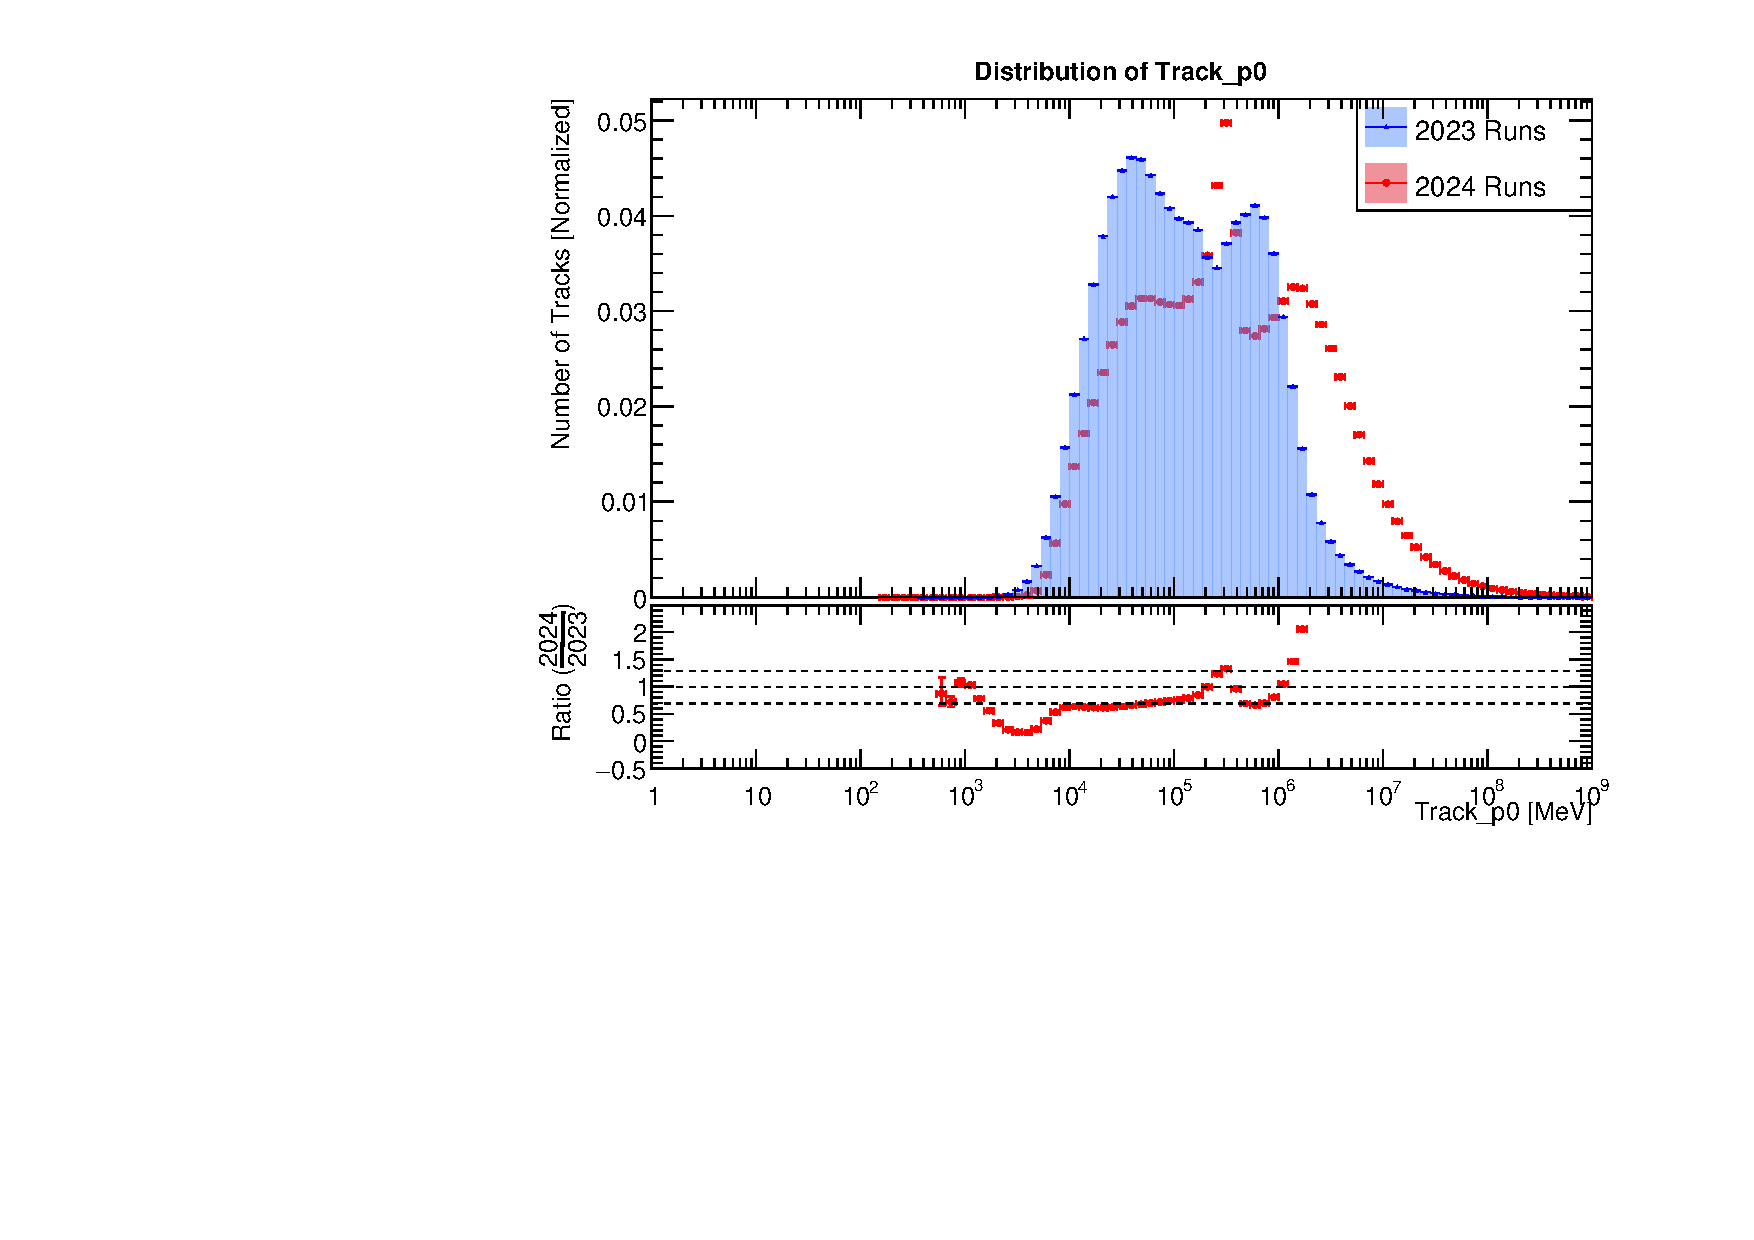
\includegraphics[width=\linewidth] {\plots/Track_p0.pdf}
				\caption{Track mometum (total) at Tracking Station 1}
			\end{figure}
		\end{column}
		\begin{column}{0.5\textwidth}
			\begin{figure}
				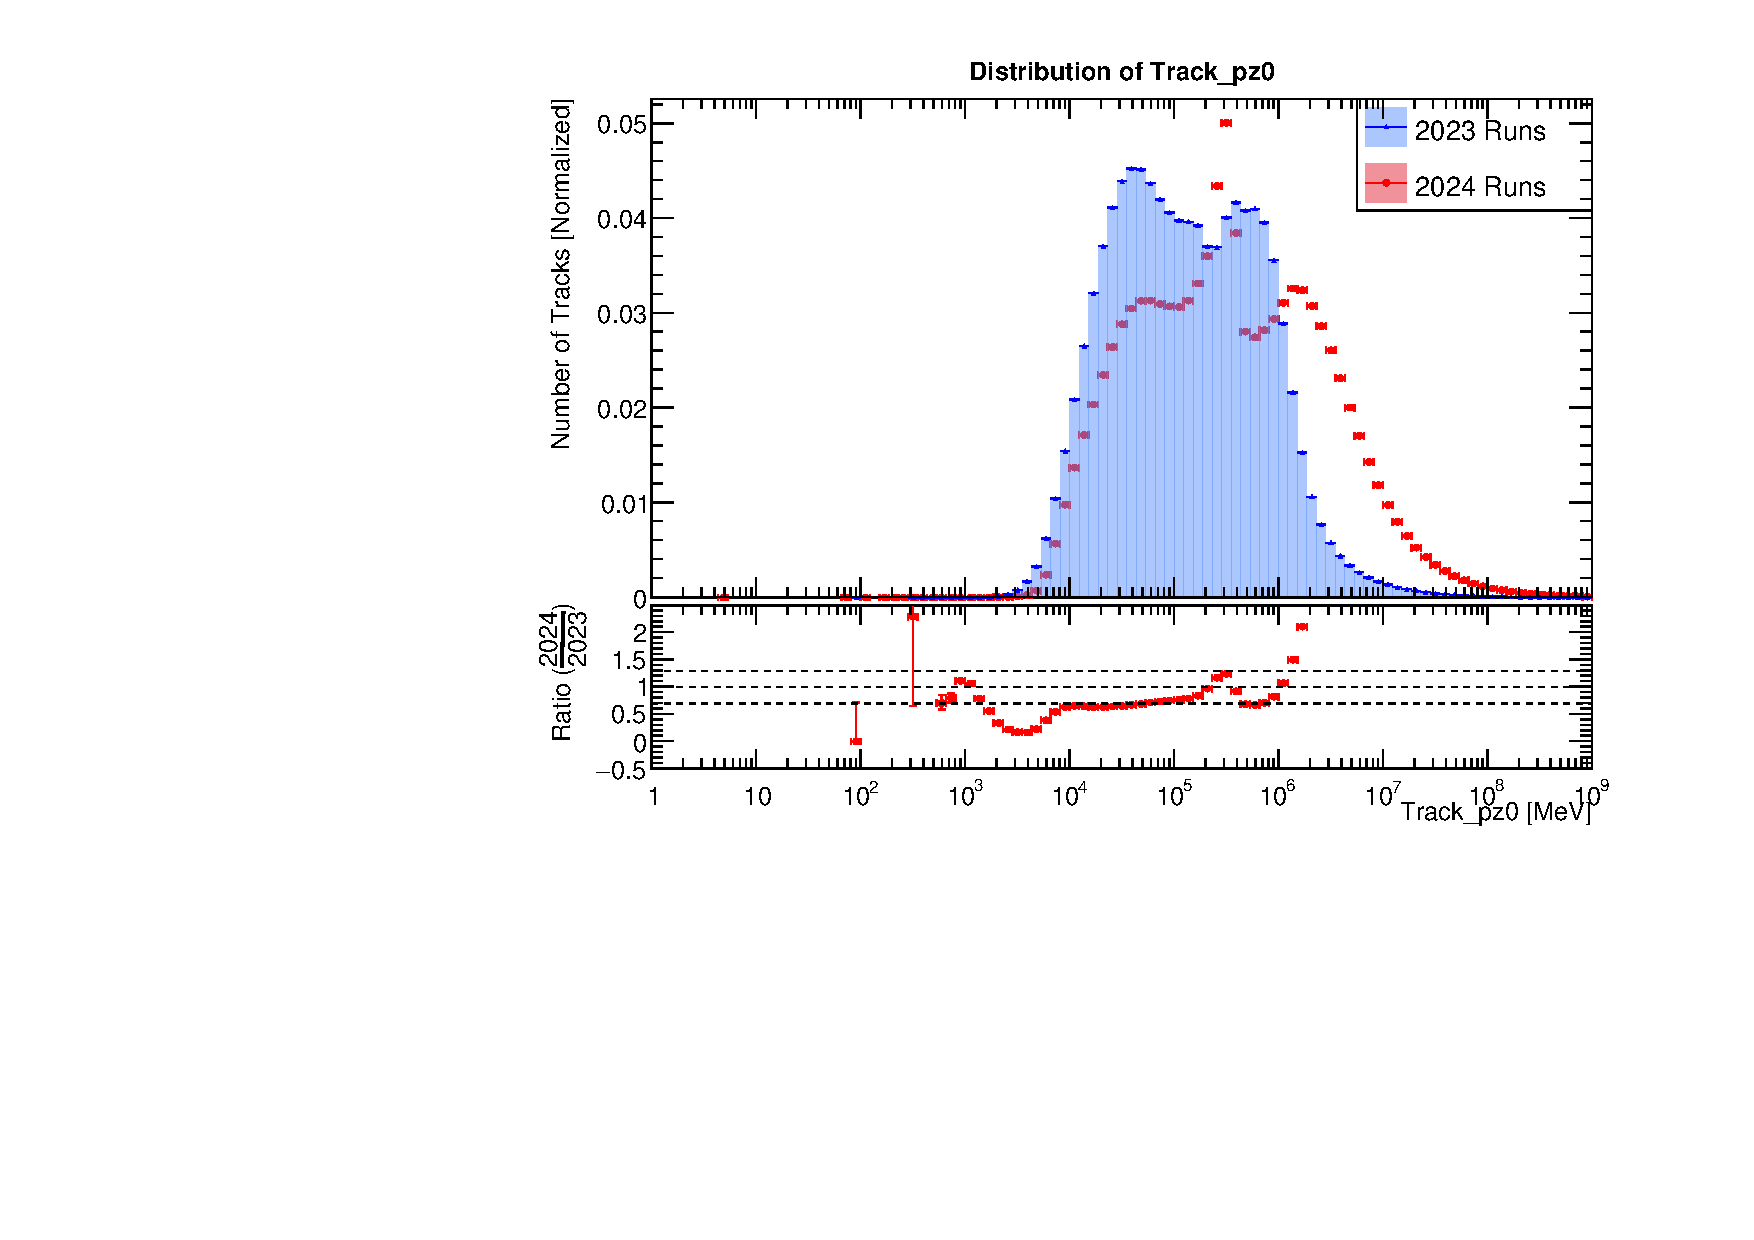
\includegraphics[width=\linewidth] {\plots/Track_pz0.pdf}
				\caption{Track momentum (pz) at Tracking Station 1}
			\end{figure}
		\end{column}
	\end{columns}
	
	\begin{itemize}
	\item We have more high momenta positively chagred muons in 2024.
	\item Background studies again showed similar features.
	\item See \href{https://indico.cern.ch/event/1350790/contributions/5686387/attachments/2836819/4957405/Introduction.pdf}{Page 15-16 of earlier talk} 
	\end{itemize}
	
\end{frame}
\begin{frame}{Runwise Plots}
    \begin{itemize}
        \item Various changes during runs
        \item NTracks/Lumi
        \item Nevent/Lumi
    \end{itemize}
\end{frame}

\begin{frame}{Runwise Plots of 2023}
    \begin{figure}
        \centering
        \includegraphics[width=1.0\textwidth]{plots_runwise/NEventsbyLumi_2023.pdf}
    \end{figure}
    \vspace{-0.35cm}
    \begin{figure}
        \centering
        \includegraphics[width=1.0\textwidth]{plots_runwise/NTracksbyLumi_2023.pdf}
    \end{figure}
\end{frame}

\begin{frame}{2024 Runs Splits}
    \begin{table}[h!]
        \begin{tabular}{|l|c|c|c|}
            \hline
            \textbf{Box}  & \textbf{Installed} & \textbf{Removed} & \textbf{Lumi (ifb)} \\ \hline
            F241          & 20/3               & 6/5              & 11.6                \\ \hline
            Tungsten only & 6/5                & 12/6             & 18.5                \\ \hline
            F242          & 12/6               & 8/7              & 9.9                 \\ \hline
            CaloNu        & 10/7               & 4/10             & 69.8                \\ \hline
            F243          & 4/10               & 22/10            & 11.9                \\ \hline
        \end{tabular}
        \caption{Table of Box Information}
    \end{table}
\end{frame}

\begin{frame}{Runwise Plots of F241- 2024}
    \begin{figure}
        \centering
        \includegraphics[width=1.0\textwidth]{plots_runwise/NEventsbyLumi_2024_F241.pdf}
    \end{figure}
    \vspace{-0.35cm}
    \begin{figure}
        \centering
        \includegraphics[width=1.0\textwidth]{plots_runwise/NTracksbyLumi_2024_F241.pdf}
    \end{figure}
\end{frame}

\begin{frame}{Runwise Plots of Tungsten only- 2024}
    \begin{figure}
        \centering
        \includegraphics[width=1.0\textwidth]{plots_runwise/NEventsbyLumi_2024_Tungsten.pdf}
    \end{figure}
    \vspace{-0.35cm}
    \begin{figure}
        \centering
        \includegraphics[width=1.0\textwidth]{plots_runwise/NTracksbyLumi_2024_Tungsten.pdf}
    \end{figure}
\end{frame}

\begin{frame}{Runwise Plots of F242- 2024}
    \begin{figure}
        \centering
        \includegraphics[width=1.0\textwidth]{plots_runwise/NEventsbyLumi_2024_F242.pdf}
    \end{figure}
    \vspace{-0.35cm}
    \begin{figure}
        \centering
        \includegraphics[width=1.0\textwidth]{plots_runwise/NTracksbyLumi_2024_F242.pdf}
    \end{figure}
\end{frame}

\begin{frame}{Runwise Plots of CaloNu - 2024}
    \begin{figure}
        \centering
        \includegraphics[width=1.0\textwidth]{plots_runwise/NEventsbyLumi_2024_CaloNu.pdf}
    \end{figure}
    \vspace{-0.35cm}
    \begin{figure}
        \centering
        \includegraphics[width=1.0\textwidth]{plots_runwise/NTracksbyLumi_2024_CaloNu.pdf}
    \end{figure}
\end{frame}

\begin{frame}{Runwise Plots of F243- 2024}
    \begin{figure}
        \centering
        \includegraphics[width=1.0\textwidth]{plots_runwise/NEventsbyLumi_2024_F243.pdf}
    \end{figure}
    \vspace{-0.35cm}
    \begin{figure}
        \centering
        \includegraphics[width=1.0\textwidth]{plots_runwise/NTracksbyLumi_2024_F243.pdf}
    \end{figure}
\end{frame}



\section{Backup}
\appendix
\appendsubframes

\end{document}